% Preambel mit Einstellungen importieren
% Document type and used packages
\documentclass[open=right, % Kapitel darf nur auf rechten Seite beginnen
paper=A4,               % DIN-A4-Papier
a4paper,                % DIN-A4-Papier
12pt,                   % Schriftgöße
headings=small,         % Kleine Überschriften
headsepline=true,       % Trennlinie am Kopf der Seite
footsepline=false,      % Trennlinie am Fuß der Seite
bibliography=totoc,     % Literaturverzeichnis in das Inhaltsverzeichnis aufnehmen
twoside=on,             % Doppelseitiger Druck - auf off stellen für einseitig
DIV=7,
cleardoublepage=plain]{scrbook} 

% Pakete einbinden, die benötigt werden
\usepackage[utf8]{inputenc}       % Dateien in UTF-8 benutzen
\usepackage[T1]{fontenc}          % Zeichenkodierung
\usepackage{graphicx}             % Bilder einbinden
\usepackage[ngerman,english]{babel}       % Deutsch und Englisch unterstützen
\usepackage{multirow}
\usepackage[table,xcdraw]{xcolor}
\usepackage{amsmath}              % Matheamtische Formeln
\usepackage{amsfonts}             % Mathematische Zeichensätze
\usepackage{amssymb}              % Mathematische Symbole
\usepackage{float}                % Fließende Objekte (Tabellen, Grafiken etc.)
\usepackage{booktabs}             % Korrekter Tabellensatz
\usepackage[printonlyused]{acronym}   % Abkürzungsverzeichnis [nur verwendete Abkürzugen]
\usepackage{makeidx}              % Sachregister
\usepackage{fancyhdr}             % Schönere Überschriften
\usepackage{listings}             % Source Code listings
\usepackage{listingsutf8}         % Listings in UTF8
\usepackage[hang,font={sf,footnotesize},labelfont={footnotesize,bf}]{caption} % Beschriftungen
\usepackage[scaled]{helvet}       % Schrift Helvetia laden
\usepackage[sf,bf,small]{titlesec} % Einstellungen für Überschriften
\usepackage[absolute]{textpos}	% Absolute Textpositionen (für Deckblatt)
\usepackage{calc}                 % Berechnung von Positionen
\usepackage{blindtext}            % Blindtexte
\usepackage[bottom=40mm,left=35mm,right=35mm,top=30mm]{geometry} % Ränder ändern
\usepackage[numbers]{natbib}       % Literaturverzeichnis nach DIN mit eckigen Klammern bei \citep
\usepackage{setspace}             % Abstände korrigieren
\usepackage{ifthen}               % Logische Bedingungen mit ifthenelse
\usepackage{scrhack}              % Get rid of tocbasic warnings
\usepackage[pagebackref=false]{hyperref}  % Hyperlinks
\usepackage[all]{hypcap}          % Korrekte Verlinkung von Floats
\usepackage{import}
\usepackage{color}
\usepackage{diagbox}
\usepackage{amssymb}

\renewcommand{\arraystretch}{1.5}

% Farben definieren
\definecolor{linkblue}{RGB}{0, 0, 100}
\definecolor{linkblack}{RGB}{0, 0, 0}
\definecolor{comment}{RGB}{63, 127, 95}
\definecolor{darkgreen}{RGB}{14, 144, 102}
\definecolor{darkblue}{RGB}{0,0,168}
\definecolor{darkred}{RGB}{128,0,0}
\definecolor{javadoccomment}{RGB}{0,0,240}

% Einstellungen für das Hyperlink-Paket
\hypersetup{
    colorlinks=true,      % Farbige links verwenden       
%    allcolors=linkblue,
    linktoc=all,          % Links im Inhaltsverzeichnis
    linkcolor=linkblack,  % Querverweise
    citecolor=linkblack,  % Literaturangaben
	filecolor=linkblack,  % Dateilinks
	urlcolor	=linkblack    % URLs
}

% Einstellungen für Quelltexte
\lstset{     
      xleftmargin=0.2cm,     
      basicstyle=\footnotesize\ttfamily,
      keywordstyle=\color{darkgreen},
      identifierstyle=\color{darkblue},
      commentstyle=\color{comment}, 
      stringstyle=\color{darkred}, 
      tabsize=2,
      lineskip={2pt},
      columns=flexible,
      inputencoding=utf8,
      captionpos=b,
      breakautoindent=true,
	  breakindent=2em,
	  breaklines=true,
	  prebreak=,
	  postbreak=,
      numbers=none,
      numberstyle=\tiny,
      showspaces=false,      % Keine Leerzeichensymbole
      showtabs=false,        % Keine Tabsymbole
      showstringspaces=false,% Leerzeichen in Strings
      morecomment=[s][\color{javadoccomment}]{/**}{*/},
      literate={Ö}{{\"O}}1 {Ä}{{\"A}}1 {Ü}{{\"U}}1 {ß}{{\ss}}2 {ü}{{\"u}}1 {ä}{{\"a}}1 {ö}{{\"o}}1
}

\urlstyle{same}

% Einstellungen für Überschriften
\titlespacing{\paragraph}{0pt}{1ex}{2.0ex}
\titlespacing{\subsubsection}{0pt}{3ex}{0.0ex}
\titlespacing{\subsection}{0pt}{4ex}{0.2ex}
\titlespacing{\section}{0pt}{7ex}{1ex}
\titleformat*{\subsubsection}{\sffamily\itshape\bfseries\small}
\titleformat*{\paragraph}{\sffamily\bfseries\small}

% Einstellungen für Schriftarten
\setkomafont{pagehead}{\normalfont\sffamily}
\setkomafont{pagenumber}{\normalfont\sffamily}
\addtokomafont{footnote}{\footnotesize}

% Wichtige Abstände
\setlength{\parskip}{0.2cm}  % 2mm Abstand zwischen zwei Absätzen
\setlength{\parindent}{0mm}  % Absätze nicht einziehen
\clubpenalty = 10000         % Keine "Schusterjungen"
\widowpenalty = 10000        % Keine "Hurenkinder"
\displaywidowpenalty = 10000 % Keine "Hurenkinder"
\renewcommand{\footnotesize}{\fontsize{9}{10}\selectfont} % Größe der Fußnoten
\setlength{\footnotesep}{8pt} % Abstand zwischen den Fußnoten

% Index erzeugen
\makeindex

% Einfacher Font-Wechsel über dieses Makro
\newcommand{\changefont}[3]{
\fontfamily{#1} \fontseries{#2} \fontshape{#3} \selectfont}

% Eigenes Makro für Bilder
\newcommand{\bild}[3]{
\begin{figure}[h]
  \centering
  \includegraphics[width=#2]{#1}
  \caption{#3}
  \label{#1}
\end{figure}}

% Wo liegt Sourcecode?
\newcommand{\srcloc}{src/}

% Wo sind die Bilder?
\graphicspath{{bilder/}}

% Makros für typographisch korrekte Abkürzungen
\newcommand{\zb}[0]{z.\,B.\ }
\newcommand{\dahe}[0]{d.\,h.\ }
\newcommand{\ua}[0]{u.\,a.\ }

\definecolor{type}{HTML}{B627A1}
\definecolor{parameter}{HTML}{7039A6}
\definecolor{class}{HTML}{302EFE}

% Dokumenteninfos importieren
% -------------------------------------------------------
% Daten für die Arbeit
% Wenn hier alles korrekt eingetragen wurde, wird das Titelblatt
% automatisch generiert. D.h. die Datei titelblatt.tex muss nicht mehr
% angepasst werden.

\newcommand{\hsmasprache}{de} % de oder en für Deutsch oder Englisch

% Titel der Arbeit auf Deutsch
\newcommand{\hsmatitelde}{Implementierung einer gestenbasierten Interaktion zum Datenaustausch zwischen mobilen Endgeräten}

% Titel der Arbeit auf Englisch
\newcommand{\hsmatitelen}{Implementation of a Gesture Based Interaction to Transfer Data Between Mobile Devices}

% Weitere Informationen zur Arbeit
\newcommand{\hsmaort}{Mannheim}    % Ort
\newcommand{\hsmaautorvname}{Benjamin} % Vorname(n)
\newcommand{\hsmaautornname}{Grab} % Nachname(n)
\newcommand{\hsmadatum}{04.03.2015} % Datum der Abgabe
\newcommand{\hsmajahr}{2015} % Jahr der Abgabe
\newcommand{\hsmafirma}{Paukenschlag GmbH, Mannheim} % Firma bei der die Arbeit durchgeführt wurde
\newcommand{\hsmabetreuer}{Prof. Kirstin Kohler, Hochschule Mannheim} % Betreuer an der Hochschule
\newcommand{\hsmazweitkorrektor}{Horst Schneider, B. Sc, Hochschule Mannheim} % Betreuer im Unternehmen oder Zweitkorrektor
\newcommand{\hsmafakultaet}{I} % I für Informatik
\newcommand{\hsmastudiengang}{IB} % IB IMB UIB IM MTB
  
% -------------------------------------------------------
% Abstract

% Kurze (maximal halbseitige) Beschreibung, worum es in der Arbeit geht auf Deutsch
\newcommand{\hsmaabstractde}{Anwender benutzen eine Vielzahl von mobilen Geräten, wie Smartphones und Tablets, um ihren täglichen Aktivitäten nachzugehen. Dabei wechseln Sie täglich mehrmals zwischen ihren Geräten, abhängig von Tätigkeit und Kontext. Bei diesem Wechsel wird jedoch der Fortschritt, der durchgeführten Tätigkeit, vom Ursprungsgerät nicht auf das Folgegerät übertragen. Der Anwender muss manuelle Maßnahmen zum Datentransfer zwischen seinen Endgeräten durchführen, die ihn von seiner eigentlichen Tätigkeit abhalten. Gestensteuerung bietet großes Potenzial, eine einfache Interaktion für den Anwender zu bieten, mit der Daten übertragen werden können. Diese Arbeit untersucht deshalb die gestenbasierte Bump-Interaktion, bei der durch einfaches Anstoßen eines Endgeräts Daten auf ein anderes zur Synchronisierung übertragen werden. Im Rahmen dieser Arbeit wird diese Geste analysiert, verschiedene Konzepte für eine Umsetzung erarbeitet, Vor- und Nachteile der Entwürfe dargestellt und einer der Entwürfe prototypisch umgesetzt.}

% Kurze (maximal halbseitige) Beschreibung, worum es in der Arbeit geht auf Englisch

\newcommand{\hsmaabstracten}{On a daily basis people use several mobile devices, like Smartphones or Tablets, to fullfil all kinds of tasks. While doing so they often switch from one devices to another to leverage all the advantages of their device like screen size. When the user switches his device while performing some task he has to manually transfer data to the new device, to continue the task, he has begun on the previous device. For the user this manual data transfer is tedious and keeps him from doing, what he actually wants to do. He just wants to continue, where he left off, when he switches devices. Gesture based interactions can be used, to solve this problem. With the bump-gesture there is already a known interaction which can be used to transfer data between devices. This thesis dicusses design and development of the bump gesture. It analyses the bump-gesture, shows several system designs, discusses advantages and disadvantages of the desings and implements a prototype Application based on one of the designs.
 }





\begin{document}
\frontmatter

% Römische Ziffern für die "Front-Matter"
\setcounter{page}{0}
\changefont{ptm}{m}{n}  % Times New Roman für den Fließtext
\renewcommand{\rmdefault}{ptm}

% Titelblatt
% -------------------------------------------------------
% In dieser Datei sollten eigentlich keine Veränderungen mehr
% notwendig sein.
% -------------------------------------------------------

\thispagestyle{empty}

\ifthenelse{\equal{\hsmafakultaet}{I}}%
  {\newcommand{\hsmafakultaetlangde}{Fakultät für Informatik}%
   \newcommand{\hsmafakultaetlangen}{Department of Computer Science}}{}

\ifthenelse{\equal{\hsmastudiengang}{IB}}%
  {\newcommand{\hsmastudienganglangde}{Informatik}%
  \newcommand{\hsmastudienganglangen}{Computer Science}%
  \newcommand{\hsmatypde}{Bachelor-Thesis}%
  \newcommand{\hsmatypen}{Bachelor Thesis}%
  \newcommand{\hsmagrad}{\hsmabsc}}{}

\ifthenelse{\equal{\hsmastudiengang}{IMB}}%
  {\newcommand{\hsmastudienganglangde}{Medizinische Informatik}%
  \newcommand{\hsmastudienganglangen}{Medical Informatics}%
  \newcommand{\hsmatypde}{Bachelor-Thesis}%
  \newcommand{\hsmatypen}{Bachelor Thesis}%
  \newcommand{\hsmagrad}{\hsmabsc}}{}
  
\ifthenelse{\equal{\hsmastudiengang}{UIB}}%
  {\newcommand{\hsmastudienganglangde}{Unternehmens- und Wirtschaftsinformatik}%
  \newcommand{\hsmastudienganglangen}{Enterprise Computing}%  
  \newcommand{\hsmatypde}{Bachelor-Thesis}%
  \newcommand{\hsmatypen}{Bachelor Thesis}%
  \newcommand{\hsmagrad}{\hsmabsc}}{}

\ifthenelse{\equal{\hsmastudiengang}{IM}}%
  {\newcommand{\hsmastudienganglangde}{Informatik}%
   \newcommand{\hsmastudienganglangen}{Computer Science}%
   \newcommand{\hsmatypde}{Master-Thesis}%
   \newcommand{\hsmatypen}{Master Thesis}%
   \newcommand{\hsmagrad}{\hsmamaster}}{}

\ifthenelse{\equal{\hsmastudiengang}{MTB}}%
  {\newcommand{\hsmastudienganglangde}{Mechatronik}%
   \newcommand{\hsmastudienganglangen}{Mechatronics}%
   \newcommand{\hsmatypde}{Bachelor-Thesis}%
   \newcommand{\hsmatypen}{Bachelor Thesis}%
   \newcommand{\hsmagrad}{\hsmabsc}}{}

\newcommand{\hsmabsc}{Bachelor of Science (B.Sc.)}
\newcommand{\hsmamaster}{Master of Science (M.Sc.)}

\newcommand{\hsmakoerperschaftde}{Hochschule Mannheim}
\newcommand{\hsmakoerperschaften}{University of Applied Sciences Mannheim}

\newcommand{\hsmaautorbib}{\hsmaautornname, \hsmaautorvname} % Autor Nachname, Vorname
\newcommand{\hsmaautor}{\hsmaautorvname \ \hsmaautornname} % Autor Vorname Nachname

\ifthenelse{\equal{\hsmasprache}{de}}%
  {\newcommand{\hsmatyp}{\hsmatypde}%
   \newcommand{\hsmathesistype}{zur Erlangung des akademischen Grades \hsmagrad}%
   \newcommand{\hsmakoerperschaft}{\hsmakoerperschaftde}%
   \newcommand{\hsmastudiengangname}{Studiengang \hsmastudienganglangde}%
   \newcommand{\hsmastudienganglang}{\hsmastudienganglangde}%
   \newcommand{\hsmatitel}{\hsmatitelde}%
   \newcommand{\hsmatutor}{Betreuer}%
   \newcommand{\hsmafakultaetlang}{\hsmafakultaetlangde}%
   \selectlanguage{ngerman}}%
  {\newcommand{\hsmatyp}{\hsmatypen}%
   \newcommand{\hsmathesistype}{for the acquisition of the academic degree \hsmagrad}%
   \newcommand{\hsmakoerperschaft}{\hsmakoerperschaften}%
   \newcommand{\hsmastudiengangname}{Course of Studies: \hsmastudienganglang}%
   \newcommand{\hsmastudienganglang}{\hsmastudienganglangen}%
   \newcommand{\hsmatitel}{\hsmatitelen}%
   \newcommand{\hsmatutor}{Tutors}
   \newcommand{\hsmafakultaetlang}{\hsmafakultaetlangen}%
   \selectlanguage{english}}%


% Daten in die Standard Felder von KOMA-Script eintragen
\titlehead{\hsmatyp im \  \hsmastudienganglang}
\subject{}
\title{\hsmatitel}
\author{\hsmaauthor}
\date{\small{\hsmadatum}}

% Daten für das fertige PDF-Dokument
\hypersetup{
  pdftitle={\hsmatitel},  % Titel des Dokuments
  pdfauthor={\hsmaautor},              % Autor
  pdfsubject={\hsmatyp im \ \hsmastudienganglang},                % Thema
  pdfkeywords={\hsmatitel}         % Schlüsselworte
}

\newlength{\bindekorrektur}
\newlength{\seitenanfang}
\newlength{\seitenbreite}
  
\setlength{\bindekorrektur}{-46mm}   % Korrektur der horizontalen Position
\setlength{\seitenanfang}{0mm}       % Korrektur der vertikalen Position
\setlength{\seitenbreite}{297mm}

\noindent
\includegraphics[width=7cm]{hsma-logo.pdf}\\

% Titel der Arbeit
\begin{textblock*}{128mm}(45mm,\seitenanfang + 62mm) % 4,5cm vom linken Rand und 6,0cm vom oberen Rand
  \centering\Large\sffamily
  \vspace{4mm} % Kleiner zusätzlicher Abstand oben für bessere Optik
  \textbf{\hsmatitel}
\end{textblock*}%

% Name
\begin{textblock*}{128mm}(45mm,\seitenanfang + 103mm)
  \centering\large\sffamily
  \hsmaautor
\end{textblock*}

% Thesis
\begin{textblock*}{\seitenbreite}(\bindekorrektur,\seitenanfang + 130mm)
  \centering\large\sffamily
  \hsmatyp\\
  \begin{small}\hsmathesistype \end{small}\\
  \vspace{2mm}
  \hsmastudiengangname
\end{textblock*}

% Fakultät
\begin{textblock*}{\seitenbreite}(\bindekorrektur,\seitenanfang + 165mm)
  \centering\large\sffamily
  \hsmafakultaetlang\\
  \vspace{2mm}
  \hsmakoerperschaft
\end{textblock*}

% Datum
\begin{textblock*}{\seitenbreite}(\bindekorrektur,\seitenanfang + 190mm)
  \centering\large 
  \textsf{\hsmadatum}
\end{textblock*}

% Firma
\begin{textblock*}{\seitenbreite}(\bindekorrektur,\seitenanfang + 215mm)
  \centering\large 
  %\textsf{Durchgeführt bei der Firma \hsmafirma}
\end{textblock*}

% Betreuer
\begin{textblock*}{\seitenbreite}(\bindekorrektur,\seitenanfang + 240mm)
  \centering\large\sffamily
  \hsmatutor \\
  \vspace{2mm}
  \hsmabetreuer\\
  \vspace{2mm}
  \hsmazweitkorrektor
\end{textblock*}

% Bibliographische Informationen
\null\newpage
\thispagestyle{empty}
  
\newcommand{\hsmabibde}{\begin{small}\textbf{\hsmaautorbib}: \\ \hsmatitelde \ / \hsmaautor. \ -- \\ \hsmatyp, \hsmaort \ : \hsmakoerperschaftde, \hsmajahr. \pageref{lastpage} Seiten.\end{small}}

\newcommand{\hsmabiben}{\begin{small}\textbf{\hsmaautorbib}: \\ \hsmatitelen \ / \hsmaautor. \ -- \\ \hsmatyp, \hsmaort \ : \hsmakoerperschaften, \hsmajahr. \pageref{lastpage} pages. \end{small}}

\ifthenelse{\equal{\hsmasprache}{de}}%
  {\hsmabibde \\ \vspace{0.5cm} \\ \hsmabiben}
  {\hsmabiben \\ \vspace{0.5cm} \\ \hsmabibde}


% Erklärung
\clearpage\setcounter{page}{1}
\thispagestyle{empty}
\textsf{\large\textbf{Erklärung}}

Hiermit erkläre ich, dass ich die vorliegende Arbeit selbstständig verfasst und keine anderen als die angegebenen Quellen und Hilfsmittel benutzt habe.

\vspace{1cm}
\hsmaort, \hsmadatum \\

\vspace{1.2cm}						                                      
\hsmaautor
\cleardoublepage

% Abstract
\chapter*{Abstract}

\ifthenelse{\equal{\hsmasprache}{de}}%
  {\subsubsection*{\hsmatitelde}\hsmaabstractde\subsubsection*{\hsmatitelen}\hsmaabstracten}
  {\subsubsection*{\hsmatitelen}\hsmaabstracten\subsubsection*{\hsmatitelde}\hsmaabstractde}


% Inhaltsverzeichnis erzeugen
\tableofcontents

% Korrigiert Nummerierung bei mehrseitigem Inhaltsverzeichnis
\cleardoublepage
\newcounter{frontmatterpage}
\setcounter{frontmatterpage}{\value{page}}

% Arabische Zahlen für den Hauptteil
\mainmatter

% Den Hauptteil mit vergrößertem Zeilenabstand setzen
\onehalfspacing

% ------------------------------------------------------------------
% Hauptteil der Arbeit
 \chapter{Einleitung}
\label{Kap1}
\label{chap:Kap1}

\section{Problemstellung}
Immer mehr Anwender nutzen nicht mehr exklusiv den Desktop PC, sondern eine Vielzahl an Endgeräten um ihren täglichen Aktivitäten nachzugehen. Abhängig vom Kontext, das heißt von Ziel, Aufenthaltsort und Zeitpunkt, entscheiden Anwender, welche Geräte sich für eine Situation am besten eignen und treffen entsprechend eine Auswahl \cite{Google2014:Online}. Dabei kann es vorkommen, dass zur Erledigung einer Aufgabe, mehrere Geräte gleichzeitig oder aufeinanderfolgend genutzt werden. Dadurch lassen sich die Vorteile der verschiedenen Geräte, wie Bildschirmgröße, Mobilität oder Interaktionsmöglichkeiten ausnutzen. Nach einer Studie von Google ist dieses multi-screening bei einem Großteil der Anwender zu beobachten. So beginnen beispielsweise 90\% der in der Studie befragten Personen eine Aktivität auf einem Gerät und führen diese zu einem späteren Zeitpunkt auf einem anderen Gerät fort \cite{Google2014:Online}. Für den Anwender ist diese vermischte Nutzung von Endgeräten somit ein alltäglicher Vorgang. Damit ein Anwender seine Aktivität bei einem Gerätewechsel fortsetzen kann, müssen häufig erst Daten zwischen den Geräten ausgetauscht werden. Dieser Datenaustausch geschieht häufig nicht automatisch und erfordern vom Anwender eine Reihe von komplizierten Interaktionen zum Datentransfer zwischen den Geräten. Für den Anwender stellt dies eine Störung seines Arbeitsablaufes dar. Er erwartet fließend zwischen Geräten wechseln zu können da er seine Aktivität über Gerätegrenzen hinaus als zusammengehörig empfindet.

Mit Gestensteuerung können Interaktionen verwirklicht werden, die über Gerätegrenzen hinaus wirken. Somit kann der für den Anwender aufwendige  Interaktionen zur Datenübertragung beim Gerätewechsel durch eine einzelne intuitive Interaktion durchgeführt werden. Ein vielversprechender Kandidat für solch eine Interaktion ist die Bump-Geste. Die Bump-Geste ist eine Interaktion, bei der Daten zwischen Endgeräten ausgetauscht werden indem diese sich gegenseitig anstoßen (bumpen). Anwender, die ihr Gerät wechseln, wollen mit dem Gerät, auf dem die Aktivität begonnen wurde, das Folgegerät bumpen und damit alle notwendigen Daten übertragen, um ihre Aktivität sofort auf dem neuen Gerät weiterzuführen zu können. Betrachtet ein Anwender z.B. ein Photoalbum auf seinem Smartphone und möchte diese Aktivität auf seinem Tablet fortsetzen, muss er nur das Smartphone an das Tablet bumpen. Anschließend wird das Photoalbum auf das Tablet übertragen und die Applikation navigiert automatisch zu Photoalbum und Bild, bei dem die Aktivität auf dem Smartphone beendet wurde.

\section{Ziel der Arbeit}
Das Ziel dieser Arbeit ist es, verschiedene Systementwürfe zu identifizieren und zu beschreiben, mit denen die Bump Interaktion realisiert werden kann. Diese Entwürfe berücksichtigen unterschiedliche technische Rahmenbedingungen und werden auf ihre Vor- und Nachteile geprüft. und Aufbauend auf einem der identifizierten Systementwürfe wird eine Demonstrator Applikation entwickelt mit der ein aktives Dokument oder Foto auf ein anderes Gerät übertragen werden kann.

\section{Aufbau der Arbeit}
In Kapitel \ref{chap:Kap2} werden verwandte Arbeiten und Applikationen zum Thema sowie Technische Grundlagen beschrieben. Kapitel \ref{chap:Kap3} analysiert und beschreibt die Bump-Interaktion. Kapitel \ref{chap:Kap4} beschreibt einleitend Grundlagen zu relevanten iOS Frameworks auf deren Basis  Konzepte zur Bump Erkennung, Geräte Identifizierung und zum Datenaustausch beschrieben und verglichen werden. In Kapitel \ref{chap:Kap5} wird die entwickelte Demonstrator Applikation vorgestellt. Abschließend bietet Kapitel \ref{chap:Kap6} eine Zusammenfassung über die erarbeiteten Ergebnisse und einen Ausblick auf zukünftige potenzielle Weiterentwicklungen der Arbeit. Die Bedeutungen der verwendeten Abkürzungen befinden sich im \nameref{Abk} und ein Überblick der dargestellten Abbildungen im Abbildungsverzeichnis sowie der Tabellen im Tabellenverzeichnis. Zudem ist die verwendete Literatur im Literaturverzeichnis angegeben. % Externe Datei einbinden
\chapter{Stand der Technik}
\label{Kap2}
\label{chap:Kap2}

Im folgenden Kapitel werden verwandte Arbeiten und Applikationen zum Thema sowie Technisches Grundlagenwissen, das zur Umsetzung der Interaktion benötigt wird, beschrieben.

\section{Grundlagen zum gestenbasierten Transfer von Daten}

Die Nutzung einer gestenbasierten Interaktion zum Datenaustausch wurde schon von einigen wissenschaftlichen Arbeiten behandelt und in Applikationen umgesetzt. An dieser Stelle wird eine Auswahl an Arbeiten und Applikationen vorgestellt die Ähnlichkeit mit der geplanten Bump-Interaktion aufweisen.

\textbf{Hinckley} \cite{Hinckley:2003:SGM:964696.964713} beschreibt eine Interaktion, mit der Tablet-Computer über eine Bump-Interaktion miteinander verbunden werden. Das anstoßen der Geräte aneinander (Siehe Abbildung \ref{fig:hinckley}) baut eine Verbindung zwischen den Geräten auf, indem die generierten Accelerometer Daten zusammen mit einem Timestamp über ein lokales WLAN-Netzwerk ausgetauscht und abgeglichen werden. Die Bump-Interaktion entwickelt Hinckley auf der Metapher des Anstoßens von zwei Trinkgläsern aneinander. Deshalb führt er die Trinkgläser-Metapher auch für den Datenaustausch fort und definiert eine Geste, die dem umschütten von Flüssigkeit aus einem Glas in ein anderes entspricht. Dieser Metapher folgend, schüttet eines der Geräte ausgewählte Daten durch eine drehende Bewegung in das andere Gerät (Siehe Abbildung \ref{fig:hinckley2}).

\begin{figure}[H]
\begin{minipage}[h]{7cm}
	\centering
	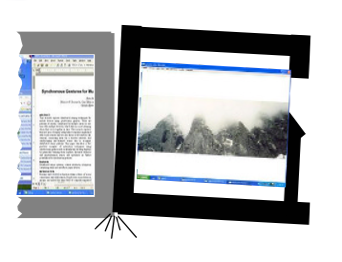
\includegraphics[width=5cm]{kapitel2/hinkley.png}
	\caption{Bump Tablet-Computer \cite{Hinckley:2003:SGM:964696.964713}}
	\label{fig:hinckley}
\end{minipage}
\hfill
\begin{minipage}[h]{7cm}
	\centering
	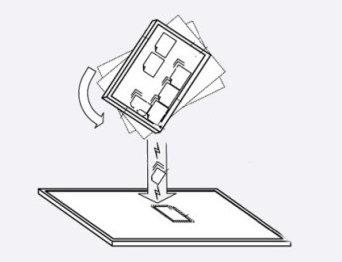
\includegraphics[width=5cm]{kapitel2/hinkley2.png}
	\caption{Daten ausschütten \cite{HinkleyPic2:Online}}
	\label{fig:hinckley2}
\end{minipage}
\end{figure}


Ähnlich wie bei Hinckley werden bei der Applikation \textbf{Bump} \cite{Bump:Online} die Beschleunigungssensoren von Smartphones und Tablets genutzt um Bump-Events festzustellen (Siehe Abbildung \ref{fig:bumpPhone}). Die Applikation sendet, nachdem ein Bump festgestellt wurde, die ausgewählten Nutzdaten, sowie Charakteristiken des Bumps an einen Server. Der Sever erkennt eingehende Bumps durch einen Algorithmus und ordnet Bump-Partner basierend auf den Charakteristiken der Bumps einander zu. Der Algorithmus nutzt unter anderem GPS-Standortdaten, um die Anzahl der möglichen Treffer zu reduzieren, sowie eine Anzahl anderer Daten, um die richtigen Bump-Partner zu identifizieren. Nachdem der Server die Geräte einander zugeordnet hat, leitet er die entsprechenden Nutzdaten an die jeweiligen Geräte weiter. Der Datenaustausch zwischen mobilen Endgeräten und Computern ist auch möglich. Dazu muss das mobile Gerät auf die Leertaste der Computertastatur gebumped werden (Siehe Abbildung \ref{fig:bumpPC}).

\begin{figure}[H]
\begin{minipage}[h]{7cm}
	\centering
	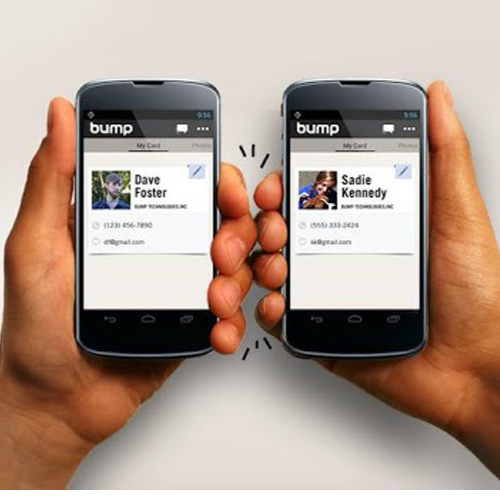
\includegraphics[width=5.5cm]{kapitel2/bumpPhone.png}
	\caption{Bump-Geste Smartphones \cite{BumpPicPhone:Online}}
	\label{fig:bumpPhone}
\end{minipage}
\hfill
\begin{minipage}[h]{7cm}
	\centering
	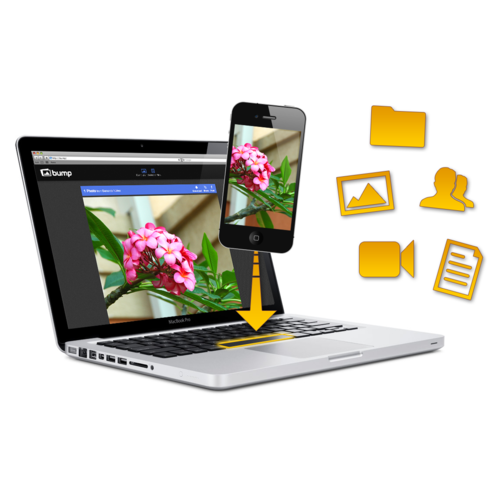
\includegraphics[width=5.5cm]{kapitel2/bumpPC.png}
	\caption{Bump-Geste PC \cite{Bump:Online}}
	\label{fig:bumpPC}
\end{minipage}
\end{figure}

\textbf{Yatani et al.} \cite{Yatani:2006:TII:1184855.1184874} nutzen Accelerometer Daten um Wurf- und Schwung-Gesten zu erkennen. Mit einer Wurf-Geste werden Daten, zu einem einzelnen Empfänger geworfen. Durch eine Schwung Geste können mehrere Geräte auf einmal als Empfänger ausgewählt werden. Der Datenaustausch erfolgt über einen Server in einem lokalen \acs{WLAN}-Netzwerk. Der Server ist ebenfalls dafür zuständig, die Position und Orientierung der Geräte zu verarbeiten, um so Sender und Empfänger einander zuzuordnen. Für die Positionsbestimmung wird ein speziell entwickeltes System genutzt, mit dem die Position und Orientierung der Endgeräte über eine Kamera erkannt wird.

\begin{figure}[H]
\begin{minipage}[h]{7cm}
	\centering
	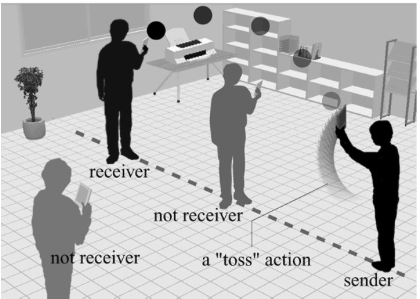
\includegraphics[width=5.5cm]{kapitel2/yatani1.png}
	\caption{Wurf- und Fang-Geste \cite{Yatani:2006:TII:1184855.1184874}}
	\label{fig:yatani1}
\end{minipage}
\hfill
\begin{minipage}[h]{7cm}
	\centering
	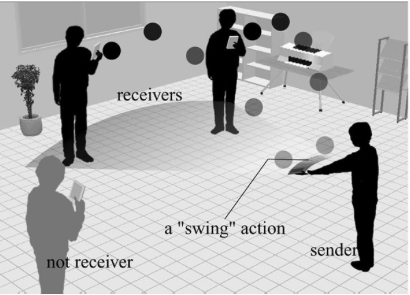
\includegraphics[width=5.5cm]{kapitel2/yatani2.png}
	\caption{Schwung-Geste \cite{Yatani:2006:TII:1184855.1184874}}
	\label{fig:yatani2}
\end{minipage}
\end{figure}

\textbf{Hoccer} ist eine Applikation, die über zwei Gesten verfügt, mit denen Daten zwischen Endgeräten ausgetauscht werden können. Zum einen gibt es die Swipe Geste (Siehe Abbildung \ref{fig:hocSwipe}) und zum anderen eine Wurf und Fang Geste, die vergleichbar mit der Geste von Yatani et al. ist. Mit der Swipe Geste wird über den Touchscreen eine geöffnete Datei von einem Gerät auf das andere geschoben. Bei der Wurf und Fang Geste, führt ein Anwender die Wurf Geste aus und wirft einem zweiten Anwender die Daten, wie mit einem Frisbee, zu. Dieser muss sich als Empfänger identifizieren indem er sein Endgerät nach oben hält, als wollte er das Frisbee fangen. Die Applikation funktioniert technisch ähnlich wie Bump über \acs{GPS}-Standortdaten mit einem Server, der Geräte zuordnet und den Datenverkehr zwischen den Geräten steuert. \cite{Hoccer:Online}

\begin{figure}[H]
	\centering
	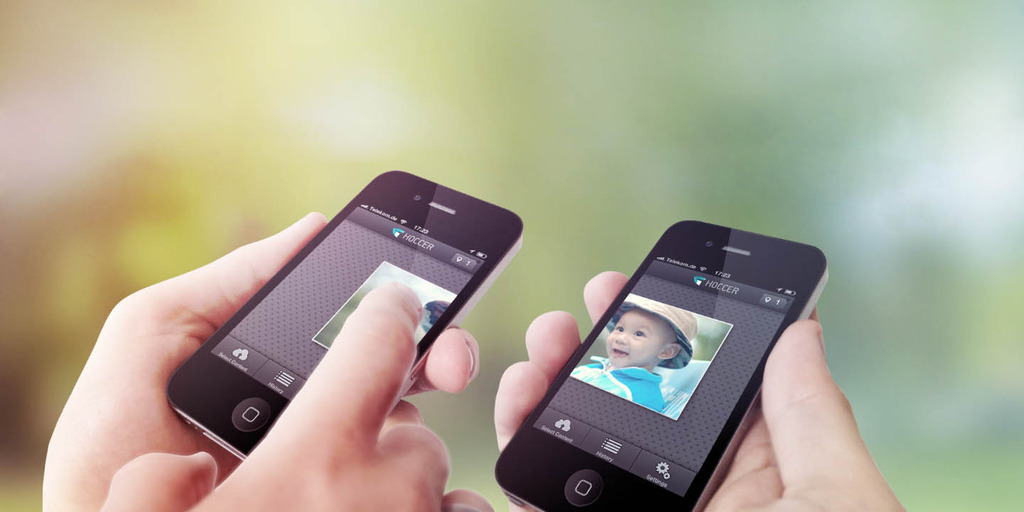
\includegraphics[width=8cm]{kapitel2/hoccerSwipe.jpg}
	\caption{Hoccer Swipe-Geste \cite{HoccerPics:Online}}
	\label{fig:hocSwipe}
\end{figure}

\paragraph{Lucero et al.} \cite{Lucero:2011:PCU:1978942.1979201} haben ein Gesten-gesteuertes System entwickelt, mit dem eine Gruppe von Personen ihre auf Smartphones gespeicherten Photosammlungen durchblättern und untereinander Photos austauschen können. Dazu müssen die Smartphones aller Anwender zusammen auf einem Tisch liegen, am besten in einem Kreis angeordnet. Mit der Hilfe von Gesten kann jeder Anwender durch seine individuelle Photosammlung blättern. Dazu muss er das Smartphone rechts kippen um ein Photo weiterzublättern (Siehe Abbildung \ref{fig:passtThem1}) oder nach links kippen um zurückzublättern. Durch einen Tap auf den Touchscreen rechts oder links kann auch entsprechend vor oder zurückgeblättert werden. Möchte ein Anwender ein einzelnes Bild teilen, muss er so lange die Tap-Geste auf dem Touchscreen ausführen bis eine Miniaturansicht des ausgewählten Photos erscheint. Dieses Bild kann anschließend durch eine Swipe-Geste in die Richtung des Zielgeräts auf dieses übertragen werden. Das System nutzt Accelerometer Daten, um die Geste zum weiterblättern zu erkennen und tauscht die Daten zwischen den Geräten über ein WLAN Netzwerk aus. Für die Identifizierung des Zielgeräts beim Datenaustausch wurde ein spezielles Multi-Emitter Tracking System verwendet, mit dem die Position der Endgeräte festgestellt werden kann.

\begin{figure}[H]
\begin{minipage}[h]{7cm}
	\centering
	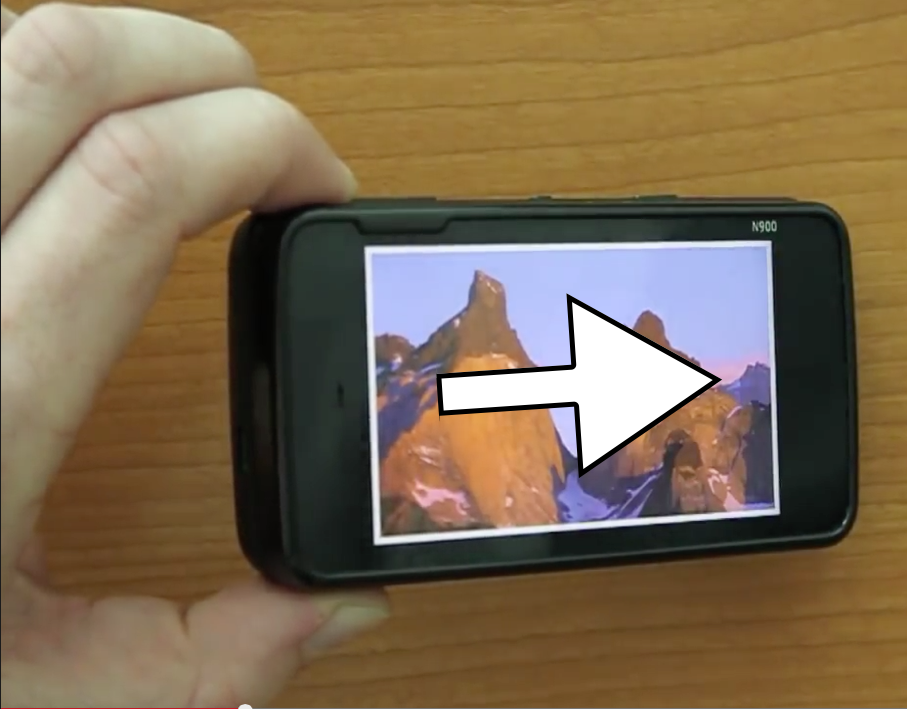
\includegraphics[width=6.5cm]{kapitel2/passThem1.png}
	\caption{Links kippen zum weiterblättern \cite{Lucero:2011:PCU:1978942.1979201}}
	\label{fig:passtThem1}
\end{minipage}
\hfill
\begin{minipage}[h]{7cm}
	\centering
	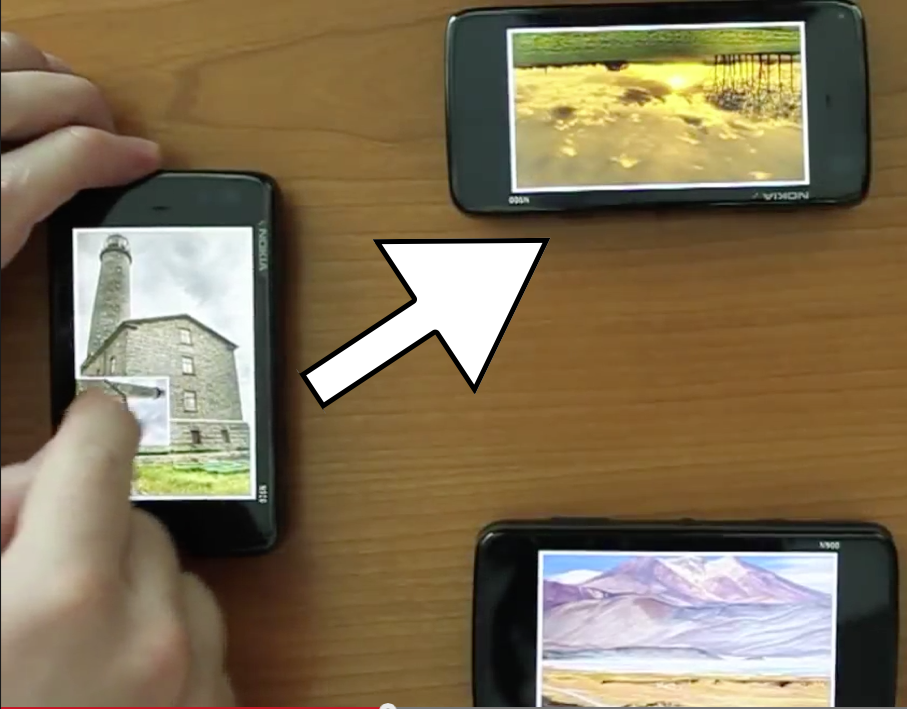
\includegraphics[width=6.5cm]{kapitel2/passThem2.png}
	\caption{Schwung-Geste Auswahl mehrerer Ziele \cite{Lucero:2011:PCU:1978942.1979201}}
	\label{fig:beamTransfer}
\end{minipage}
\end{figure}

\newpage
\section{Technische Grundlagen}
Mobile Endgeräte stecken voller Technologien, um ihre Umwelt wahrzunehmen und mit ihr zu kommunizieren. Dieser Abschnitt identifiziert Technologien zu Datenübertragung, Positionsortung und Sensorik, die für die Implementierung der Bump-Interaktion in Frage kommen.

\subsection{Technologien zur Datenübertragung}

\subsubsection{WLAN}
Ein \ac{WLAN} ist ein lokales Funknetz, das auf der Normenfamilie \acs{IEEE} 802.11 basiert und sich über eine Reichweite von 30 - 100 Meter aufspannen kann. Ein solches Netzwerk kann entweder im Infrastruktur-Modus oder im Ad-hoc-Modus betrieben werden. Der Infrastruktur-Modus ist topologisch wie ein Stern (Siehe Abbildung \ref{fig:topo}) aufgebaut. Endgeräte melden sich an einer zentralen Basisstation an und können danach über diese miteinander kommunizieren. Im Ad-hoc-Modus bauen Endgeräte eine direkte Verbindung miteinander auf ohne den Umweg über eine gesonderte Basistation. Jedes Endgerät kann mehrere Verbindungen zu anderen Geräten unterhalten, womit ein vermaschtes Netzwerk (Siehe Abbildung \ref{fig:topo}) gebildet wird \cite[46-55]{baun2012computernetze}.  

\begin{figure}[H]
\begin{minipage}[h]{7cm}
  \centering
  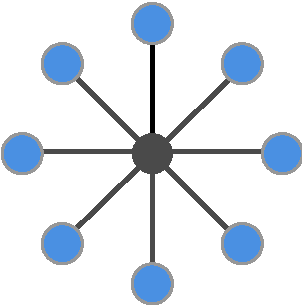
\includegraphics[width=5cm]{kapitel2/SternTopologie.pdf}
  Stern-Topologie
\end{minipage}
\hfill
\begin{minipage}[h]{7cm}
  \centering
  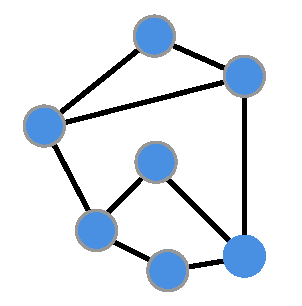
\includegraphics[width=5cm]{kapitel2/MaschenTopologie.pdf}
  Maschentopologie
\end{minipage}
  \caption{WLAN-Topologien \cite[vgl. Abb. 3.1]{baun2012computernetze}}
    \label{fig:topo}
\end{figure}

 Damit Endgeräte verfügbare \ac{WLAN} Netze entdecken können, senden Basistationen oder Ad-hoc Geräte in Intervallen Beacons mit Informationen über das Netzwerk an alle Endgeräte im Empfangsbereich. Sobald Geräte in Reichweite eines Netzwerkes sind, können sie sich direkt verbinden. Sollte das Netzwerk jedoch durch ein Passwort geschützt sein muss dieses erst eingegeben und überprüft werden.
 Es existieren verschiedene \ac{WLAN}-Standards, die sich vor allem durch ihre Datentransferrate unterscheiden. Der weit verbreitete Standard 802.11n bietet im Infrastruktur Modus Übertragungsraten von Brutto 100-120 Mbit/s \cite[46-55]{baun2012computernetze}. Die Geschwindigkeit einer Ad-hoc Verbindungen ist dagegen auf 11 Mbit/s beschränkt \cite{wirtz2011establishing}.

\subsubsection{WIFI-Direct}
WIFI-Direct ist eine spezielle Implementierung des \ac{WLAN} Ad-hoc-Modus. Es liefert signifikant höhere Datenübertragungsraten als der klassische Ad-hoc Modus von bis zu 250 Mbit/s. Für einen einfachen und schnellen Verbindungsaufbau zwischen den Geräten ist es möglich, die Pairing Prozesse von Bluetooth oder \ac{NFC} zu nutzen. WIFI Direct ist verfügbar auf Geräten mit Android oder Windows Betriebssystemen \cite{wiki:WIFI-Direct}.

\subsubsection{Bluetooth Low Energy}
Bluetooth ist ein Funksystem zur Datenübertragung über Distanzen von bis zu 30 Metern \cite{agrawal2012near}. Ab der Version 4.0 spricht man auch von Bluetooth Low Energy, da ab dieser Version die Technologie auf sehr niedrigen Stromverbrauch optimiert wurde. Um miteinander zu kommunizieren, bauen Endgeräte eine Peer to Peer Verbindung untereinander auf und organisieren sich in sogenannten Pico Netzen (Siehe Abbildung \ref{fig:pico1}). Ein Pico Netz besteht aus maximal 255 Teilnehmern wovon maximal acht aktiv sein dürfen. Einer der aktiven Teilnehmer nimmt dabei die Rolle des Masters ein, während die anderen sieben Slaves sind. Die restlichen 247 Teilnehmer sind passiv, können jedoch jederzeit vom Master aktiviert werden. Der Master steuert die Kommunikation und den Datenverkehr zwischen den Teilnehmern des Netzes \cite[55-57]{baun2012computernetze}. 

\begin{figure}[H]
\begin{minipage}[hbt]{7cm}
  \centering
  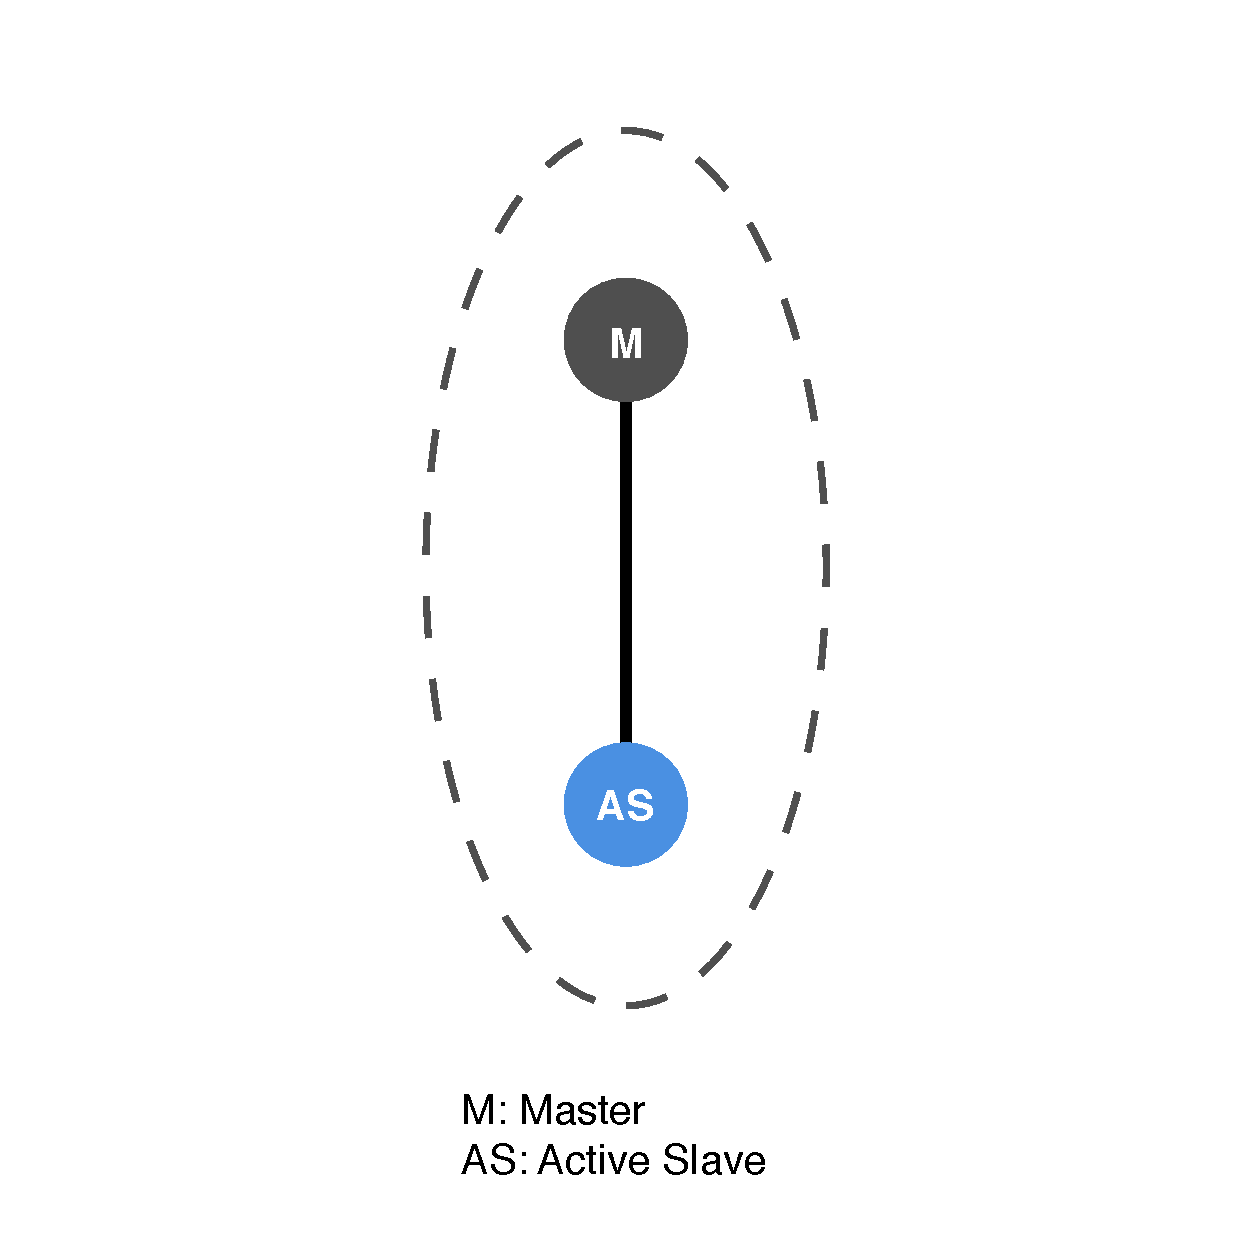
\includegraphics[width=7cm]{kapitel2/PicoNetz1.pdf}
\end{minipage}
\hfill
\begin{minipage}[hbt]{7cm}
  \centering
  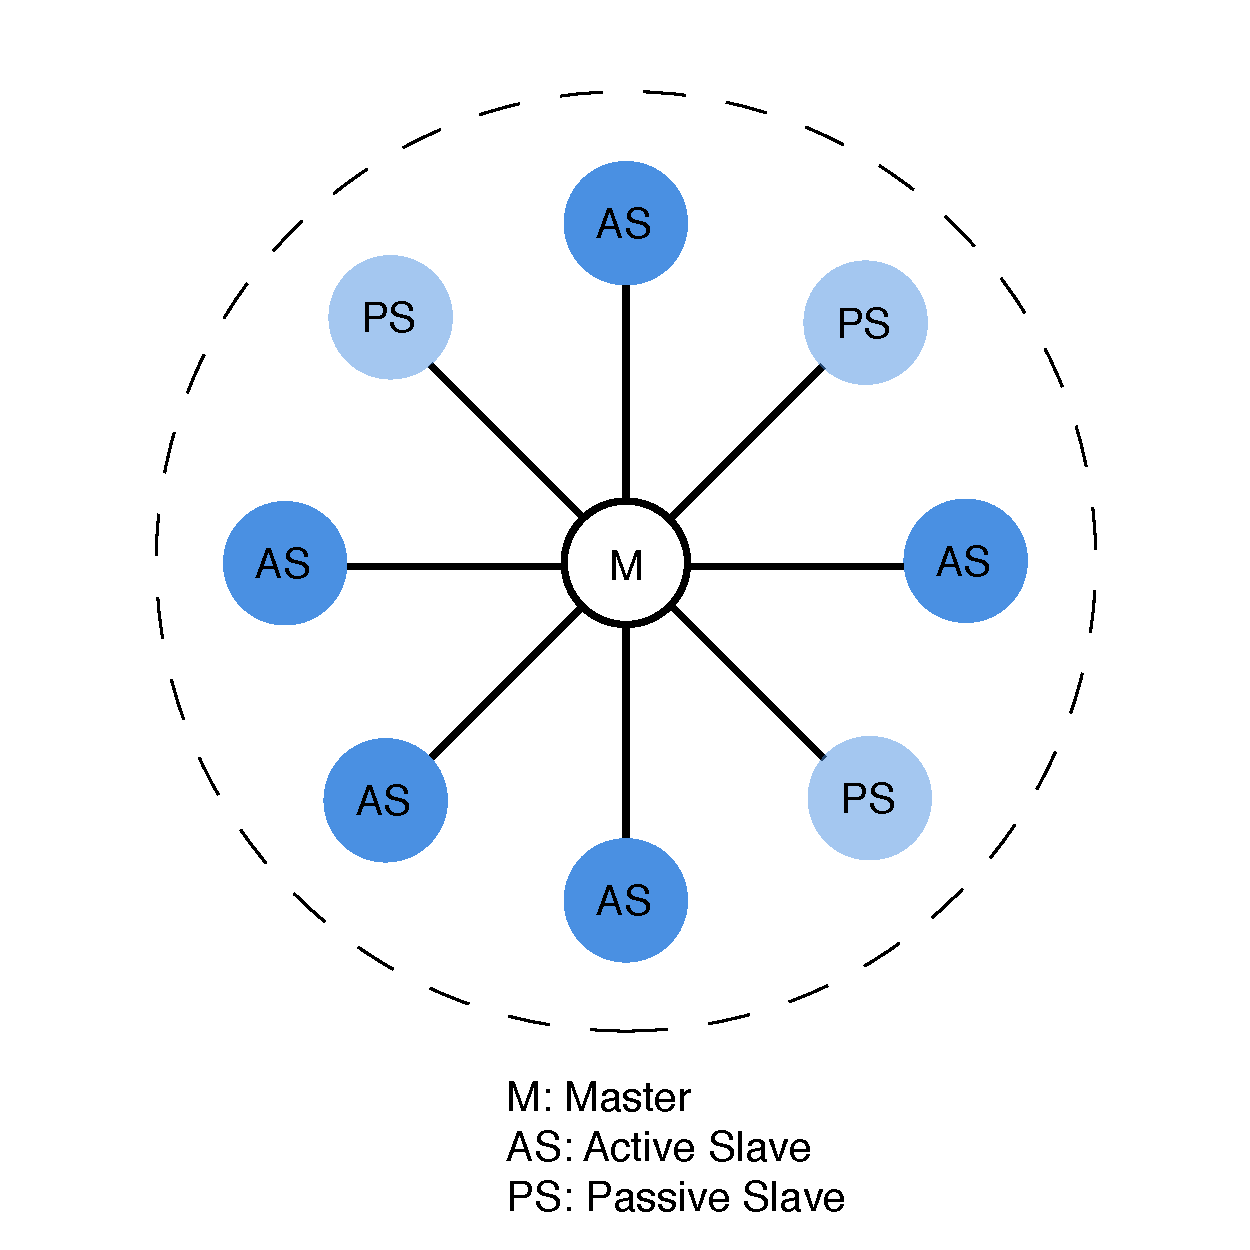
\includegraphics[width=7cm]{kapitel2/PicoNetz2.pdf}
\end{minipage}
\caption{Bluetooth-Topologie Piconetz \cite[vgl. Abb. 5.4]{baun2012computernetze}}
\label{fig:pico1}
\end{figure}

Bevor Daten übertragen werden können, müssen sich Geräte erst über den Vorgang des Pairings kennen lernen. Bei diesem Vorgang müssen die Benutzer jeweils einen gemeinsamen Code durch Tastendruck auf ihrem Gerät bestätigen. Nachdem Geräte einmal gepaired wurden, ist ein weiteres Pairing nicht mehr nötig, da sie sich bereits kennen. Seit Version 3.0 beherrscht Bluetooth den High Speed Modus, welcher eine Kombination aus Bluetooth und \ac{WLAN} 802.11g ist. Über die Bluetooth Verbindung mit 3 Mbit/s werden dabei nur noch Steuerdaten sowie Sitzungsschlüssel übertragen. Für die Nutzdaten wird eine Ad-hoc Verbindung über \ac{WLAN} aufgebaut, die eine Datentransferrate von ca 24 Mbit/s erreicht \cite[55-57]{baun2012computernetze}.

\subsubsection{NFC} 
Near Field Communication auch als \ac{NFC} bekannt, ist eine Funktechnologie für sehr kurze Distanzen. In einer Reichweite von optimal 4 cm und maximal  20 cm können Geräte miteinander eine Peer to Peer Verbindung eingehen und Daten mit bis zu 424 kBit/s übertragen. Anders als bei \ac{WLAN} und Bluetooth ist es mit \ac{NFC} nicht möglich, Verbindungen zu mehreren Geräten gleichzeitig zu unterhalten. Einen weiteren Unterschied stellt der Verbindungsaufbau zwischen den Geräten dar. Dieser ist bei \ac{NFC} sehr einfach gestaltet, da das Pairing allein durch die unmittelbare Nähe der Geräte zueinander geschieht und keine weiteren Aktionen des Nutzers benötigt. Aus diesem Grund wird \ac{NFC} auch in Verbindung mit Bluetooth oder \ac{WLAN} genutzt um schnell und einfach eine Verbindung aufzubauen ohne Passworteingabe bei \ac{WLAN} oder Code Bestätigung bei Bluetooth \cite{agrawal2012near}. \ac{NFC} ist verfügbar auf Android- und Windows-Geräten. Obwohl \ac{NFC} ab dem iPhone 6 integriert ist, sind keine \acs{API}s für Entwickler vorhanden. 

\subsubsection{Mobilfunk}
Moderne Mobilfunknetze bieten neben dem Zugang zu Telefondiensten auch Zugang zu Internetdiensten. Die aktuellsten Mobilfunkstandards sind \ac{HDSPA+} und \ac{LTE}. Bei \ac{HDSPA+} handelt es sich um eine Erweiterung des Mobilfunkstandards \acs{UMTS} mit Datenraten von bis zu 42 Mbit/s \cite{HDSPA:Online}. \ac{LTE} dagegen ist eine komplett neu entwickeltes Mobilfunknetz, das in der aktuellen Spezifikation theoretische Datenraten von bis zu 75 Mbit/s im Upload und 300 Mbit/s im Download bietet \cite{LTE:Online}.

\subsection{Datenkommunikation zwischen mobilen Endgeräten}
Über die Technologien, die im vorherigen Abschnitt beschrieben wurden, kann abhängig von der Technologie, entweder direkt zwischen Geräten im Netzwerk oder über einen Server kommuniziert werden. Folgend wird beschrieben, mit welchen Protokollen die Kommunikation in beiden Fällen umgesetzt werden kann. 

\subsubsection{Datenkommunikation in lokalen Netzwerken}
Sollen mobile Applikationen über ein lokales Netzwerk miteinander kommunizieren kann dies durch die Nutzung von Netzwerkdiensten realisiert werden. Ein Netzwerkdienst ist ein Informationsobjekt, das von einer Person, einem Programm, oder von einem anderen Dienst genutzt werden kann. Jeder Dienst stellt eine Funktionalität zur Verfügung, dabei kann es sich z.B. um Anwendungsdienste oder Kommunikationsdienste handeln \cite{cheng2002service}.  Eine wichtige Komponente zur Nutzung von Diensten ist \textit{service discovery}, über welches angebotene Dienste in einem Netzwerk gefunden werden können. Für service discovery existieren verschiedene Protokolle. Apple nutzt in seinen Betriebssystemen Bonjour \cite{AboutBonjour:Online}, Android nutzt Network Service Discovery \cite{AndroidDiscovery:Online}, um nur zwei Vertreter zu nennen. Beide Protokolle ermöglichen das automatische entdecken von Geräten und Diensten in lokalen Netzwerken.

Ein Dienst wird unter Anderem durch seinen Namen beschrieben. Dieser Name ist im Netzwerk sichtbar für alle Geräte, die danach suchen. Angebotene Dienste sollten einen einzigartigen Namen aufweisen, um Konflikte zwischen verschiedenen Applikationen zu vermeiden. Durch den Einsatz von Diensten können verschiedene Applikationen in einem Netzwerk untereinander kommunizieren. Dabei ist die Topologie des Netzwerkes unerheblich. Netzwerkdienste können in Infrastrukturnetzwerken (Siehe Abbildung \ref{fig:diensteGrund} a) genutzt werden und auch um Ad-Hoc Netzwerke zu bilden (Siehe Abbildung \ref{fig:diensteGrund} b).

\begin{figure}[H]
  \centering
  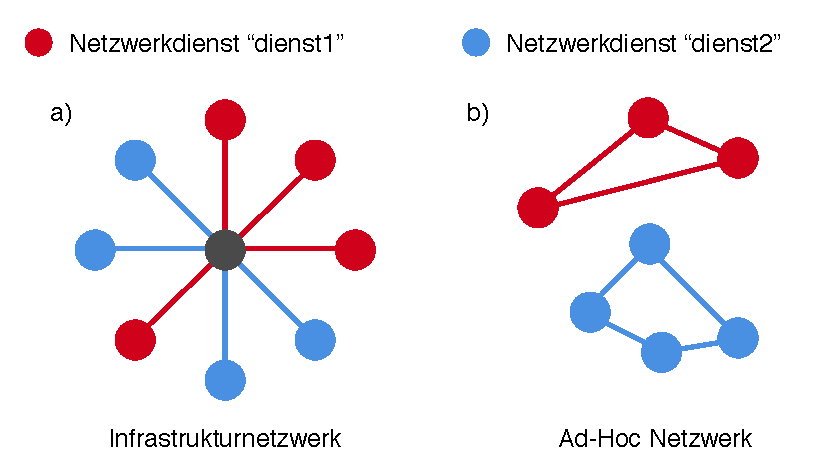
\includegraphics[width=\linewidth]{kapitel2/netzwerkdiensteGrundlagen.pdf}
  \caption{Netzwerkdienste in Computernetzwerken}
  \label{fig:diensteGrund}
\end{figure}

\subsubsection{Datenkommunikation über einen Server}
Anstatt direkt in einem lokalen Netzwerk zu kommunizieren, können Applikationen auch über einen Server Daten austauschen. Das Standardmodell für diese Kommunikation ist das Client-Server-Modell (Siehe Abbildung \ref{fig:clientServer}). In diesem Modell rufen Clients bestimmte Funktionalitäten bzw. Dienstleistungen, die ein Server zur Verfügung stellt, über ein Netzwerk hinweg auf \cite[14]{schill2012verteilte}.  
\begin{figure}[H]
  \centering
  \includegraphics[width=10cm]{kapitel2/clientServer.pdf}
  \caption{Client-Server-Modell}
  \label{fig:clientServer}
\end{figure}
\subsubsection{HTTP Operationen}
Clients stehen \acs{HTTP} Operationen zur Verfügung, mit denen die Kommunikation mit einem Server erfolgen kann. Die wichtigsten dieser Operationen \cite[14]{rodriguez2008restful}, sind die sogenannten \acs{CRUD} Operationen: create, read, update and delete. Die entsprechenden \acs{HTTP} Methoden, mit denen diese Operationen durchgeführt werden können, sind:
\begin{itemize}
\item POST um Ressourcen auf dem Server anzulegen.
\item GET um Ressourcen aufzurufen.
\item PUT um eine Recource zu aktualisieren
\item DELETE um eine Recource zu löschen
\end{itemize}
Endgeräte tauschen über diese Methoden Daten aus, indem eines der Geräte eine Ressource auf dem Server anlegt, während das andere Gerät die entsprechende Ressource aufruft. Der Datenaustausch über diese Methoden hat zur Folge, dass Clients anhaltend überprüfen müssen, ob die Daten bereits auf dem Server verfügbar sind. Für mobile Endgeräte ist dieser Vorgang aber nachteilig, da die ständigen Anfragen an den Server kostbare Batterielaufzeit verschwenden \cite{lando2007efficient}. Es existiert jedoch eine alternative Möglichkeit, mit der Client und Server kommunizieren können ohne dieses Problem, in der Form von Web Sockets.

\subsubsection{Web Sockets}
Web Sockets ermöglichen eine bidirektionale Verbindung zwischen einer Anwendung und einem Webserver. Wurde einmal eine Socket Verbindung durch den Client geöffnet, kann diese Verbindung aus beiden Richtungen verwendet werden. Für einen Datenaustausch bedeutet dies, dass Endgeräte nicht konstant nachfragen müssen, ob eine Ressource vorhanden ist. Der Server sendet die Daten selbstständig an die Clients, sobald Sie verfügbar sind. Socket-Verbindungen bleiben dauerhaft bestehen und werden erst geschlossen, wenn der Client die Verbindung schließt \cite{lubbers2010html5}.



\subsection{Technologien zur Geräteortung}

\subsubsection{GPS}
\label{subsec:GPS}
Das Global Positioning System \ac{GPS} ist ein globales mit Satelliten betriebenes Navigationssystem zur Positionsbestimmung. Ist ein Endgerät mit \ac{GPS} ausgestattet, ist es möglich, den Standort dieses Geräts zu bestimmen. Der Standort wird in geographische Koordinaten angegeben, mit denen sich die Lage eines Punktes auf der Erde beschreiben lässt \cite{wiki:GPS}. Die Funktionsfähigkeit von \ac{GPS} ist maßgeblich von der Empfangsqualität abhängig, so ist eine Ortung in Gebäuden häufig nicht möglich und auch die Genauigkeit der Positionsbestimmung kann negativ beeinflusst werden. In der Regel wird \ac{GPS} in Kombination mit anderen Technologien wie Mobilfunk-, \ac{WLAN}- oder Bluetooth genutzt. Dadurch kann zum einen der Verbindungsaufbau zu den Satelliten beschleunigt und zum anderen die Genauigkeit der Standortbestimmung verbessert werden. Trotz dieser Technik unterliegen die mit \ac{GPS} ermittelten Standortdaten häufig einer Ungenauigkeit die mehrere Meter hoch ausfallen kann \cite{AppleLocationServices:Online}.

\subsubsection{iBeacon}
\label{subsec:beacons}
Mit iBeacon können standortbezogene Dienste und Navigationslösungen in geschlossenen Räumen realisiert werden. iBeacon ist Apple's Markenname für eine Technologie, die Teil des Bluetooth Low Energy Standards ist. Dadurch ist iBeacon auf allen Endgeräten verfügbar die über Bluetooth LE verfügen und deren Betriebssystem kompatibel ist. Momentan sind das \acs{iOS}7 und Android 4.3. Neben Software Komponenten umfasst die Beacon Technologie auch Hardware Komponenten. Dies sind speziell entwickelte Signalgeber, ebenfalls als iBeacons oder Beacons bezeichnet, die mit Bluetooth LE Technik ausgestattet sind. Diese Hardware Beacons werden jedoch nicht in allen Anwendungsszenarien benötigt, da jedes kompatible Smartphone ebenfalls die Funktionen eines Beacons übernehmen kann \cite{wiki:iBeacon}.

iBeacon unterscheidet drei Grundlegende Funktionen: \textit{Advertising}, \textit{Ranging} und \textit{Region Monitoring}. Im folgenden werden diese Funktionen beschrieben und die Funktionsweise der Beacon Technologie dargestellt.

\paragraph{Advertising}
ist der Vorgang mit dem Beacons andere Geräte über ihre Anwesenheit informieren. Jedes Beacon spannt einen Bereich um sich, der als \textit{region} bezeichnet wird. Innerhalb dieses Aktionsradius senden Beacons kontinuierlich Signale mit Informationen über ihre Identität aus.

Die Identität eines Beacons setzt sich zusammen aus einer 16 Byte \textit{\acs{UUID}} (\acl{UUID}) sowie einem \textit{major} und einem \textit{minor} Wert die jeweils 2 Byte groß sind. Die \textit{\acs{UUID}} ist ein Identifikator der je nach Anwendungsfall von einem oder mehreren Beacons genutzt werden kann. Mit \textit{major} und \textit{minor} Wert kann für jedes Beacon eine einzigartige ID gebildet werden mit der dieses eindeutig aus einer Gruppe von Beacons mit der selben \textit{\acs{UUID}} identifiziert werden kann (Siehe Abbildung \ref{fig:beaconRegion}).

\begin{figure}[H] 
\centering 
  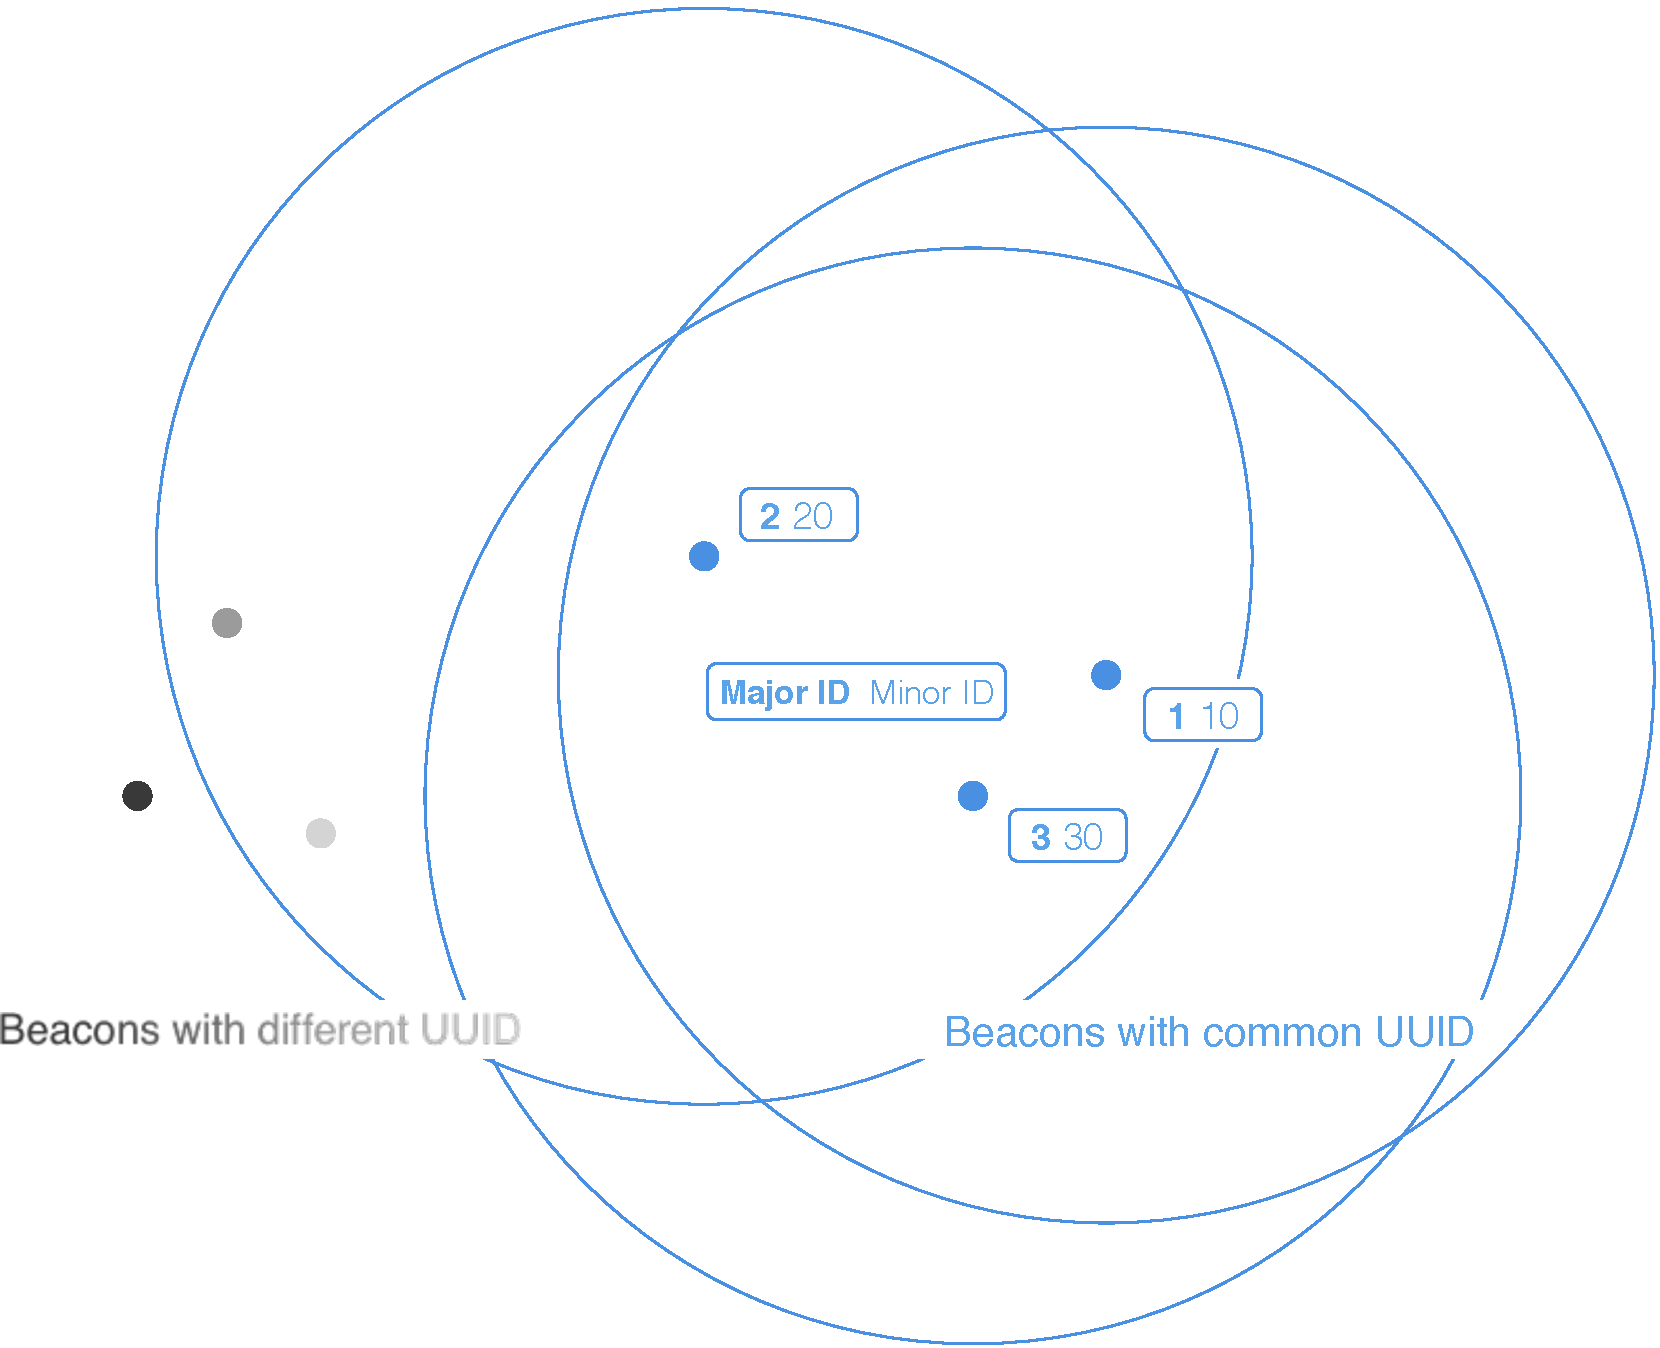
\includegraphics[width=\linewidth]{kapitel2/beaconRegions.pdf}
  \caption{iBeacon regions}
  \label{fig:beaconRegion}
\end{figure}

Die folgende Tabelle zeigt ein Beispiel wie die Werte genutzt werden können um iBeacons in einer Einzelhandelskette einzusetzen.

\begin{table}[H]
\centering
\begin{tabular}{| >{\centering\arraybackslash}m{1.5cm} | >{\centering\arraybackslash}m{2cm} | >{\centering\arraybackslash}m{2,8cm} | >{\centering\arraybackslash}m{2,8cm} | >{\centering\arraybackslash}m{2,8cm} |}
\hline
\multicolumn{2}{|c|}{\cellcolor[HTML]{C0C0C0}Store Location}  & \cellcolor[HTML]{C0C0C0}San Francisco & \cellcolor[HTML]{C0C0C0}Paris & \cellcolor[HTML]{C0C0C0}London\\
\hline
\multicolumn{2}{|c|}{\cellcolor[HTML]{EFEFEF}UUID}  & \multicolumn{3}{c|}{D9B9EC1F-3925-43D0-80A9-1E39D4CEA95C}\\
\hline
\multicolumn{2}{|c|}{\cellcolor[HTML]{EFEFEF}Major} & 1 & 2 & 3\\
\hline
\cellcolor[HTML]{EFEFEF} & \cellcolor[HTML]{EFEFEF}Clothing & 10 & 10 & 10\\
\cline{2-5}
\cellcolor[HTML]{EFEFEF}Minor & \cellcolor[HTML]{EFEFEF}Housewares & 20 & 20 & 20\\
\cline{2-5}
\cellcolor[HTML]{EFEFEF} & \cellcolor[HTML]{EFEFEF}Automotive & 30 & 30 & 30\\
\hline
\end{tabular}
\caption{Einsatz von Beacons in einer Einzelhandelskette \cite{iBeacon:2014}}
\label{tableBeacon}
\end{table}

In diesem Beispiel wird die \textit{\acs{UUID}} von den Beacons an allen Standorten gemeinsam genutzt und Identifiziert die Handelskette als ganzes. Jede Filiale wird durch einen \textit{major} Wert identifiziert. Innerhalb einer jeden Filiale werden die einzelnen Abteilungen durch einen \textit{minor} Wert repräsentiert. Mit Hilfe dieser Informationen ist eine Applikation in der Lage festzustellen, ob der Benutzer eine der Filialen betritt, verlässt und in welcher Abteilung er sich gerade befindet \cite{iBeacon:2014}.

\paragraph{Ranging}
ist die Funktion mit der eine Applikation nach Signalen sucht die von Beacons ausgesendet werden. Es können dabei nur Signale empfangen werden von Beacons deren \textit{\acs{UUID}} der Applikation bekannt sind. Werden zum ersten mal Signale eines solchen Beacons empfangen, wurde die \textit{region} dieses Beacons betreten und ein Event wird in der Applikation ausgelöst. Umgekehrt bedeutet der langfristige Verlust des Beacon-Signals, dass die \textit{region} verlassen wurde. Wie beim Betreten, wird auch beim Verlassen einer \textit{region} ein entsprechendes Event in der Applikation ausgelöst \cite{iBeacon:2014}.

Nachdem eine \textit{region} betreten wurde, kann der Abstand zum Beacon anhand der Signalstärke \textit{\acs{RSSI}} (\acl{RSSI}) näherungsweise bestimmt werden. Die Ermittlung des Abstands ist anfällig, ungenaue Ergebnisse zu produzieren da das Signal durch externe Faktoren beeinflusst werden kann \cite{EstimoteBeaconSignal:Online}. Bei diesen Faktoren kann es sich sowohl um Räumliche Begebenheiten handeln als auch um Interferenzen die durch andere Funksignale z.B. durch WLAN ausgelöst werden können. Der iBeacon Hersteller Estimote ermittelte in internen Tests Abweichungen von 5-6cm bei einem Abstand von 20cm sowie 2-3m bei Abständen von über 10m \cite{EstimoteBeaconSignal:Online}. Die Genauigkeit der Messung scheint also fundamental vom Abstand zu Beacons bzw.  der Signalstärke abzuhängen. Um Entwicklern eine Möglichkeit zu geben, auf Ungenaue Messergebnisse zu reagieren, gibt \acs{iOS} eine Einschätzung zur Genauigkeit der Messung mit dem \textit{accuracy} Parameter aus. Ist der \textit{accuracy} Wert niedrig bedeutet dies, dass sich \acs{iOS} sehr sicher ist über die Genauigkeit der Messung. Umgekehrt bedeutet ein hoher \textit{accuracy} Wert, dass der ermittelte Abstand sehr wahrscheinlich ungenau ist \cite{iBeacon:2014}.

Ist für ein Anwendungsszenario eine ungefähre Abschätzung über den Abstand zu einem Beacon ausreichend, kann man diese über die vier vordefinierten \textit{proximity states} erhalten. Diese lauten: \textit{unknown}, \textit{far}, \textit{near} und \textit{immediate}. \textit{Unknown} beschreibt dabei die Entfernung, die ermittelt wird, sollte sich das Smartphone außerhalb der Reichweite des Beacons befinden oder sollte die Qualität der empfangenen Signale nicht ausreichen, um den Abstand festzustellen. Wird \textit{far} als Abstand ausgegeben, werden Beacon Signale empfangen, jedoch sind Sie schwach oder \acs{iOS} ist sich unsicher über die Genauigkeit der Messung. Der Abstand zum Beacon kann zwischen 70m und 3m liegen. \textit{near} beschreibt eine Zone in der die Signalstärke gut ist und die Genauigkeit ebenfalls als gut eingeschätzt wird. Der Abstand zum Beacon bewegt sich zwischen 0.5m und 3m. Der letzte mögliche \textit{proximity state} ist \textit{immediate}. Wird dieser Status angezeigt ist die Signalstärke sehr hoch und \acs{iOS} ist sich sehr sicher über die Genauigkeit der Messung. Der Empfänger befindet sich in einem Abstand von unter 0.5m zum Sender (Siehe Abbildung \ref{fig:beaconRegion}). In einer Applikation wird für jeden der \textit{proximity state} ein entsprechendes Event ausgelöst sobald dieser festgestellt wird \cite{EstimoteBeaconSignal:Online}.

\begin{figure}[H] 
\centering 
  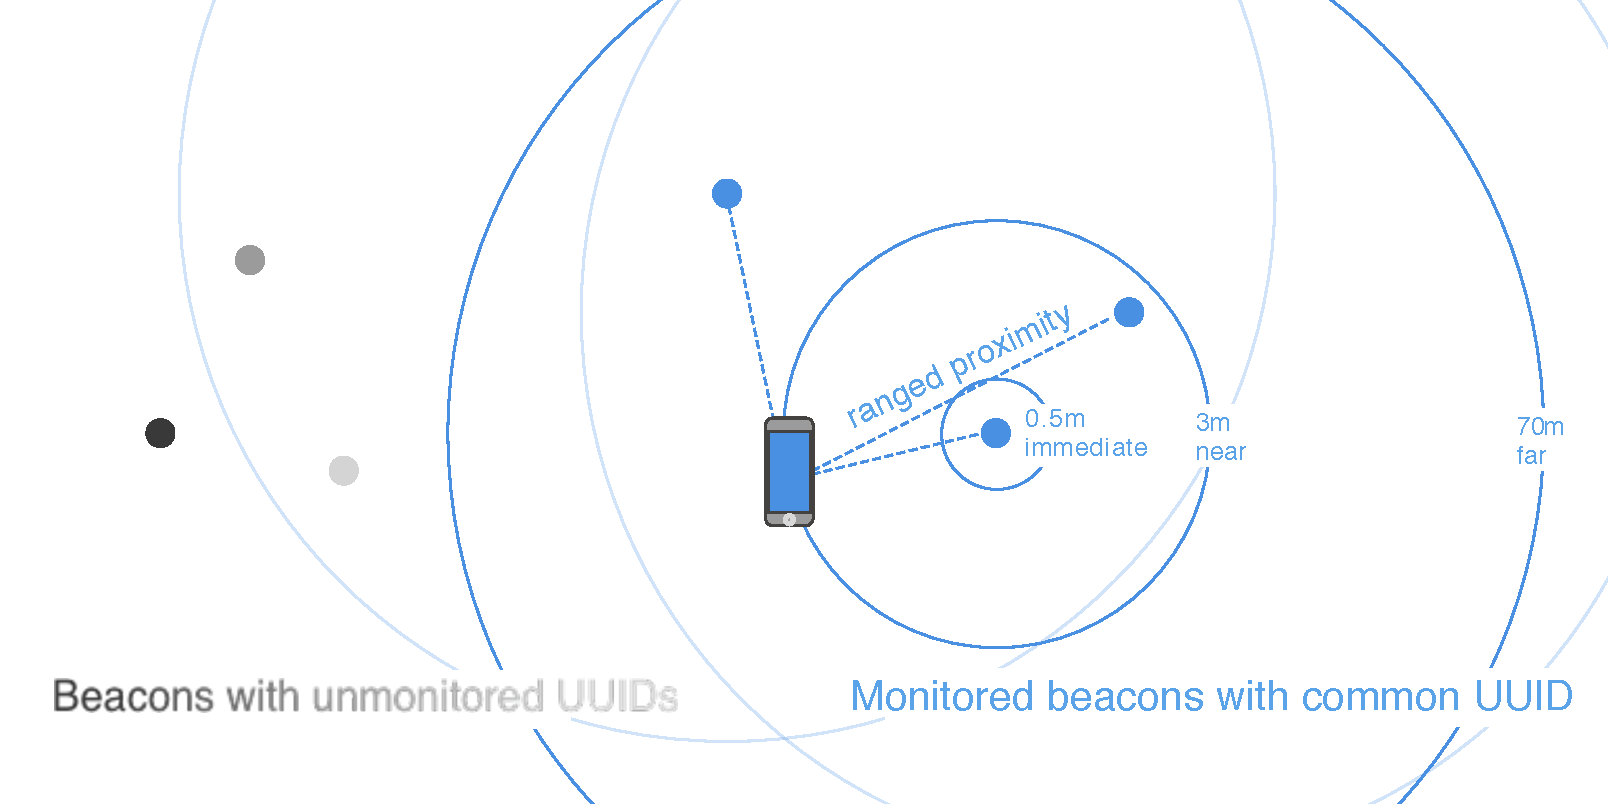
\includegraphics[width=\linewidth]{kapitel2/beaconRanging.pdf}
\caption{iBeacon ranging} 
\end{figure}

\paragraph{Region Monitoring} bietet eine weitere Funktionalität mit der Applikationen Events auslösen können sobald das Smartphone eine definierte Beacon \textit{region} betritt oder verlässt. Dafür muss die Bump-Applikation im Gegensatz zur selben Funktionalität beim \textit{Ranging} nicht aktiv sein. Geschlossene Applikationen können durch das \textit{Region Monitoring} im Hintergrund gestartet werden und z.B. \textit{Push Notifications} auslösen. Andere Aktionen die ausgeführt werden können, während eine Applikation im Hintergrund ist, sind auch möglich.

\subsection{Sensoren}
Mobile Endgeräte sind mit einer Reihe von Sensoren ausgestattet, mit denen es möglich ist, unentwegt Daten zu sammeln. Applikationen können diese Daten auswerten, um zu sehen, hören und fühlen, was mit dem Gerät und in seiner Umgebung geschieht. Bewegungen des Anwenders bzw. des Endgeräts können durch die Auswertung der Daten des Beschleunigungssensors erkannt werden. Ein Beschleunigungssensor, auch Accelerometer genannt, ist ein Sensor, mit dem Beschleunigung oder g-Kraft in Meter pro Quadratsekunde ($m/m^{2}$) gemessen werden kann. In mobilen Endgeräten sind in der Regel drei Sensoren eingebaut, mit denen die Beschleunigung auf x, y und z-Achse bestimmt werden kann (Siehe Abbildung \ref{fig:Beschleunigungssensor}). Durch die Auswertung der Sensordaten können Bewegungen des Benutzers z.B. laufen, rennen oder Treppensteigen erkannt werden. Die Daten können aber auch genutzt werden, um zu erkennen, ob sich ein Endgerät im freien Fall befindet, oder um Erschütterungen festzustellen, wenn das Gerät gegen etwas stößt \cite{ravi2005activity}. 

\begin{figure}[H]
    \centering
    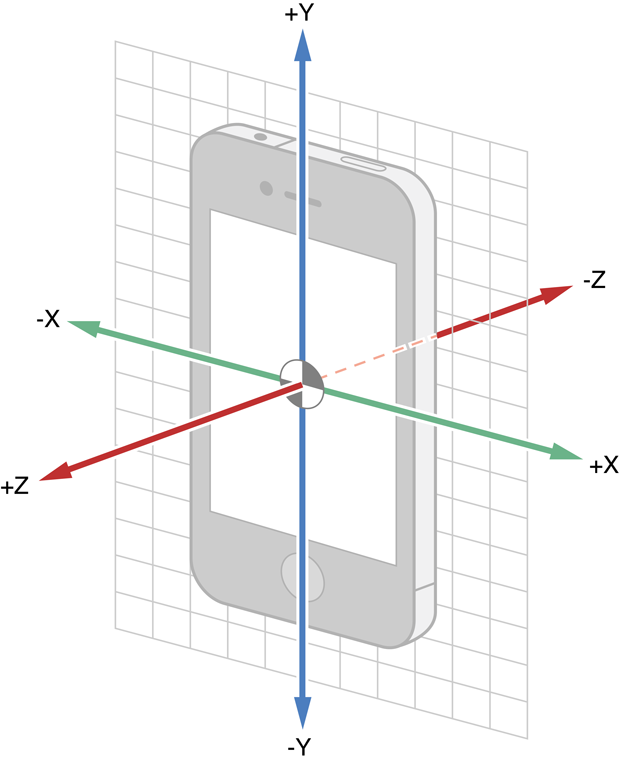
\includegraphics[width=0.4\textwidth]{kapitel2/Accelerometer.png}
    \caption{3-Achsen Beschleunigugnssensor \cite{AppleAccelerometer:Online}}
    \label{fig:Beschleunigungssensor}
\end{figure} % Externe Datei einbinden
\chapter{Analyse der Bump-Geste}
\label{Kap3}
\label{chap:Kap3}

Bei der Bump-Geste handelt es sich um eine Interaktion bei der von einem Quellgerät, auf dem ein Anwender eine Aktivität begonnen hat, Daten durch einen Bump auf ein Zielgerät übertragen werden, damit der Anwender auf diesem seine Aktivität fortsetzen kann. Um genau zu klären, wie dieser Vorgang funktioniert, wird in diesem Kapitel untersucht, wie die Interaktion abläuft, in welchen Varianten die Geste durchgeführt werden kann, welche Endgeräte sich für die Geste eignen und wie die Geste in einer Applikation umgesetzt werden kann.

\section{Ablauf der Interaktion}
Die Interaktion kann aufgeteilt werden in die Aktionen des Benutzers und die Reaktion der Systeme auf die Interaktion.

\subsection{Aktionen des Benutzers}
Wird die Interaktion zwischen zwei Anwendern durchgeführt, halten beide Benutzer jeweils ein Gerät fest in der Hand und lassen die Geräte zusammenstoßen/bumpen. Erfolgt die Interaktion zwischen einem Anwender und einem stationären Endgerät hält entsprechend ein Anwender sein Gerät fest in der Hand und lässt es auf das stationäre Gerät bumpen.

\begin{figure}[H]
    \centering
    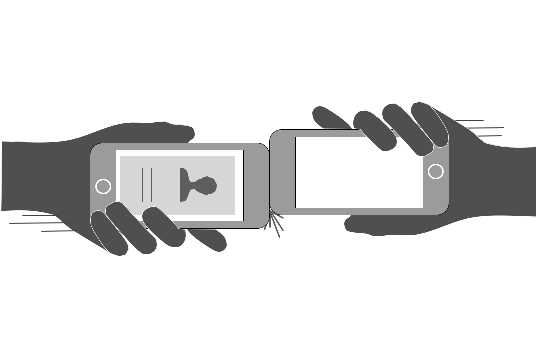
\includegraphics[width=6cm]{kapitel4/Bump.pdf}
    \label{actionUser}
\caption{Aktion des Benutzers}
\end{figure}


\subsection{Reaktion des Systems}
Die hauptsächliche Reaktion des Systems ist es, die Daten des Quellgeräts auf das Zielgerät zu übertragen und dort anzuzeigen (Siehe Abbildungen \ref{fig:transfer}, \ref{fig:anzeigen}). Die Geräte sollten aber auch eine visuelle oder akustische Rückmeldung an die Benutzer geben, um zu signalisieren, dass ein Bump von den Endgeräten festgestellt wurde, z.B. über Vibration und mit welchem Gerät/Person Daten ausgetauscht werden. 

\begin{figure}[H]
\begin{minipage}[h]{7cm}
    \centering
    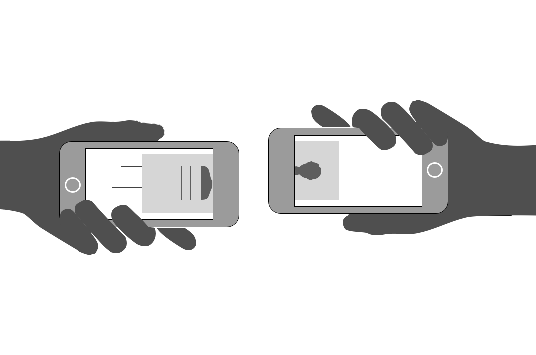
\includegraphics[width=6cm]{kapitel4/Transfer.pdf}
    \caption{Daten übertragen}
    \label{fig:transfer}
\end{minipage}
\hfill
\begin{minipage}[h]{7cm}
    \centering
    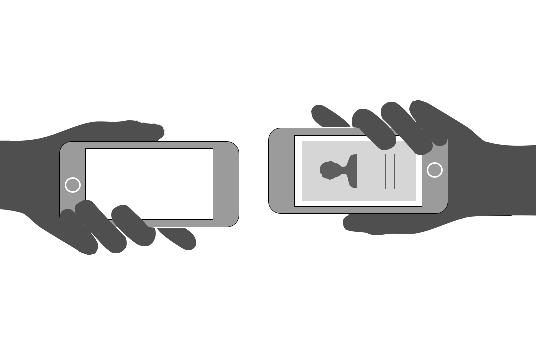
\includegraphics[width=6cm]{kapitel4/Complete.pdf}
    \caption{Daten anzeigen}
    \label{fig:anzeigen}
\end{minipage}
\end{figure}

\section{Variationen der Bump-Geste}
Die Bump-Geste lässt sich auf verschiedene Art und Weisen durchführen. An dieser Stelle sollen einige dieser Variationen als Beispiel dienen, um zu illustrieren wie eine Bump-Geste aussehen kann.

\begin{tabular}{p{5cm} p{8cm}}
    \vspace{0pt} 
    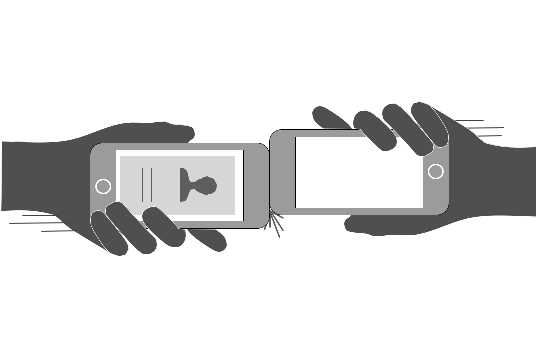
\includegraphics[width=4cm]{kapitel4/Bump.pdf}
    \begin{minipage}[h]{4cm}
        \captionof{figure}{Stirnseite an Stirnseite}    
    \end{minipage}
    & 
    \vspace{-3ex}
    \subsubsection{Stirnseite an Stirnseite}
    Die Endgeräte werden waagerecht in den Händen der Anwender gehalten und werden an den Stirnseiten zusammengestoßen.
\end{tabular}


\begin{tabular}{p{5cm} p{8cm}}
    \vspace{0pt} 
    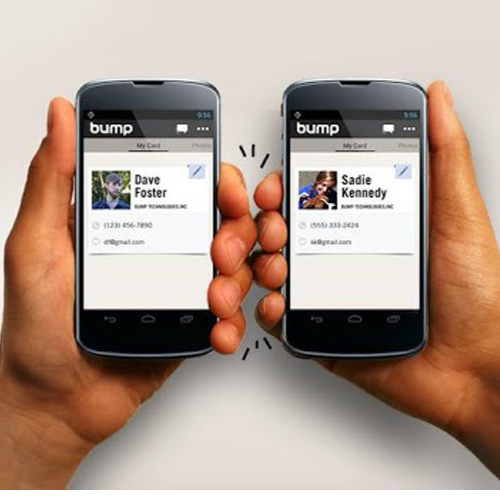
\includegraphics[width=4cm]{kapitel2/bumpPhone.png}
    \begin{minipage}[h]{4cm}
        \captionof{figure}{Längsseite an Längsseite}
    \end{minipage}
    & 
    \vspace{-3ex}
    \subsubsection{Längsseite an Längsseite}
    Die Endgeräte werden aufrecht in den Händen der Anwender gehalten und werden an den Längsseiten zusammengestoßen. Dabei können die Geräte auch von den Händen umschlossen werden wodurch die Interaktion wie ein Fistbump aussieht.
\end{tabular}


\begin{tabular}{p{5cm} p{8cm}}
    \vspace{0pt} 
    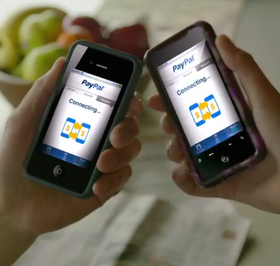
\includegraphics[width=4cm]{kapitel3/bumpEcke.png}
    \begin{minipage}[h]{4cm}
        \captionof{figure}{Ecke an Ecke}
    \end{minipage}
    & 
    \vspace{-3ex}
    \subsubsection{Ecke an Ecke}
    Die Endgeräte werden aufrecht in den Händen der Anwender gehalten und werden an den oberen Ecken zusammengestoßen.
\end{tabular}

\begin{tabular}{p{5cm} p{8cm}}
    \vspace{0pt}
    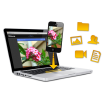
\includegraphics[width=4cm]{kapitel3/bumpLaptop.png}
    \begin{minipage}[h]{4cm}
        \captionof{figure}{Stirnseite aufstoßen}
    \end{minipage}
    & 
    \vspace{-3ex}
    \subsubsection{Stirnseite aufstoßen} 
    Ein Endgerät wird vom Anwender aufrecht in der Hand gehalten und mit der oberen oder unteren Kante auf ein stationäres Gerät (SurfaceTable, Notebook) aufgestoßen.
\end{tabular}

\section{Geeignete Endgeräte}
Aus den dargestellten Bump-Variationen ist zu erkennen, das die Bump-Interaktion zwischen verschiedenen Typen von Geräten erfolgen kann. Es gilt an dieser Stelle allgemein zu klären, zwischen welchen Geräteklassen die Bump-Geste eingesetzt werden kann. Die Geräte werden nach Terrenghi et al. \cite{Terrenghi:2009:TAM:1644246.1644265} basierend auf ihrer Bildschirmgröße kategorisiert. Die folgende Tabelle liefert einen Überblick über diese Kategorien.

\begin{table}[H]
\begin{tabular}{| >{\arraybackslash}m{4.2cm} | >{\centering\arraybackslash}m{4.2cm} | >{\centering\arraybackslash}m{4.2cm} |}
\hline
\cellcolor[HTML]{C0C0C0}Kategorie   & \cellcolor[HTML]{C0C0C0} Bildschirmgröße &  \cellcolor[HTML]{C0C0C0} Beispiel       \\ \hline
Inch size                           &  $\ge$  2,54 cm                            &  Smartphone                             \\ \hline
\cellcolor[HTML]{EFEFEF}Foot size   &  \cellcolor[HTML]{EFEFEF}  $\ge$ 30,48 cm    &  \cellcolor[HTML]{EFEFEF}Tablet         \\ \hline
Yard size                           &  $\ge$ 91,44 cm                          &  Tabletop                               \\ \hline
\cellcolor[HTML]{EFEFEF}Perch size  &  \cellcolor[HTML]{EFEFEF}  $\ge$   05 m     & \cellcolor[HTML]{EFEFEF} TV-Bildschirm  \\ \hline
Chain size                          &  $\ge$   20 m                              &  Mehrere Displays                       \\ \hline
\end{tabular}
\caption{Kategorisierung von Endgeräten}
\label{kategory}
\end{table}


Um für die Interaktion geeignete Geräte zu identifizieren gilt es erst zu definieren welche verschiedenen Rollen ein Gerät in der Interaktion einnehmen kann. Die Endgeräte können aufgeteilt werden in Quell- und Zielgeräte. Ein Quellgerät ist der Informationsträger, von welchem Daten durch den Bump auf das Zielgerät übertragen werden. Bei einem Quellgerät muss es sich um ein mobiles Endgerät handeln. Es muss vom Anwender einfach in einer oder zwei Händen gehalten, bewegt und auf das Zielgerät gestoßen werden können. Bei Zielgeräten hingegen kann es sich sowohl um ein mobiles als auch um ein stationäres Endgerät handeln. Stationäre Endgeräte zeichnen sich dadurch aus, dass Sie vom Anwender bei der Nutzung nicht in der Hand gehalten werden.

Die definierten Gerätekategorien können jetzt auf die jeweiligen Rollen aufgeteilt werden. Quellgeräte können nur Geräte aus den Kategorien Inch size und Foot size sein. Zielgeräte können zusätzlich auch aus den Kategorien Yard-, Perch- und Chain size kommen.

Nachdem die Gerätekategorien zugeordnet sind gilt, es noch zu klären, ob die Geräte aus diesen Kategorien auch für die Interaktion geeignet sind. Inch und Foot size Geräte eignen sich für die Interaktion. Sie können vom Anwender einfach geführt werden und sowohl als Quell- als auch als Zielgerät dienen. Yard size Geräte eignen sich als Zielgerät. Der Anwender kann sein mobiles Endgerät auf das Gerät aufstoßen und kann sehen, welche Auswirkungen die Interaktion auf das Zielgerät hat. Für Perch- und Chain size Geräte gilt dies nicht, da ihre Bildschirme so groß sind und der Anwender für die Interaktion so nah an den Geräten stehen muss, dass er nicht sehen kann, was auf den Zielgeräten geschieht. Geräte aus diesen Kategorien eigenen sich daher nicht gut für die Bump-Geste. 

\section{Umsetzung der Interaktion}
Um die Bump-Interaktion umzusetzen, müssen drei Teilsysteme entwickelt werden: Eines dieser Systeme muss erkennen, wenn Endgeräte angestoßen werden. Ein weiteres System muss Endgeräte identifizieren können, damit die Daten zwischen den richtigen Geräten ausgetauscht werden. Außerdem wird ein System benötigt, über das ein Kommunikationskanal zwischen den Geräten hergestellt wird, über den Daten ausgetauscht werden können.
 % Externe Datei einbinden
\chapter{Umsetzung der Interaktion}
\label{Kap4}
\label{chap:Kap4}
Dieses Kapitel beschreibt Konzepte für die im vorangegangen Kapitel identifizierten Teilsysteme. Diese Konzepte beziehen sich zu einem großen Teil auf \acs{iOS} Frameworks, mit denen die Demonstrator Applikation entwickelt wurde. Aus diesem Grund werden diese Frameworks einleitend in Abschnitt \ref{sec:iOSFrameworks} beschrieben. Darauf folgt in Abschnitt \ref{sec:BumpErkennung} ein Konzept zur Erkennung von Bumps, in Abschnitt \ref{sec:Ident} werden Konzepte zur Identifizierung der Endgeräte beschrieben und in Abschnitt \ref{sec:Austausch} Konzepte zum Datenaustausch zwischen den Endgeräten.

\section{Grundlagen zu iOS Frameworks}
\label{sec:iOSFrameworks}
\acs{iOS} bietet durch Frameworks Zugang zu verschiedenen Technologien. Im folgenden wird die grundlegende Funktionsweise von drei Frameworks beschrieben, die zur Umsetzung der Bump-Interaktion genutzt wurden.

\subsection{Core Motion Framework}
\label{subsec:coreMotion}
Das Core Motion Framework bietet Applikationen Zugang zu Sensordaten die durch die Gerätehardware erfasst werden. Die Klasse \textit{CMMotionManager} ist die zentrale Anlaufstelle für den Zugriff auf alle Sensoren die Daten durch die Bewegung des Endgeräts erzeugen. Somit bietet sie auch Zugang zu den Daten des Beschleunigungssensors. Wird dieser konfiguriert ist die Variable \textit{accelerometerUpdateInterval} sehr wichtig.  

\begin{description}
  \item \textcolor{type}{var} \noindent\hspace*{1mm} accelerometerUpdateInterval: \textcolor{parameter}{NSTimeInterval}
        \\[2mm]
\end{description}

Die Variable legt das Intervall in Sekunden fest, in denen die Accelerometer-Daten aktualisiert werden und sollte dem Anwendungskontext entsprechend gewählt werden. Um Entwicklern Unterstützung zu bieten, die richtige Wahl zu treffen, bietet Apple die folgenden Empfehlungen \cite{AppleAccelerometer:Online}.

\begin{table}[H]
\begin{tabular}{|p{0.3\linewidth}|p{0.65\linewidth}|}
\hline
\cellcolor[HTML]{C0C0C0}Frequenz (Hz) & \cellcolor[HTML]{C0C0C0} Nutzung                                                                                                                                                                   \\ \hline
10–20                & Geeignet um die Ausrichtung des Geräts festzustellen.                                                                                                         \\ \hline
\cellcolor[HTML]{EFEFEF}30–60                & \cellcolor[HTML]{EFEFEF} Geeignet für Spiele und andere Applikationen die Eingaben des Benutzers in Echtzeit verarbeiten müssen.
                                                                                  \\ \hline
70–100               & Geeignet für Applikationen die Hochfrequente Bewegungen (Schütteln, Stöße) feststellen müssen.  \\ \hline
\end{tabular}
\caption{Beschleunigungssensor Aktualisierungsintervall \cite{AppleAccelerometer:Online}}
\label{accelerometerInterval}
\end{table}

Um die Daten des Sensors abzufragen, wird die Funktion \textit{accelerationUpdated} genutzt. Es handelt sich dabei um eine Callback-Funktion, die im festgelegten Intervall aufgerufen wird \cite{AppleAccelerometer:Online}.
\begin{description}
  \item \textcolor{type}{func} accelerationUpdated(accelerometerData: \textcolor{parameter}{CMAccelerometerData!}, error: \textcolor{parameter}{NSError!}) -> \textcolor{parameter}{Void}
        \\[2mm]
\end{description}


\subsection{Core Location Framework}
\label{subsec:coreLocation}
Das Core Location Framework bietet Zugriff auf die Technologien \acs{GPS} und iBeacon, mit denen standortbasierte Dienste realisiert werden können. Die Funktionsweise dieser Technologien wurde bereits in den Abschnitten \ref{subsec:beacons} und \ref{subsec:GPS} beschrieben. Dieser Abschnitt beschreibt für die Implementierung relevante Klassen und Protokolle.

Die zentrale Anlaufstelle für Ortungsdienste ist die Klasse \textit{CLLocationManager} und das dazugehörige Protokoll \textit{CLLocationManagerDelegate}. Werden \acs{GPS} Standortdaten gesucht, sind diese, sobald Sie verfügbar sind, über die Delegate-Methode \textit{didUpdateLocations} verfügbar.

\begin{description}
  \item \textcolor{type}{func} locationManager(manager: \textcolor{parameter}{CLLocationManager!}, didUpdateLocations: \textcolor{parameter}{[AnyObject]!})
\end{description}

Wird nach iBeacons gesucht, wird die Delegate-Methode \textit{didRangeBeacons} aufgerufen. Diese liefert ein Array mit allen gefundenen Beacons in Empfangsreichweite. Die Beacons in diesem Array sind sortiert nach ihrer gemessenen Entfernung, beginnend mit dem Beacon das die kürzeste Entfernung aufweist.

\begin{description} 
  \item \textcolor{type}{func} locationManager(manager: \textcolor{parameter}{CLLocationManager!}, didRangeBeacons: \textcolor{parameter}{[CLBeacon]!}, inRegion: \textcolor{parameter}{ CLBeaconRegion!})
\end{description}

\subsection{Multipeer Connectivity Framework}
Mit dem Multipeer-Connectivity-Framwork können \acs{iOS} und \acs{MacOS} Geräte über \ac{WLAN} oder Bluetooth kommunizieren. Dabei nutzen die Endgeräte jene Kommunikationskanäle, die verfügbar sind. Sind sie Teil eines Infrastrukturnetzwerkes, können Sie darüber Daten austauschen. Ist keine Verbindung zu solch einem Netzwerk vorhanden, wird je nachdem, welche Technologie bei den Kommunikationspartnern aktiviert, ist eine Ad-Hoc Verbindung über Bluetooth oder \ac{WLAN} aufgebaut \cite{AppleMultipeer:Online}.

Das Framework operiert in zwei Phasen, der \textit{Discovery Phase} und der \textit{Session Phase}. Diese werden folgend beschrieben.

\subsubsection{Discovery Phase}
In der Discovery Phase können sich Endgeräte, die in Empfangsreichweite zueinander sind, gegenseitig entdecken und eine Verbindung miteinander aufbauen. Mit den Klassen \textit{MCNearbyServiceAdvertiser} und \textit{MCNearbyServiceBrowser} können die Geräte Dienste anbieten und suchen. Um einen \textit{Advertiser} oder einen \textit{Browser} zu initialisieren müssen eine \textit{MCPeerID} und ein \textit{serviceType} als Parameter übergeben werden. Während die \textit{peerID} jedes Peer identifiziert, handelt es sich beim serviceType um einen bis zu 15 Zeichen langen Bezeichner, der bei allen Peers, die sie sich gegenseitig entdecken möchten, übereinstimmen muss \cite{AppleMultipeer:Online}.

\begin{description}
  \item \textcolor{class}{class} MCNearbyServiceAdvertiser(peer: \textcolor{parameter}{MCPeerID!}, discoveryInfo: \textcolor{parameter}{[NSObject : AnyObject!]}, serviceType: \textcolor{parameter}{String!})
  \item  \textcolor{class}{class} MCNearbyServiceBrowser(peer: \textcolor{parameter}{MCPeerID!}, serviceType: \textcolor{parameter}{String!})
\end{description}

Zusätzlich zu peerId und serviceType verfügt der MCNearbyServiceAdvertiser noch den optionalen Paramter \textit{discoveryInfo}. Dabei handelt es sich um ein \textit{dictionary}, in dem zusätzliche Informationen vom Advertiser an den Browser übermittelt werden können. Ein dictionary ist ein Datentyp bei dem Daten (\textit{values}) eines bestimmten Typs ungeordnet gespeichert werden. Diese können durch einen einzigartigen Bezeichner, auch \textit{key} genannt, referenziert und gesucht werden \cite{AppleCollectionTypes:Online}. Key und value des dictionarys müssen String Objekte sein und dürfen zusammen eine Größe von 255 Bytes nicht überschreiten. Für optimale Performance sollte das gesamte dictionary nicht größer als 400 Bytes sein, damit es in einem einzelnen Bluetooth Datenpaket untergebracht werden kann \cite{AppleMCNearbyServiceAdvertiser:Online}.

\subsubsection{Advertising und Browsing}
Startet ein Peer das Advertisement, wird dieses Peer für alle Browser in Empfangsreichweite sichtbar und teilt diesen Peers die Bereitschaft zum Verbindungsaufbau mit. Advertiser in Empfangsreichweite werden dem Browser über die Delegate Methode \textit{foundPeer} des \textit{MCNearbyServiceBrowserDelegate} Protokolls gemeldet. 

\begin{description}  
  \item \textcolor{type}{func} browser(browser: \textcolor{parameter}{MCNearbyServiceBrowser!}, foundPeer: \textcolor{parameter}{ MCPeerID!}, withDiscoveryInfo: \textcolor{parameter}{[NSObject : AnyObject]!})
\end{description}

Gefundene Peers können vom Browser zu einer \textit{MCSession} über die Funktion \textit{ivitePeer} eingeladen werden. Eine Session verwaltet die Verbindungen und die Kommunikation zwischen den Peers. An einer einzelnen Session können bis zu 8 Peers teilnehmen. Bei der Einladung zu einer Session kann der Browser über den optionalen Parameter \textit{context} zusätzliche Daten an den Advertiser übermitteln. Bei context handelt es sich um ein NSData Objekt. NSData Objekte sind Bytepuffer die typischerweise zur Datenspeicherung aber auch zum Datenaustausch zwischen Applikationen genutzt werden. Mit dem Parameter \textit{timeout} kann zusätzlich noch festgelegt werden, wie lange der Browser auf die Antwort des Advertisers wartet \cite{AppleNSData:Online}.

\begin{description}  
  \item \textcolor{type}{func} invitePeer(peer: \textcolor{parameter}{MCPeerID!}, toSession: \textcolor{parameter}{ MCSession!}, context: \textcolor{parameter}{NSData!}, timeout: \textcolor{parameter}{NSTimeInterval})
\end{description}

Ein Advertiser erhält wiederum eine Einladung von einem Browser über die Delegate Methode \textit{didReceiveInvitationFromPeer} des \textit{MCNearbyServiceAdvertiserDelegate} Protokolls.

\begin{description}  
  \item \textcolor{type}{func} advertiser(advertiser: \textcolor{parameter}{MCNearbyServiceAdvertiser!}, didReceiveInvitationFromPeer: \textcolor{parameter}{ MCPeerID!}, withContext: \textcolor{parameter}{NSData!}, invitationHandler: ((\textcolor{parameter}{Bool}, \textcolor{parameter}{MCSession!}) -> textcolor{parameter}{Void})!)
\end{description}

Dabei ist dem Advertiser die peerID des Browsers bekannt und er kann auf das NSData Objekt zugreifen, das übermittelt wurde. Mit dem invitationHandler entscheidet der Advertiser, ob er die Einladung des Browsers annimmt oder ablehnt. Wird die Einladung akzeptiert, endet die Discovery Phase und die Session Phase beginnt.

\subsubsection{Session Phase}
In der Session Phase können alle Teilnehmer der Session miteinander kommunizieren (Siehe Abbildung \ref{fig:session}). Ob für die Kommunikation Bluetooth oder \ac{WLAN} genutzt wird, entscheidet das Framework automatisch. Das Framework bietet auch die Möglichkeit, dass Endgeräte über ein drittes Peer kommunizieren können, sollten Sie jeweils nur Bluetooth oder \ac{WLAN} aktiviert haben. Voraussetzung ist, dass dieses Peer beide Technologien aktiviert hat.

\begin{figure}[H] 
\centering 
\resizebox{230pt}{!}{\input{bilder/kapitel4/multipeer.pdf_tex}}
\caption{Session-Phase} 
\label{fig:session}
\end{figure}

Das Framework unterscheidet Messages, Streams und Recourcen, die zwischen Teilnehmern der Session ausgetauscht werden können. Messages sind kurze Textnachrichten oder kleine serialisierte Objekte. Ein Stream ist ein kontinuierlich übertragener Datentransfer z.B. ein Audio- oder Videostream. Bei Resourcen handelt es sich um Dateien, wie Bilder, Filme oder Dokumente \cite{AppleMultipeer:Online}.

\newpage
\section{Konzept zur Bump-Erkennung}
\label{sec:BumpErkennung}

Ein wesentliches Merkmal der Bump-Interaktion ist es, dass sich Geräte gegenseitig anstoßen, um den Verbindungsaufbau und den Datenaustausch zwischen den Geräten auszulösen. Der dabei auftretende Zusammenprall der Geräte aneinander erzeugt Kräfte, die durch Beschleunigungssensoren gemessen werden können. Auf dieser Grundlage wurde ein Algorithmus entwickelt, der die durch den Aufprall erzeugten Daten des Accelerometers auswertet, um zu erkennen, wann ein Bump stattgefunden hat. 

\subsection{Versuchsreihe Bump-Mustererkennung}
Der Algorithmus wertet die vom Beschleunigungssensor erfassten Daten in einem Intervall von 10ms aus und sucht nach Mustern, die typisch für einen Bump sind. Um zu ermitteln, nach welchen Mustern der Algorithmus suchen muss, wurde für jede in Kapitel \ref{chap:Kap3} identifizierte Bump-Variante eine Versuchsmessung durchgeführt, bei der die durch den Aufprall erzeugten Daten aufgenommen wurden.

\subsubsection{Stirnseite an Stirnseite}
Die Endgeräte werden waagerecht in den Händen der Anwender gehalten und werden an den Stirnseiten zusammengestoßen.
\begin{figure}[H]
    \centering
    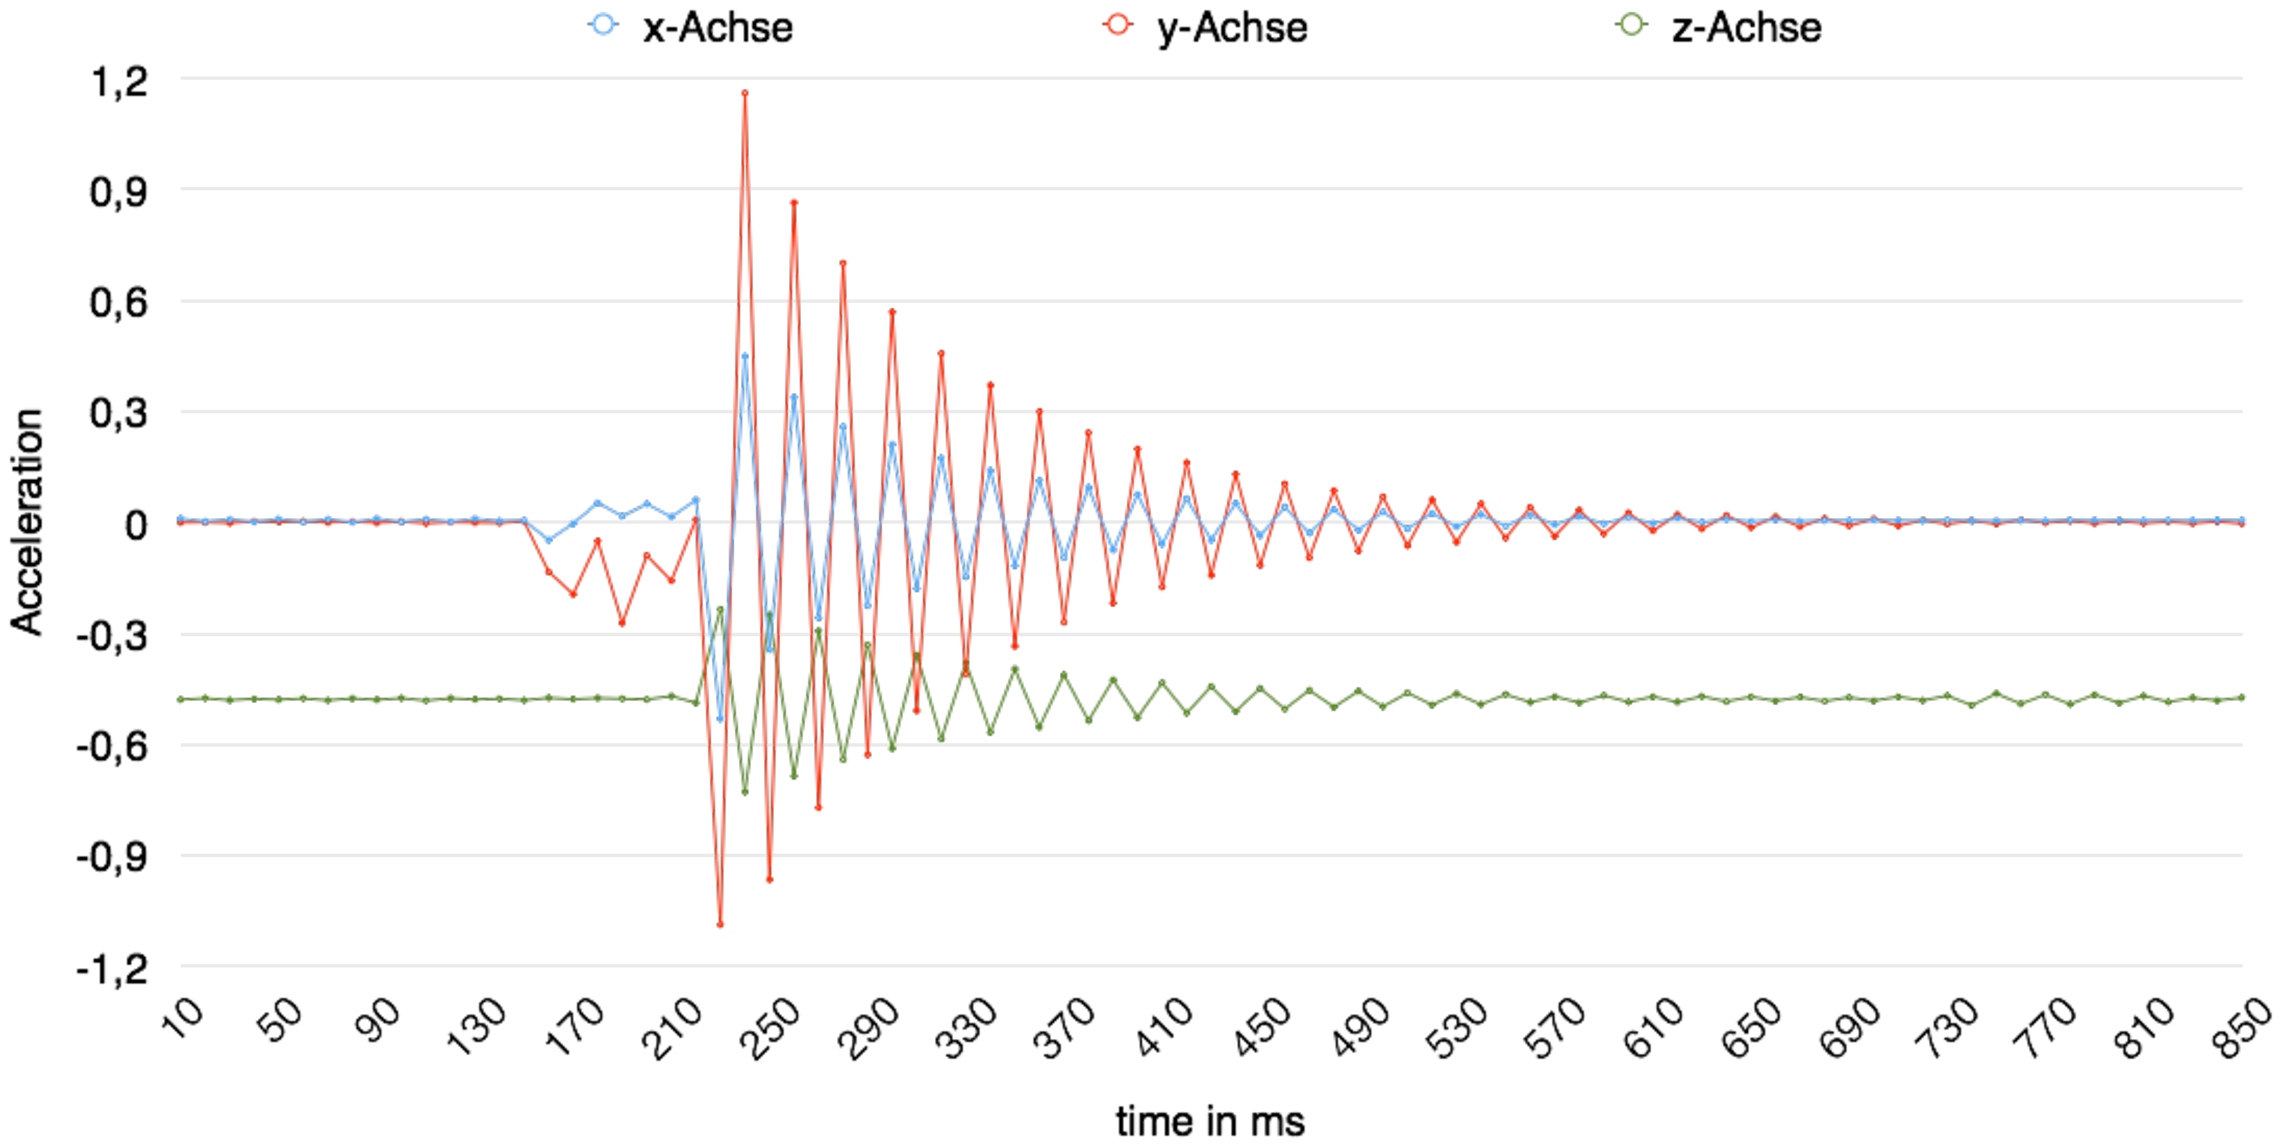
\includegraphics[width=1.0\textwidth]{kapitel4/acceleroLang.pdf}
    \caption{Bump-Muster Stirnseite an Stirnseite}
    \label{fig:stirnanstirn}
\end{figure}

\subsubsection{Längsseite an Längsseite}
Die Endgeräte werden aufrecht in den Händen der Anwender gehalten und werden an den Längsseiten zusammengestoßen.
\begin{figure}[H]
    \centering
    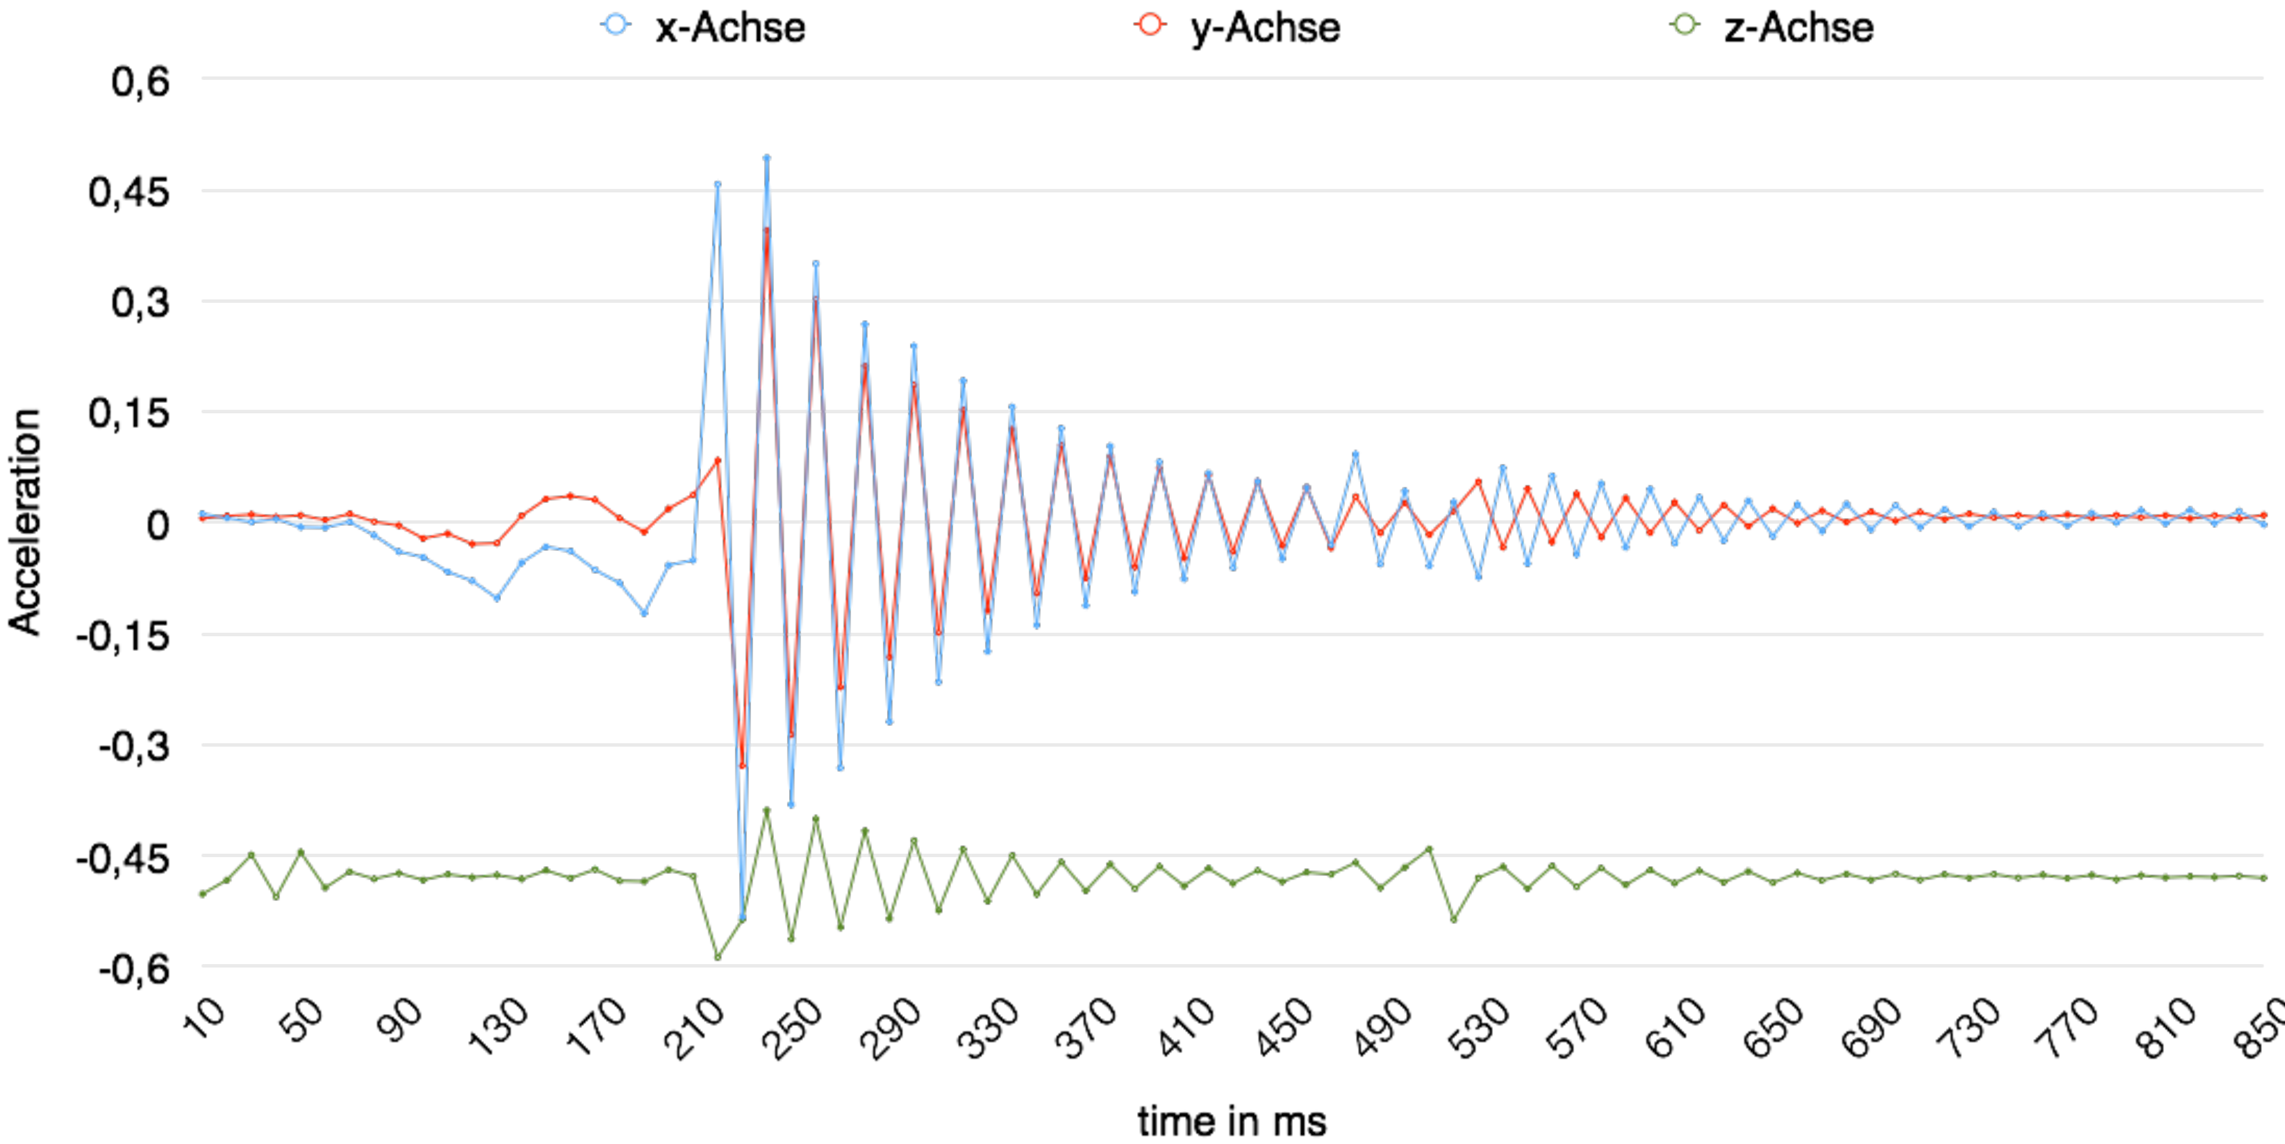
\includegraphics[width=1.0\textwidth]{kapitel4/acceleroBreit.pdf}
    \caption{Bump-Muster Längsseite an Längsseite}
    \label{fig:längsanlängs}
\end{figure}

\subsubsection{Ecke an Ecke}
Die Endgeräte werden aufrecht in den Händen der Anwender gehalten und werden an den oberen Ecken zusammengestoßen.
\begin{figure}[H]
    \centering
    \includegraphics[width=1.0\textwidth]{kapitel4/acceleroEcke.pdf}
    \caption{Bump-Muster Ecke an Ecke}
    \label{fig:eckeanecke}
\end{figure}

\subsubsection{Stirnseite aufstoßen}
Ein Endgerät wird vom Anwender aufrecht in der Hand gehalten und mit der oberen oder unteren Kante auf ein stationäres Gerät aufgestoßen.
\begin{figure}[H]
    \centering
    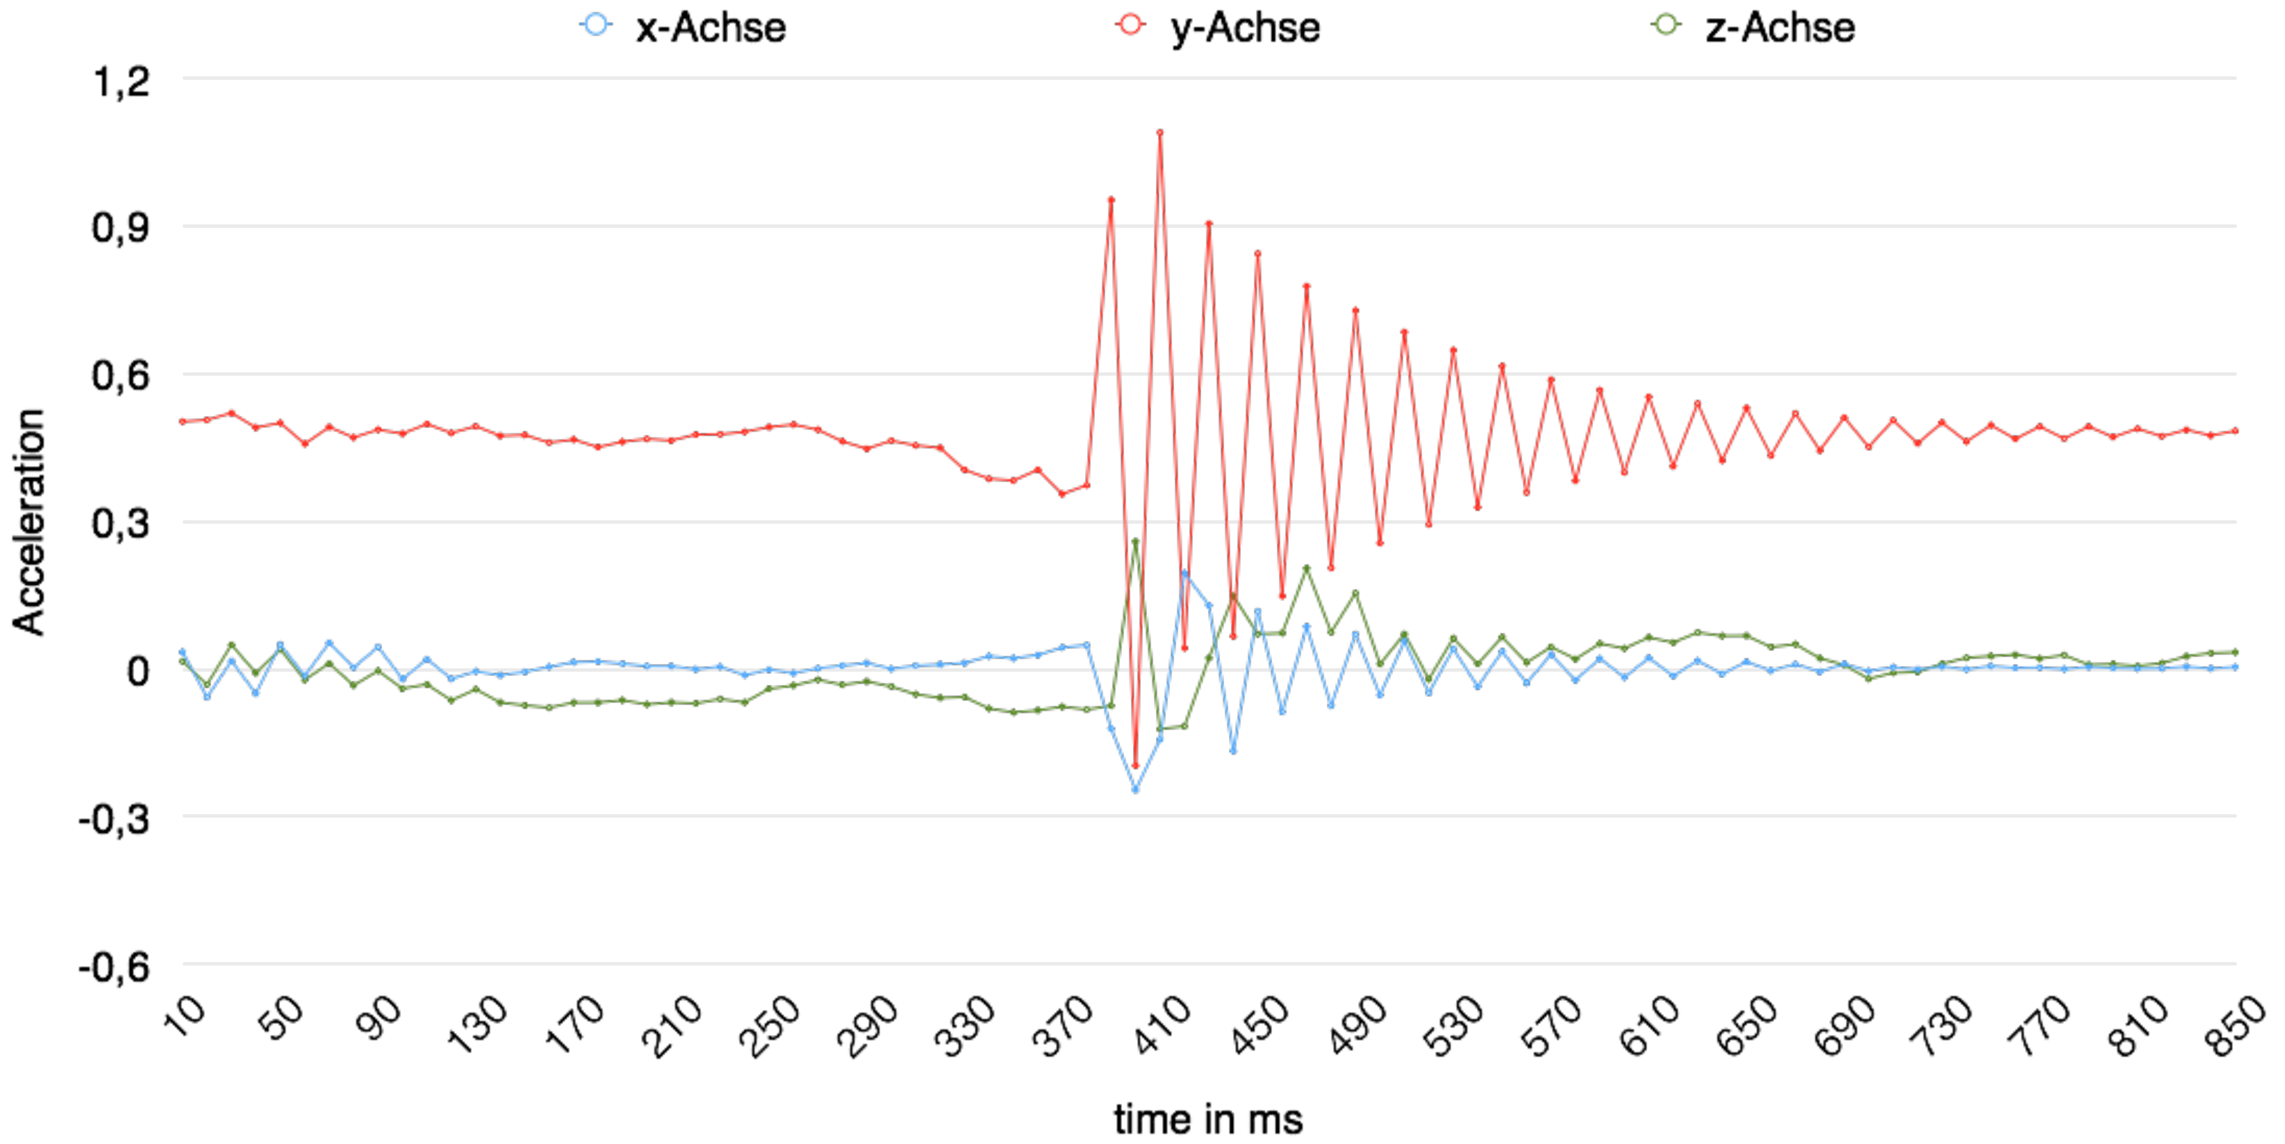
\includegraphics[width=1.0\textwidth]{kapitel4/acceleroOben.pdf}
    \caption{Bump-Muster Stirnseite aufstoßen}
    \label{fig:aufstossen}
\end{figure}

\subsubsection{Erkenntnisse aus den Versuchen}
Jede Bump-Variante generiert ein etwas anderes Muster. Es gibt jedoch Gemeinsamkeiten, die einen Bump typisieren und von anderen Bewegungen eines Benutzers unterscheiden. Die folgenden Charakteristiken können aus den Daten abgeleitet werden:
\begin{enumerate}
  \item Der Aufprall generiert initial eine hoch ausschlagende Flanke.
  \item Die nachfolgenden Daten sind alternierende Spitzen.
\end{enumerate}

\subsection{Algorithmus zur Mustererkennung}
Basierend auf den Beobachtungen aus den Versuchen, überprüft der Algorithmus die Daten des Beschleunigungssensors in zwei Schritten. Im ersten Schritt werden die Daten aller Achsen auf hoch ausschlagenden Flanken überprüft, welche einen Indikator für einen Bump darstellen. Dafür wird jeder Wert zwischengespeichert und mit dem Folgewert der Abstand (Siehe Abbildung \ref{fig:bump}) zwischen den Werten berechnet. 

\begin{figure}[H]
    \centering
    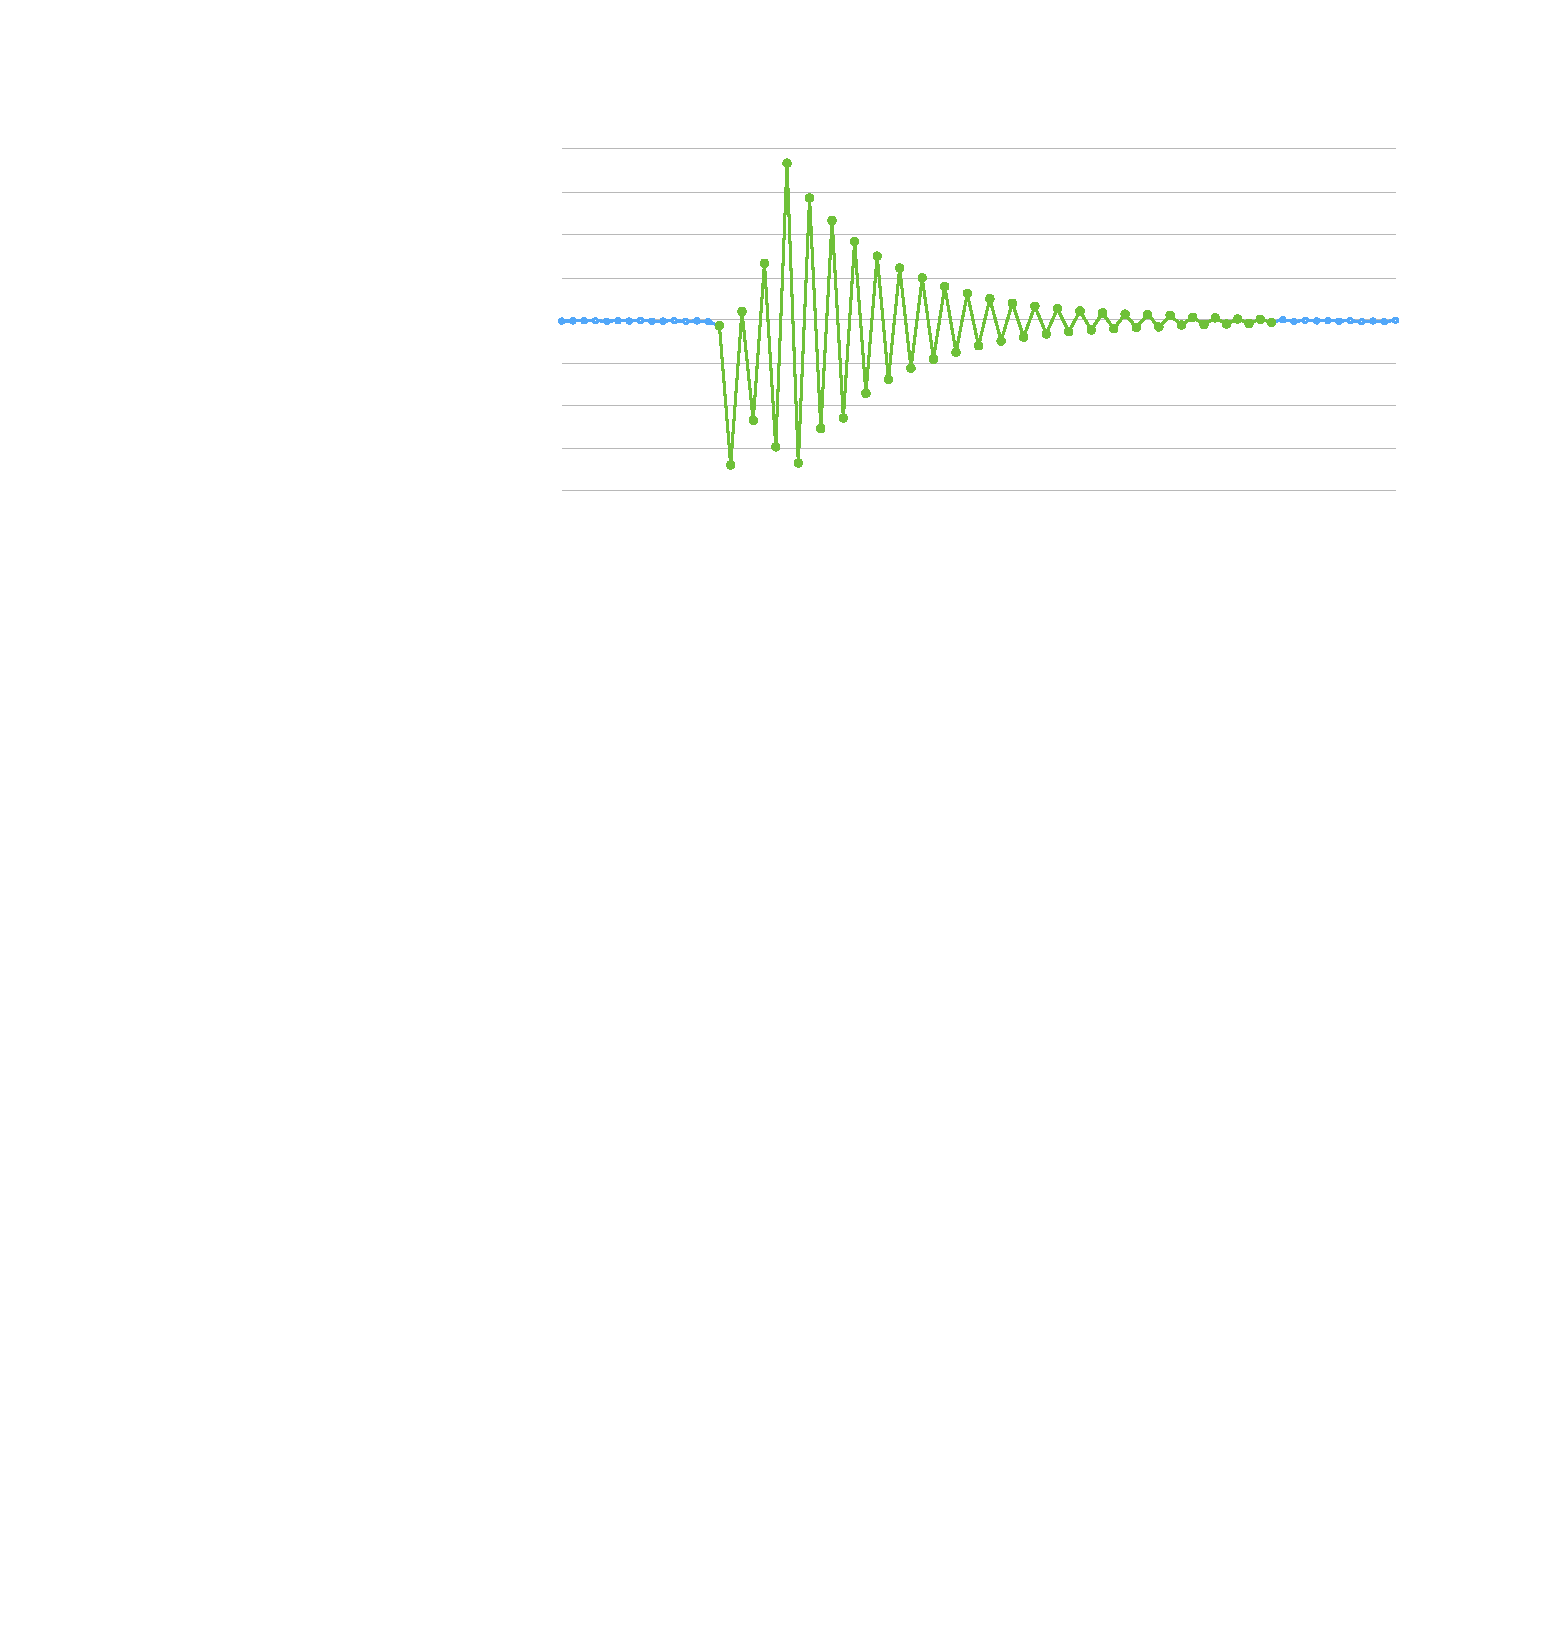
\includegraphics[width=1.0\textwidth]{kapitel4/acceleroBump.pdf}
    \caption{Algorithmische Erkennung eines Bumps}
    \label{fig:bump}
\end{figure}

Hat der Algorithmus initiale Flanken erkannt, wird im nächsten Schritt die durch die Kraft des Bumps beeinflussten Daten in einem Vektor für jede Achse aufgezeichnet. Um zu verifizieren, dass ein Bump stattgefunden hat, läuft anschließend eine Schleife über die Vektoren und zählt die Spitzen. Sind nur Spitzen im Vektor vorhanden, handelt es sich um einen Bump.

\newpage
\section{Konzepte zur Identifizierung von Bump-Partnern}
\label{sec:Ident}
Um Daten zwischen Bump-Partnergeräten, in einem lokalen Netzwerk oder über einen Server, auszutauschen müssen die Endgeräte, aus allen Teilnehmern eines Netzwerkes bzw. allen Clients die mit einem Server verbunden sind, ihren jeweiligen Partner identifizieren. Folgend werden zwei Verfahren vorgestellt mit denen diese Identifizierung erfolgen kann.

\subsection{Identifizierung über iBeacon Geräte-IDs}
Über die Major- und Minor-Werte kann mit iBeacon jedem Endgerät eine einzigartige ID zugeordnet werden mit der Endgeräte identifiziert werden können. Um diese ID zwischen Bump-Partnern auszutauschen, wird auf beiden Geräten iBeacon zum Zeitpunk des Bumps für kurze Zeit aktiviert. Gerade lange genug, damit die Endgeräte alle aktiven Beacons in ihrem Umfeld sehen können. Dadurch besitzt jedes Gerät eine Liste an Beacons die zu einen bestimmten Zeitpunkt an einem Bump, in ihrer Empfangsreichweite, beteiligt waren. Können die Endgeräte jeweils nur ein anderes Beacon sehen, haben Sie ihren Bump-Partner identifiziert. Ist mehr als ein Beacon sichtbar, fanden mehrere Bumps zeitgleich statt. In diesen Fällen können die Partner, über die Entfernung der Geräte zueinander, ermittelt werden. Bei den Geräten mit dem geringsten Abstand handelt es sich um die Bump-Partner. Die Erkennung der Partnergeräte über die Entfernung macht es erforderlich, dass zeitgleiche Bumps mindestens einige Zentimeter voneinander entfernt stattfinden. Dies stellt sicher, dass eine falsche Zuordnung durch ungenaue Abstandsmessungen vermieden wird.

\subsection{Identifizierung durch charakteristische Bump-Daten}
Ein Bump ist ein Ereignis, bei dem beteiligte Geräte verschiedene Daten erfassen können, die jeden Bump einzigartig charakterisieren. Eine Kombination aus Zeitpunkt und Standort bietet in den meisten Fällen eine ausreichende Datenbasis, um Bumps voneinander unterscheiden zu können. Der Zeitpunkt des Bumps kann mit einem Timestamp festgehalten werden. Bei der Nutzung von Timestamps muss jedoch beachtet werden, dass die Uhren der Geräte nicht synchron laufen. Um möglichst übereinstimmende Timestamps zu erhalten, sollte die Applikation deshalb die Systemuhr in bestimmten Zeitintervallen synchronisieren. Die Position der Endgeräte zum Zeitpunkt des Bumps kann über \ac{GPS} Koordinaten erfasst werden. Da sich Geräte bei einem Bump berühren, sollten im besten Falle die Koordinaten, die auf beiden Geräte ermittelt werden, übereinstimmen. Bei der Nutzung von \ac{GPS}muss aber beachtet werden, dass nicht immer eine genaue Positionsbestimmung garantiert ist. Trotz der etwaigen Abweichungen von sowohl Timestamp als auch \ac{GPS}, sollte eine Kombination dieser Daten in den meisten Fällen ausreichen, um Endgeräte zuverlässig einem Bump zuordnen zu können.

\subsection{Vergleich der Konzepte}
Der Vergleich von Timestamps und \acs{GPS}-Positionsdaten sollte in den meisten Fällen zuverlässige Zuordnung von Bump-Partnern ermöglichen. Jedoch erreicht das System seine Grenzen, wenn mehrere Bumps zum selben Zeitpunkt und am selben Standort stattfinden. Die potenzielle Ungenauigkeit von \ac{GPS} kann dazu führen, dass die jeweiligen Partnergeräte nicht zugeordnet werden können. Des weiteren kann gerade im Inneren von Gebäuden dieses System unter Umständen durch den verminderten Satellitenempfang gar nicht oder nur mit Einschränkungen genutzt werden. Zum Vergleich ist das System mit iBeacon und GeräteIDs in Innenräumen besser nutzbar als \ac{GPS} und ermöglicht, den Abstand zwischen Endgeräten genauer zu bestimmen. Die Identifizierung durch die Entfernungsmessung mit iBeacon besitzt aber auch ihre Grenzen. Finden zeitgleich Bumps in nur wenigen Zentimetern Entfernung zueinander statt, ist auch hier keine fehlerfreie Zuordnung garantiert. Im Vergleich ist iBeacon genauer als \acs{GPS} und sollte in den Fällen in denen der Abstand der Geräte entscheidend ist die besseren Ergebnisse erzielen.

\newpage
\section{Konzepte zum Datenaustausch}
\label{sec:Austausch}
Der Datenaustausch zwischen Endgeräten lässt sich über zwei verschiedene Ansätze realisieren. Zum einen können Daten direkt zwischen den Geräten über ein lokales Netzwerk getauscht werden und zum anderen über einen zentralen Server. Für beide Varianten werden folgend Konzepte vorgestellt, in denen sich Endgeräte identifizieren und Daten austauschen können.

\subsection{Datenaustausch über lokale Netzwerke}
Mit Hilfe von drahtlosen Netzwerktechnologien kann Datenaustausch zwischen Endgeräten entweder über ein WLAN-Infrastrukturnetzwerk oder durch die Bildung eines Ad-Hoc Netzwerkes realisiert werden. Unabhängig von der Topologie des Netzwerkes läuft die Kommunikation zwischen den Netzwerkteilnehmern über Netzwerkdienste. Entscheidend ist dabei, dass sich die an einem Bump-Event beteiligten Geräte im Computernetzwerk gegenseitig identifizieren können. Folgend wird einleitend beschrieben wie die beiden in \ref{sec:Ident} beschriebenen Konzepte in lokalen Netzwerken angewendet werden. Anschließend werden für beide Möglichkeiten der genaue Ablauf des Verbindungsaufbaus zwischen den Geräten beschrieben.

\subsubsection{Geräteidentifizierung in lokalen Netzwerken}
Es werden zwei Maßnahmen ergriffen, mit denen sichergestellt werden soll, dass sich die an einem Bump beteiligten Geräte zuverlässig identifizieren. Im ersten Schritt wird dazu die Anzahl an Netzwerkteilnehmern, die den selben Netzwerkdienst zeitgleich verwenden, verringert. Dazu wird der Netzwerkdienst, der von der Bump-Applikation angeboten wird, erst gestartet, nachdem das Bump-Event stattgefunden hat und wieder gestoppt, sobald zwischen den Bump-Partnern eine Verbindung aufgebaut wurde. Dadurch ist der Netzwerkdienst nur für kurze Zeit bei jenen Endgeräten aktiv, die zum gleichen Zeitpunkt einen Bump durchgeführt haben. Der Zeitraum, in dem der Netzwerkdienst von den Bump-Partner angeboten und gesucht wird, ist sehr kurz, in den meisten Fällen werden deswegen immer nur Bump-Partner gleichzeitig den selben Netzwerkdienst nutzen, wodurch eine weitere Identifizierung gar nicht nötig wäre (Siehe Abbildung \ref{fig:dienste} a).

\begin{figure}[H]
    \centering
    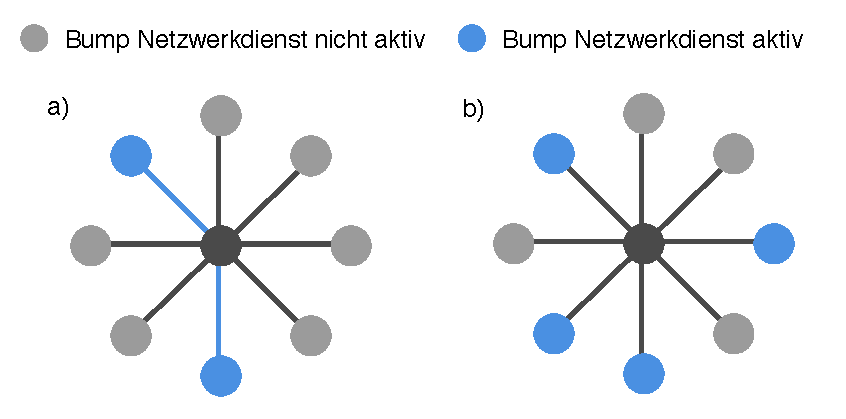
\includegraphics[width=\linewidth]{kapitel4/netzwerkdienste.pdf}
    \caption{Netzwerkdienste in einem Infrasturkturnetzwerk}
    \label{fig:dienste}
\end{figure}

Da jedoch nicht sichergestellt werden kann, dass in der Zeitspanne in der Bump-Partner den Netzwerkdienst nutzen, kein weiterer Bump auftritt und dadurch mehr als zwei Engeräte den Netzwerkdienst nutzen (Siehe Abbildung \ref{fig:dienste} b), wird zusätzlich noch eine der in Abschnitt \ref{sec:Ident} beschriebenen Methode benötigt, mit der sich Bump-Partner im Netzwerk identifizieren können (Siehe Abbildung \ref{fig:diensteIdent}).

\begin{figure}[H]
    \centering
    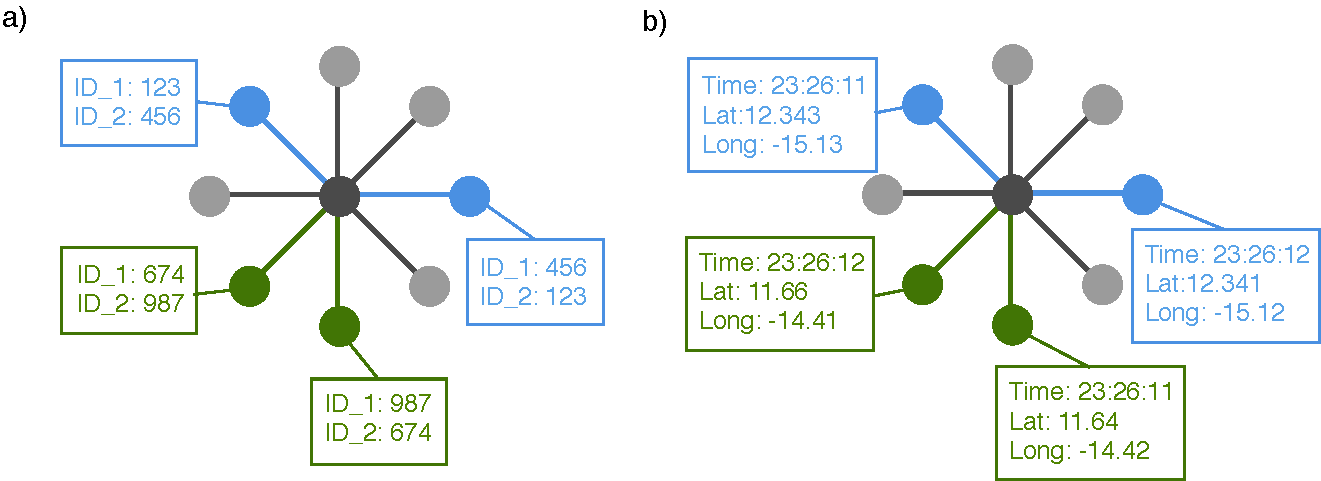
\includegraphics[width=\linewidth]{kapitel4/netzwerkdiensteIdent.pdf}
    \caption{Identifizierung von Netzwerkteilnehmern}
    \label{fig:diensteIdent}
\end{figure}

\newpage
\subsubsection{Ablauf mit iBeacon Geräte-IDs}
Wird auf einem Gerät ein Bump registriert, ist der erste Schritt die Generierung von Zufallszahlen für den Major- und Minor-Wert von iBeacon. Diese Zahlen bilden eine eindeutige ID, mit der sich jedes Gerät im Netzwerk identifizieren kann. Anschließend wird iBeacon aktiviert, die Geräte können sich gegenseitig sehen, GeräteIDs lesen und die Distanz zu allen sichtbaren Beacons erfassen. Ist mehr als ein Beacon sichtbar, wird jenes ermittelt, welches die geringste Distanz zum suchenden Gerät aufweist. Die GeräteID dieses Geräts wird lokal gespeichert und iBeacon wird deaktiviert. Anschließend startet die DiscoveryPhase des Multipeer-Connectivity-Frameworks. In dieser Phase agiert das Gerät, dessen Minor Wert den kleineren Zahlenwert aufweist, als Advertiser und bietet einen Netzwerkdienst an. Die discoveryInfo dieses Dienstes enthält die durch Major und Minor gebildete GeräteID des Advertisers. Das Gerät mit dem höheren Zahlenwert ist der Browser und sucht den Dienst des Advertisers. Diese Aufgabenverteilung verhindert, dass Probleme beim Verbindungsaufbau auftreten, sollten sich die Geräte gleichzeitig zu einer Session einladen.
Findet der Browser diesen Dienst, kann er die GeräteID des Advertisers mit der GeräteID vergleichen, die das zu Beginn ermittelte Beacon aufweist. Stimmen die IDs überein, handelt es sich bei dem Advertiser um den Bump-Partner und der Browser kann eine Session erstellen und eine Einladung zu dieser an den Advertiser schicken. Mit dieser Einladung wird in der contextData wiederum die GeräteID des Browsers mitgeschickt. Damit kann der Advertiser überprüfen, ob er auch wirklich von seinem Partner eingeladen wird und nicht von jemand anderem. Haben die Geräte eine Verbindung aufgebaut, können Sie über die Methoden des Frameworks die gewünschten Daten austauschen, und anschließend die Session verlassen. 

Der beschriebene Ablauf kann auch noch einmal im folgenden UML Diagramm nachvollzogen werden.

\begin{figure}[H]
    \centering
    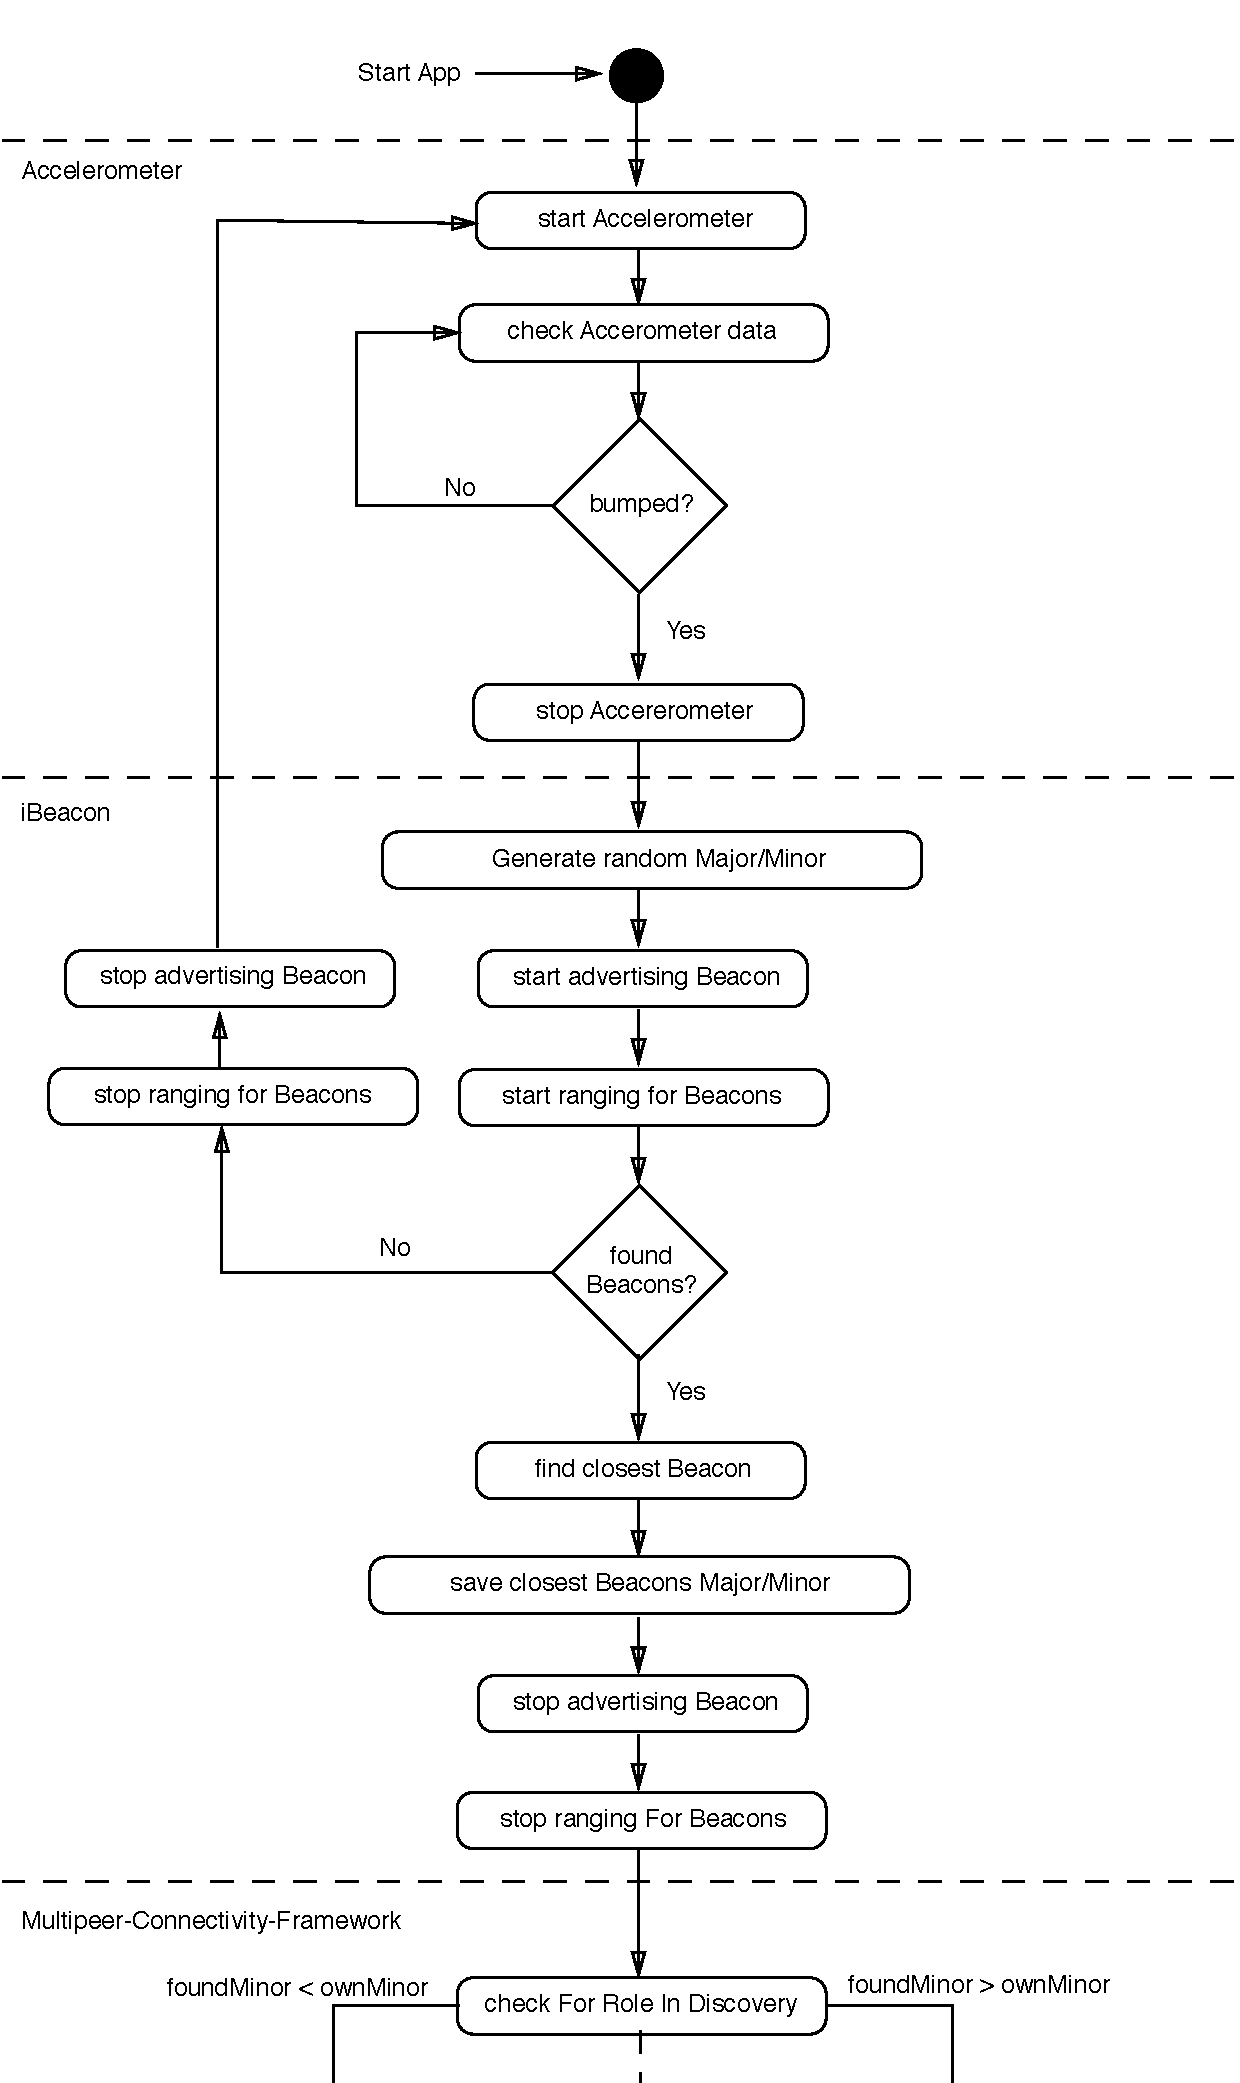
\includegraphics[width=\linewidth]{kapitel4/umlkurz1.pdf}
    \label{umlBecon1}
    \caption{System mit iBeacon UML Diagramm}
\end{figure}
\begin{figure}[H]
    \centering
    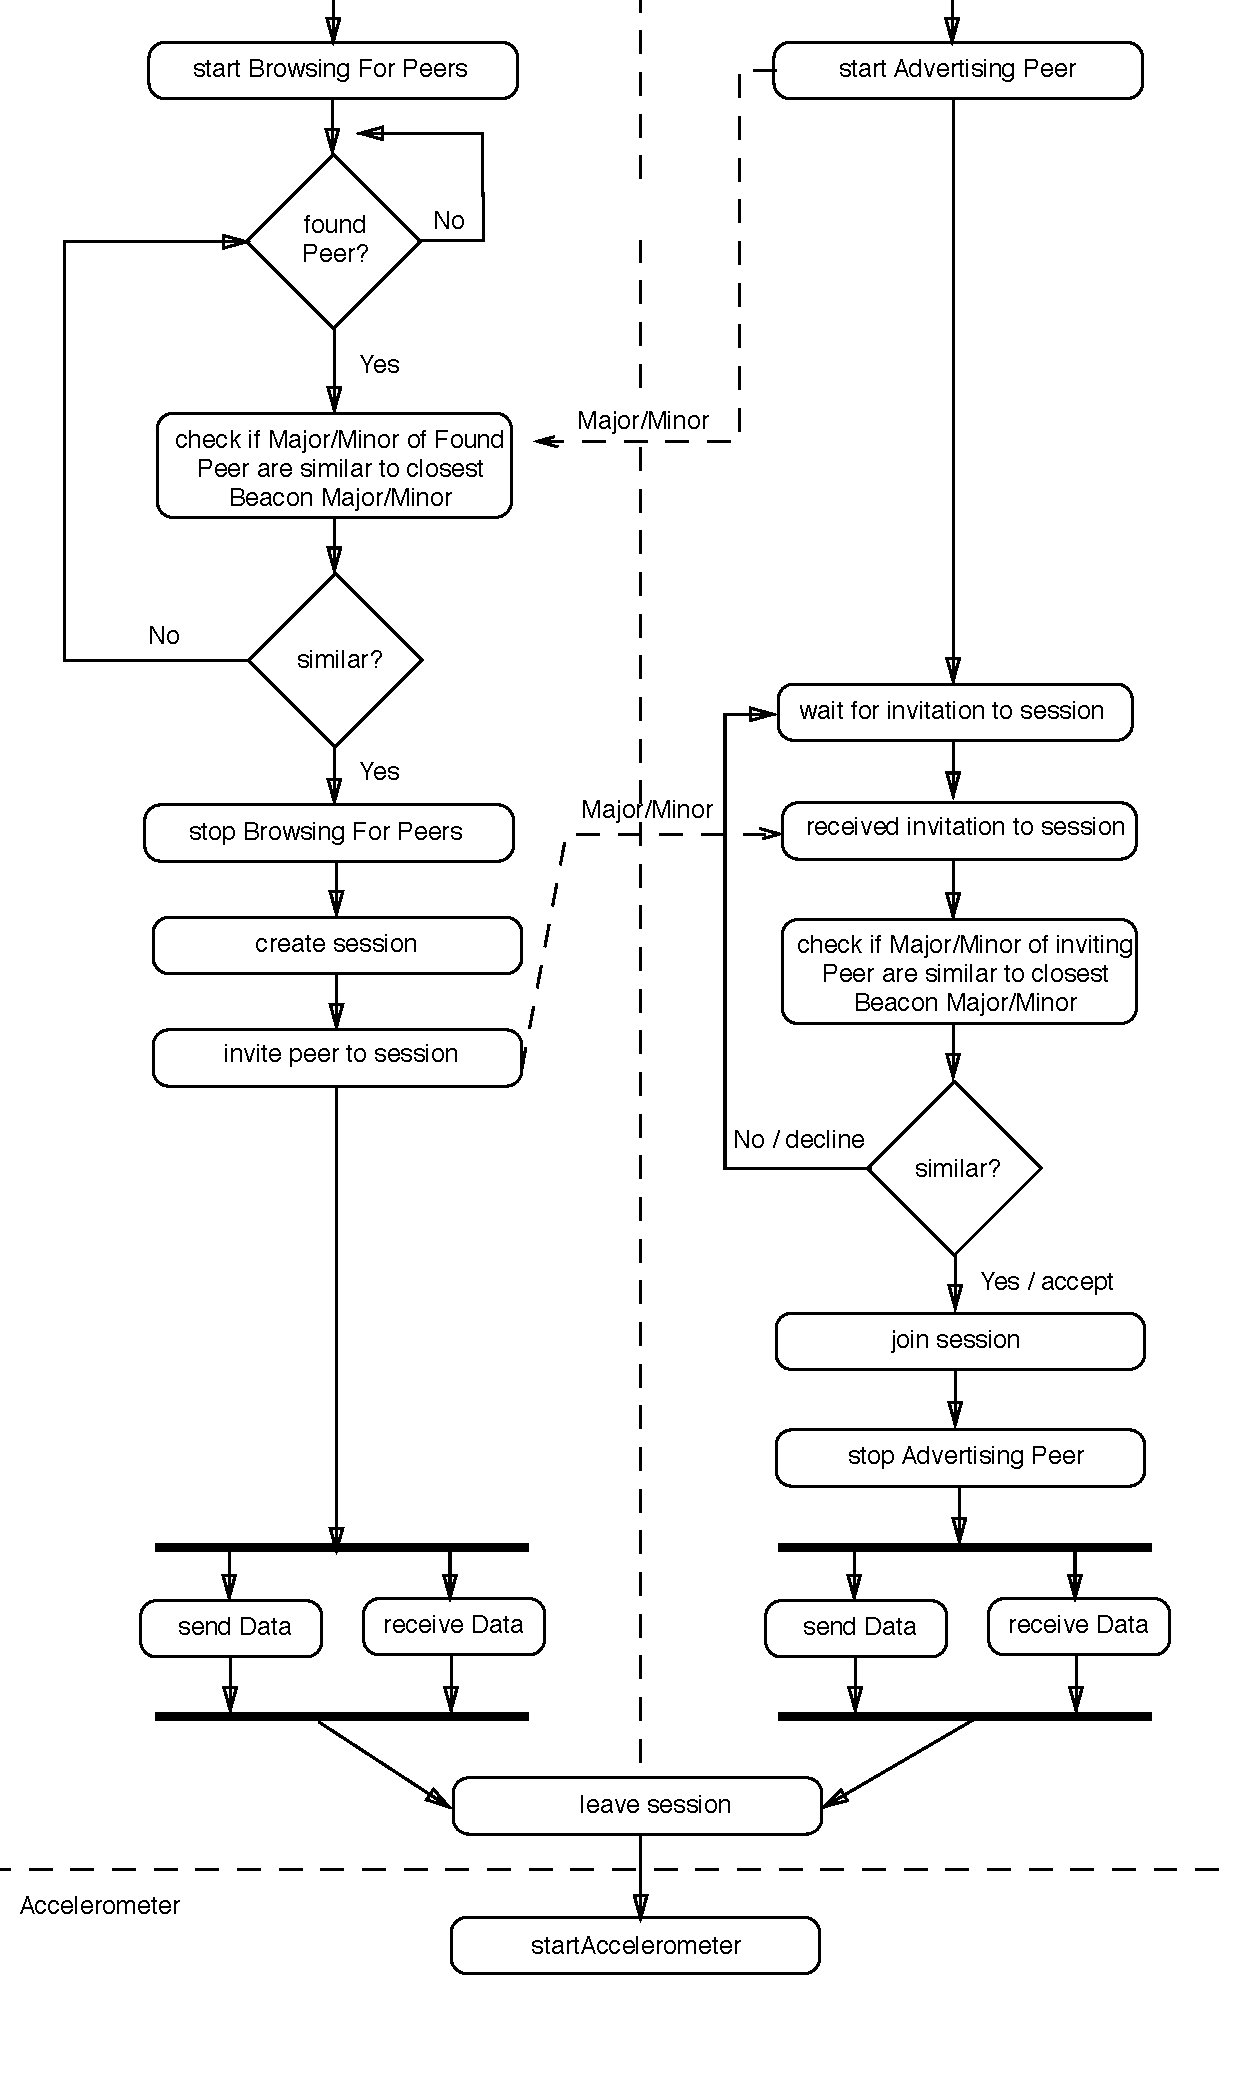
\includegraphics[width=\linewidth]{kapitel4/umlkurz2.pdf}
    \label{umlBecon2}
    \caption{System mit iBeacon UML Diagramm}
\end{figure}

\subsubsection{Ablauf mit Timestamp und GPS}
Mit Timestamp und \ac{GPS} läuft der Verbindungsaufbau etwas anders ab, als mit iBeacon. Zuerst werden die \ac{GPS} Daten der Endgeräte erfasst und lokal gespeichert. Im nächsten Schritt eröffnen beide Endgeräte einen Browser- und Advertiser-Dienst mit einem gemeinsamen Bezeichner. Die zuvor gespeicherten \ac{GPS} Daten werden bei beiden Geräten in der discoveryInfo zusammen mit einer generierten Zufallszahl untergebracht. Beide Geräte können nun auf Timestamp und \ac{GPS} Daten der gefundenen Geräte zugreifen und Timestamp und \ac{GPS} Daten mit den eigenen abgleichen. Stimmen die gefundenen Daten mit den eigenen überein, wurde identifiziert welches Gerät zu einer Session eingeladen werden muss. Wer diese Session erstellt und den Partner zu dieser einlädt, wird über die generierte Zufallszahl die ebenfalls in der discoveryInfo gespeichert wird, ausgehandelt. Nachdem die Session zustande gekommen ist, werden die Netzwerkdienste deaktiviert und der Datenaustausch kann erfolgen.

Der beschriebene Ablauf ist im folgenden UML Diagramm noch einmal dargestellt.

\begin{figure}[H]
    \centering
    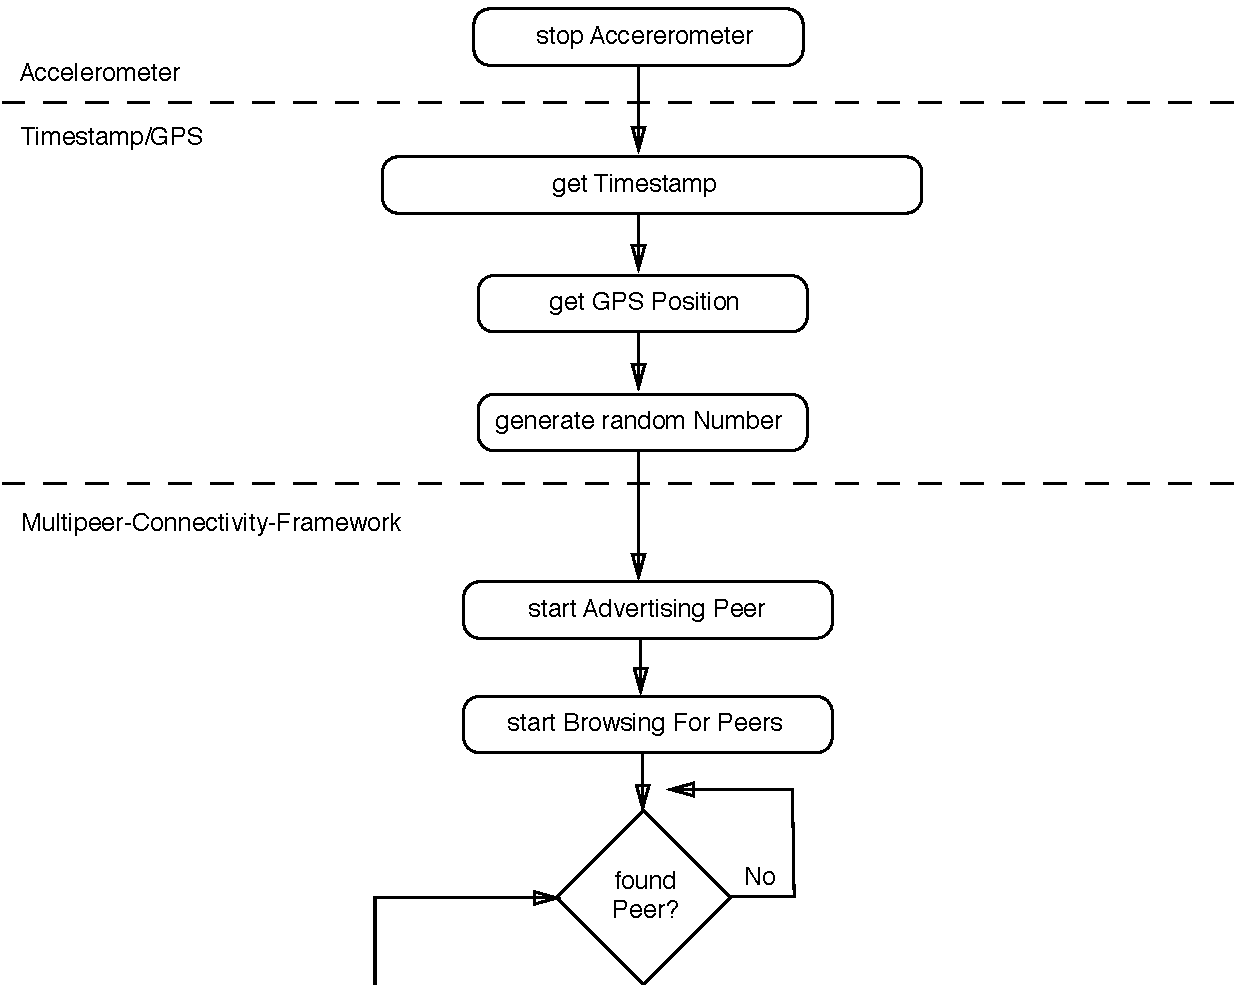
\includegraphics[width=\linewidth]{kapitel4/umlGPS.pdf}
    \label{umlGPS1}
    \caption{System mit Timestamp und GPS UML Diagramm}
\end{figure}
\begin{figure}[H]
    \centering
    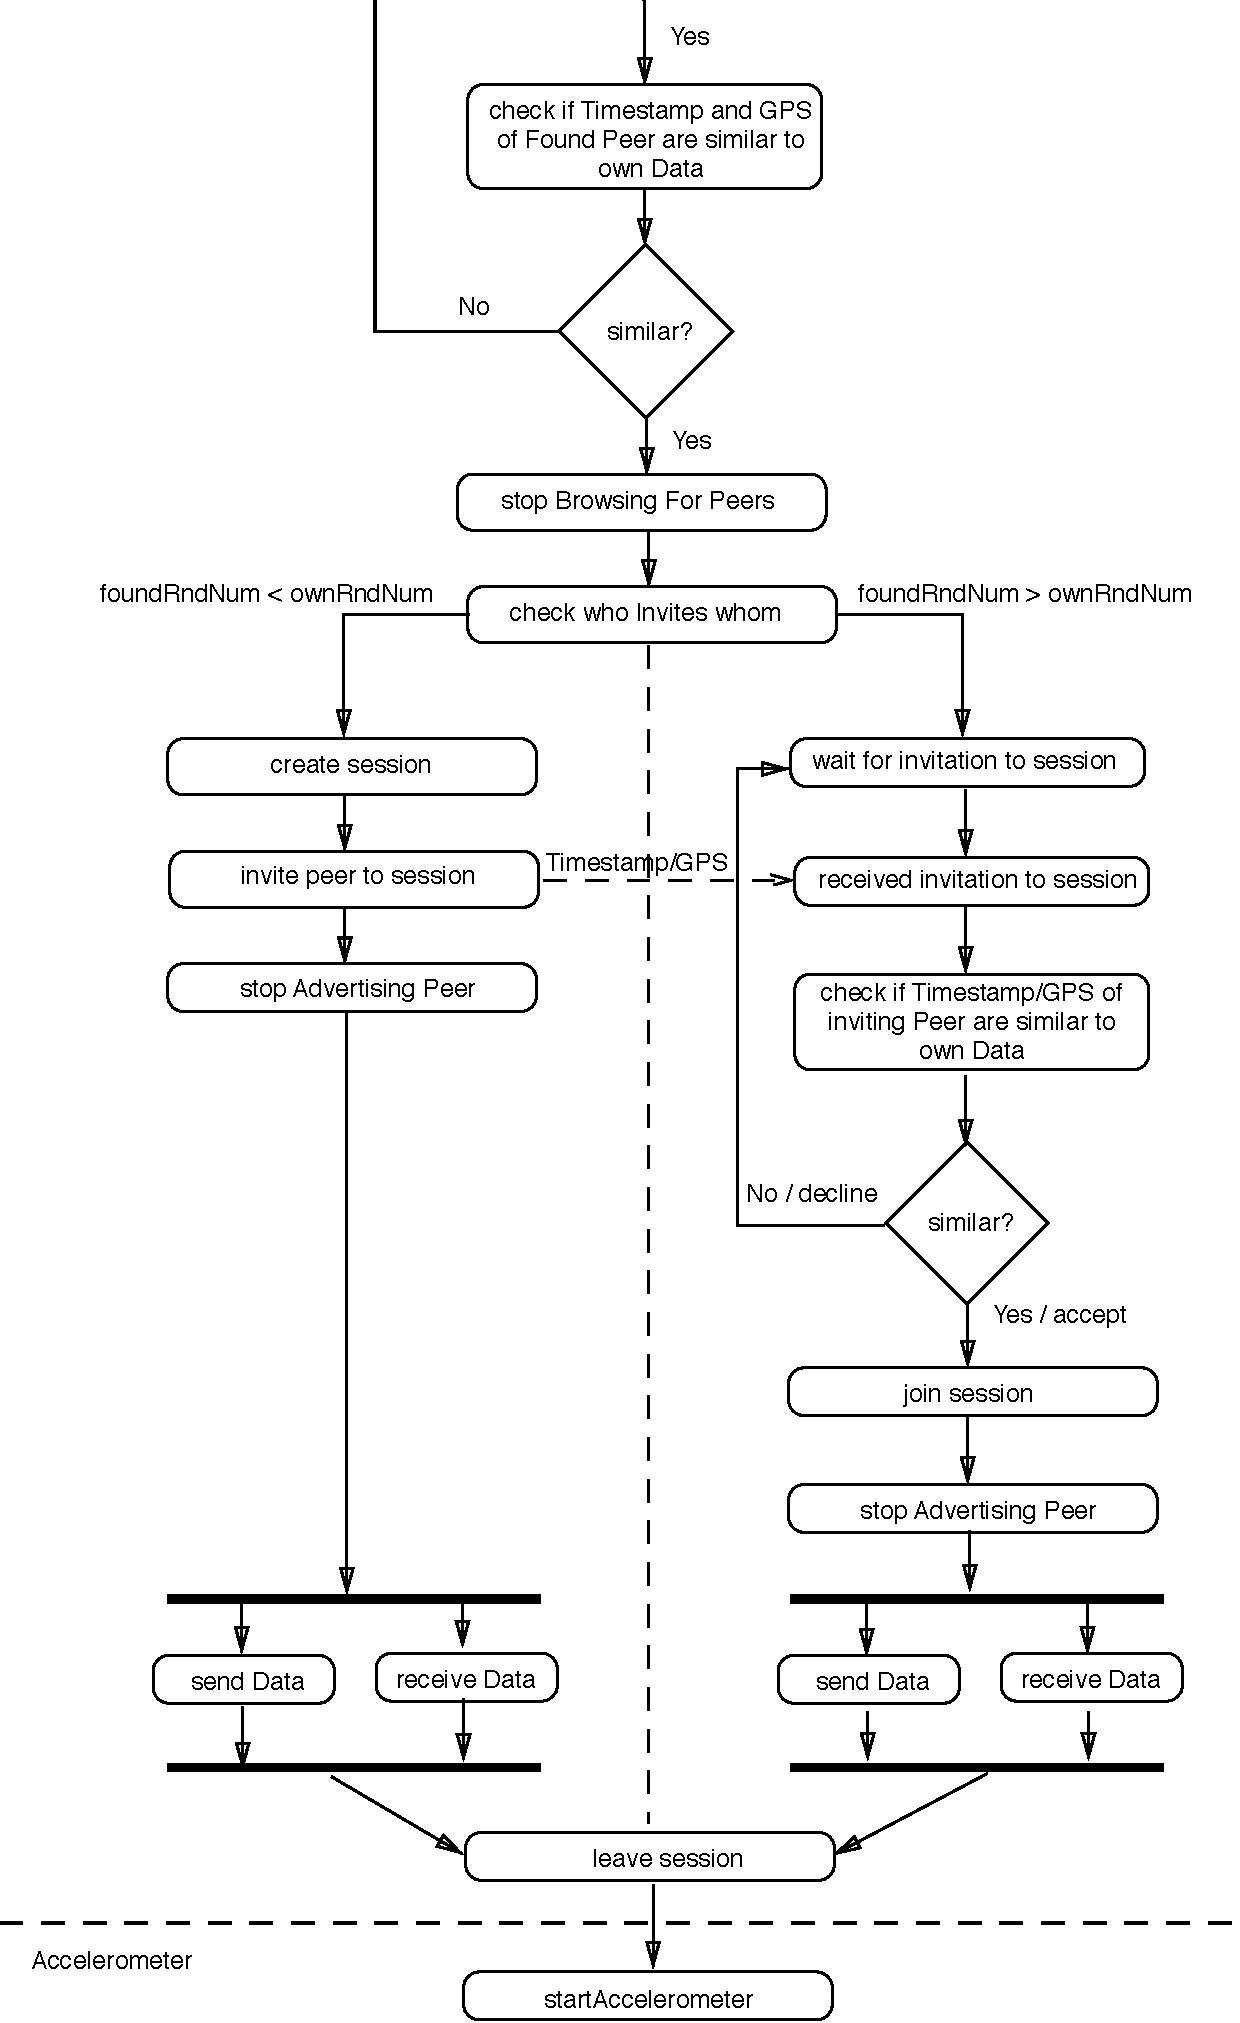
\includegraphics[width=\linewidth]{kapitel4/umlGPS2.pdf}
    \label{umlGPS2}
    \caption{System mit Timestamp und GPS UML Diagramm}
\end{figure}

\subsection{Datenaustausch über Webserver}
\label{sec:AustauschWebserver}

Die Kommunikation der Endgeräte über Webserver ist eine alternative Möglichkeit den Datenaustausch zwischen den Endgeräten zu implementieren. Im folgend beschriebenen System werden zwei Server genutzt, die nach verschiedenen Aufgaben aufgeteilt sind. Einer der Server, im folgenden als Fileserver bezeichnet, dient als Austausch Plattform für die von den Anwendern ausgewählten Daten. Diese werden von den Endgeräten auf den Server hochgeladen und sind dort anschließend unter einer bestimmten \acs{URL} erreichbar. Für die Übermittlung der \acs{URL} von Sender zu Empfänger ist der zweite Server, im folgenden als Messaging-Server bezeichnet, zuständig. Mit diesem Server verbinden sich die Bump-Partner über WebSockets und sind damit Teil eines Nachrichtensystems, mit dem der Server Nachrichten von allen verbundenen Endgeräten empfangen, aber auch senden kann. Damit der Matchmaking-Server die Nachrichten an die richtigen Geräte weiterleiten kann, müssen diese wie auch in lokalen Netzwerken identifiziert werden. Wie die Kommunikation mit den einzelnen Servern genau abläuft, wird folgend erklärt.

\subsubsection{Ablauf der Kommunikation}
Verbinden sich Clients über WebSockets mit einem Server, wird jeder Socket mit einer eigenen SocketId erstellt. Über diese SocketID kann der Server einem bestimmten Client gezielt Nachrichten zuschicken. Da die Bump-Partnergeräte die SocketID des anderen nicht kennen, muss die SocketID auf dem Server mit zusätzlichen Informationen verknüpft werden, durch die der Server Bump-Partner einander zuordnen kann. Aus diesem Grund senden die Clients beim verbinden zum Server ihre GeräteIDs oder Timestamp und \acs{GPS} an den Server. Dieser erstellt anschließend ein User Objekt, speichert in diesem die SocketID zusammen mit den Identifikationsinformationen und fügt es einer Liste mit allen verbundenen Clients hinzu. Möchten Endgeräte ihren Partnern eine Nachricht schicken, müssen sie z.B. nur die GeräteID ihrer Partners mitsenden und der Server kann anhand dieser ID die SocketID über das User Objekt ermitteln und die Nachricht weiterleiten. Sobald sich beide Partnergeräte verbunden haben, informiert der Server die jeweiligen Clients darüber. Daraufhin können die Endgeräte die vom Anwender ausgewählten Daten auf den Fileserver hochladen, der ihnen, sobald der upload abgeschlossen ist, eine \acs{URL} zurückliefert, an der die Daten gespeichert sind. Diese \acs{URL} kann anschließend über den Messaging-Server an das Partnergerät übermittelt werden, das darauf den Download vom Fileserver starten kann. Sobald die Endgeräte jeweils ihre Downloads abgeschlossen haben, können Sie sich vom Messaging-Server abmelden und der Datenaustausch ist abgeschlossen. Im folgenden ist ein kleiner Codeausschnitt zu finden, in dem exemplarisch einige Funktionen zur WebSocket Kommunikation für den beschriebenen Ablauf dargestellt sind. Außerdem kann der beschriebene Ablauf noch einmal im Sequenzdiagramm (\ref{fig:sequenz}) nachvollzogen werden.

\lstinputlisting[firstline=1,language=Java]{\srcloc/source.java}

\begin{figure}[H]
    \centering
    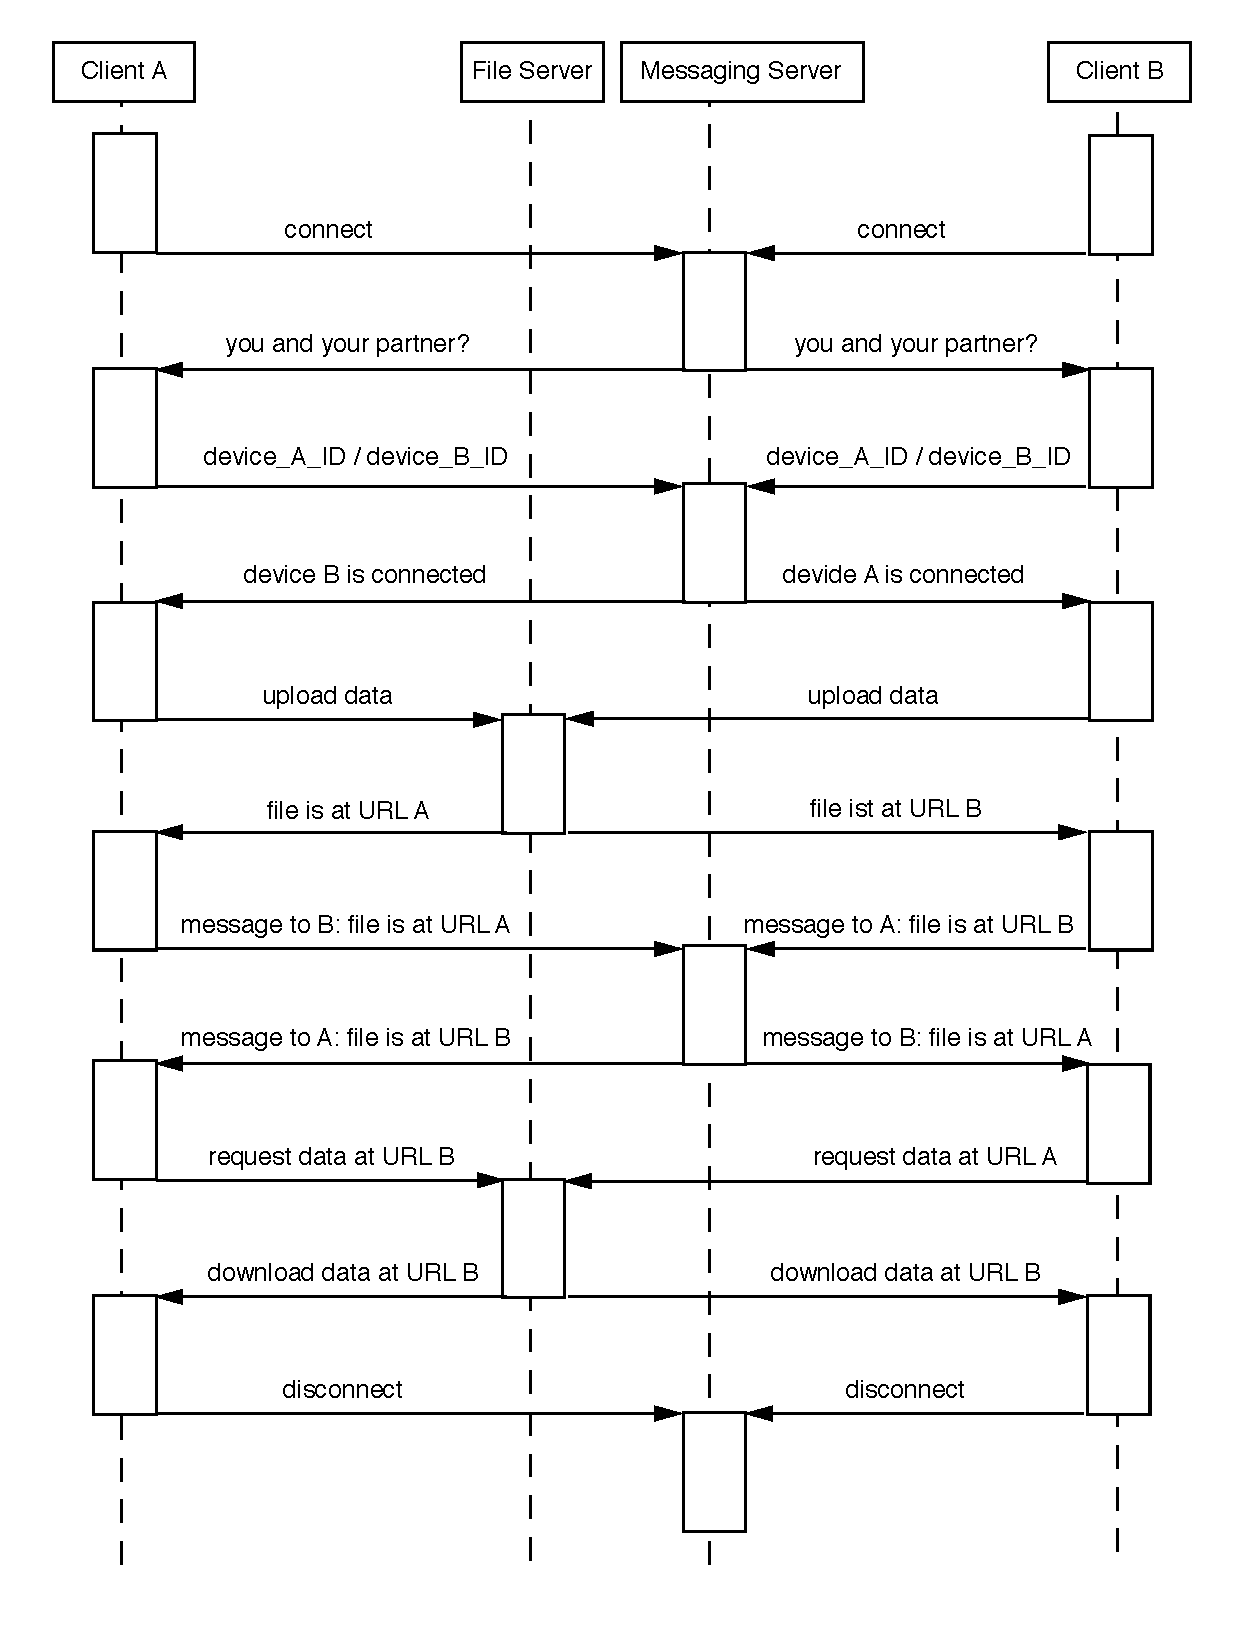
\includegraphics[width=\linewidth]{kapitel4/umlServer.pdf}
    \caption{Sequenzdiagramm Datenaustausch über Webserver}
    \label{fig:sequenz}
\end{figure}

\newpage
\subsection{Vergleich der Konzepte}
\label{sec:Systemvergleich}
Direkte Kommunikation bietet den Vorteil, ohne zusätzliche Server Infrastruktur zu operieren und es wird, falls der Server nur über das Internet erreichbar ist, auch keine Internetverbindung benötigt. Nachteilig ist jedoch der höhere Implementierungsaufwand, um für jede Plattform ein System anzubieten. Die von den Plattformen genutzten Technologien und Frameworks sind teilweise nicht kompatibel, was es erforderlich macht, für jede Plattform Einzellösungen zu implementieren. Wird dagegen eine Serverarchitektur gewählt, ist der Implementierungsaufwand wesentlich geringer, da die meiste Implementierung nur einmal für den Server erfolgen muss. Nachteilig ist der erforderliche Zugang zu entweder einem lokalen \ac{WLAN} oder zu mobilem Internet. Weiterhin handelt es sich bei einem Server um einen Single-Point-Of-Failure. Fällt der Server aus, funktioniert das komplette System nicht mehr. Hier bieten lokale Lösungen einen klaren Vorteil, da diese ausfallsicher sind. Weiterhin ist der Betrieb eines Servers auch mit Kosten verbunden die in einem lokalen System nicht anfallen. % Externe Datei einbinden
\chapter{Demonstrator Applikation}
\label{Kap5}
\label{chap:Kap5}
Als praktischer Teil dieser Arbeit wurde das Netzwerk basierte System implementiert. Mit der Applikation können zwei Anwender auf Endgeräten gespeicherte Fotos auswählen und durch einen Bump übertragen.

Die Implementierung wurde auf der iOS Plattform in der Programmiersprache Swift durchgeführt und ist als Git Repository erreichbar unter:

\url{https://github.com/informatik-mannheim/thesis-bump-to-transfer/tree/master/sources/Bumper}

Für das User-Interface der Applikation wurde ein Wireframe erstellt, das als PDF aufzufinden ist unter:

\url{https://github.com/informatik-mannheim/thesis-bump-to-transfer/blob/master/sources/Wireframe.pdf}

Folgend wird das Wireframe in Auszügen dargestellt um einen Einstieg in die Nutzung der Applikation zu bieten. Auf den Screenshots ist sichtbar welche Interaktionsmöglichkeiten dem Anwender, vor und nach der Durchführung der Interaktion, geboten werden. Von besonderem Interesse ist dabei zum einen wie der Anwender gespeicherten Inhalte durchsuchen und für den Versand auswählen kann und zum anderen wie empfangene Daten angezeigt und gespeichert werden können.

\subsubsection{}
\begin{figure}[H]
  \centering
  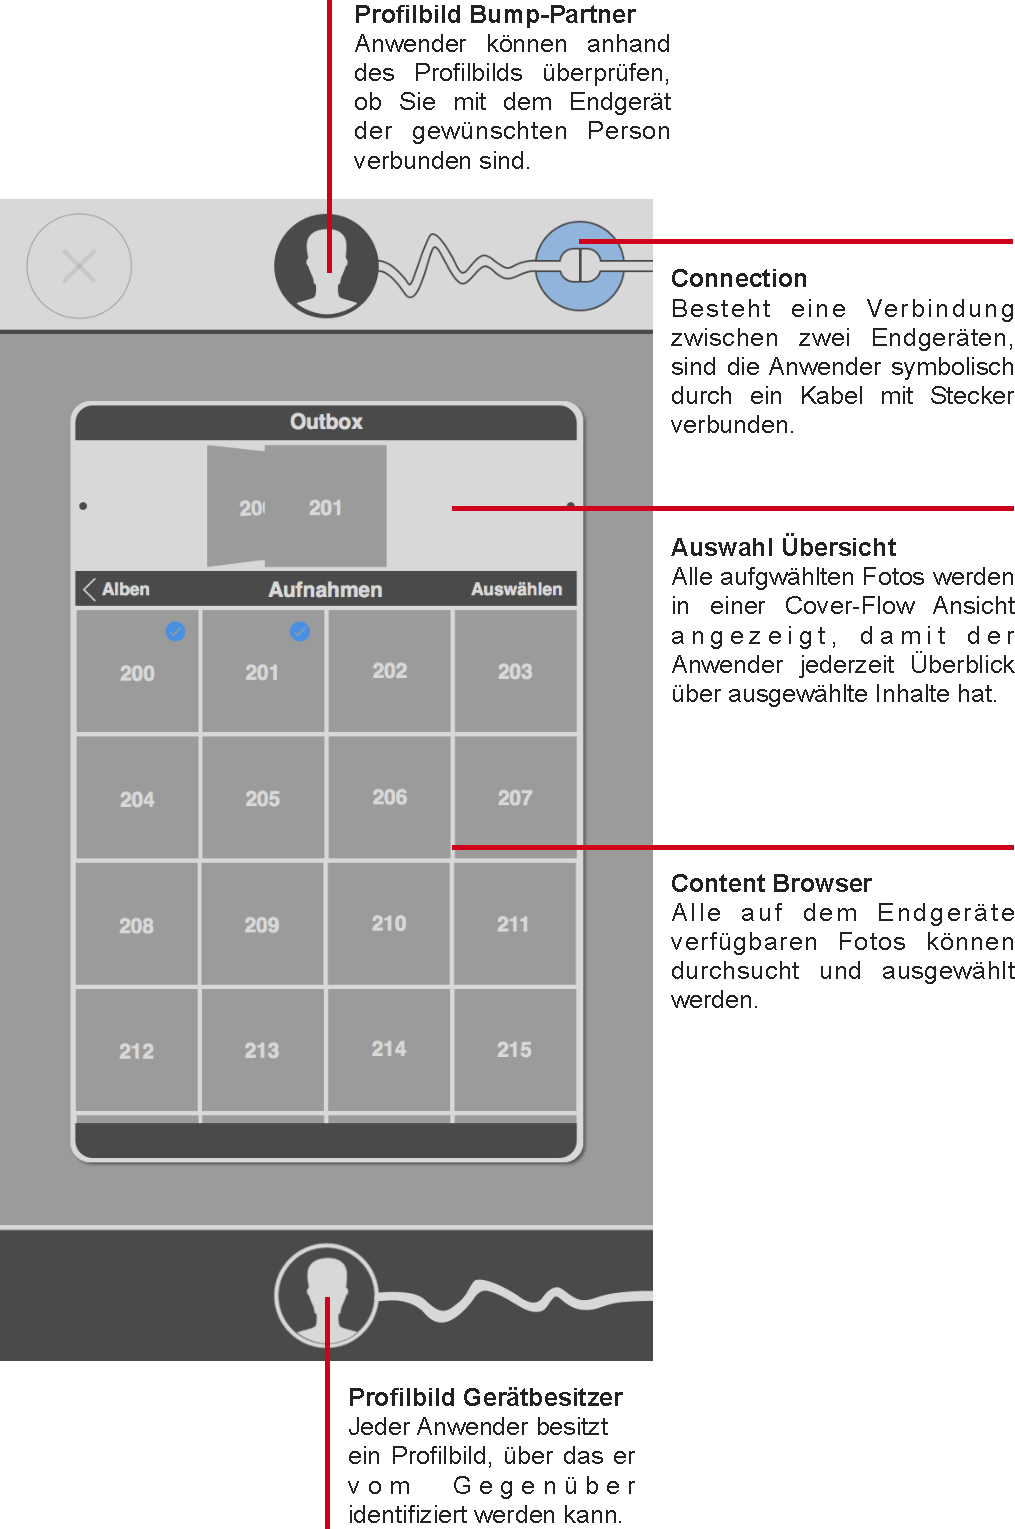
\includegraphics[width=\linewidth]{kapitel5/wireframe1.pdf}
\end{figure}

\subsubsection{}
\begin{figure}[H]
  \centering
  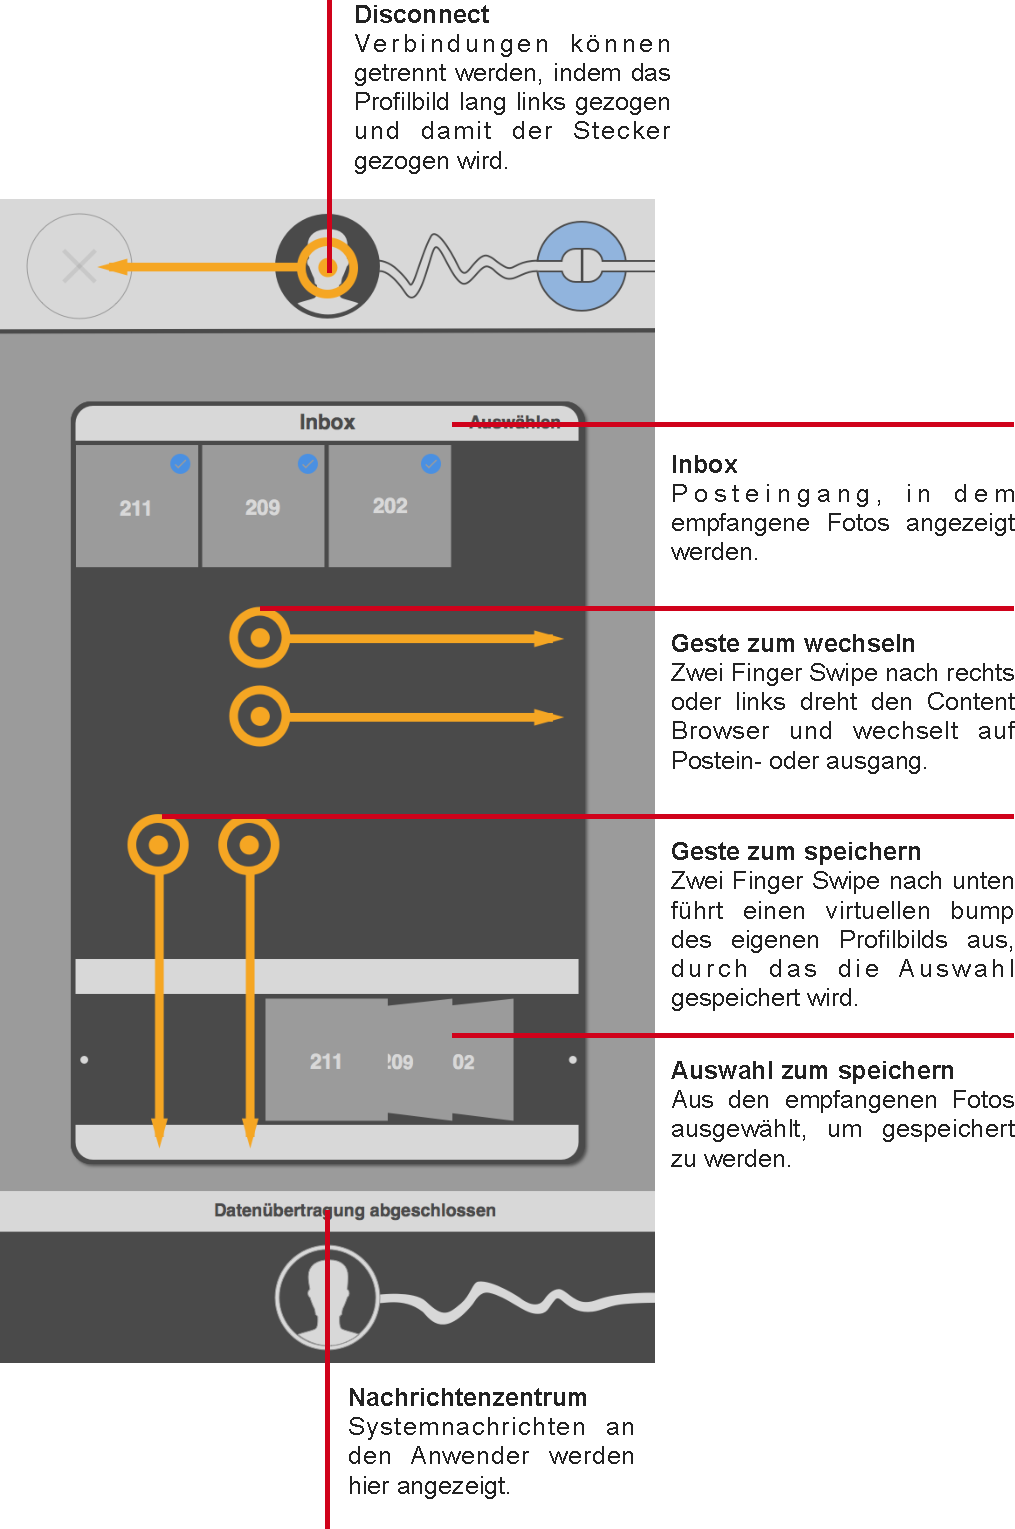
\includegraphics[width=\linewidth]{kapitel5/wireframe2.pdf}
\end{figure} % Externe Datei einbinden
\chapter{Zusammenfassung und Ausblick}
\label{Kap6}
\label{chap:Kap6}

Das zu Beginn dieser Arbeit formulierte Ziel wurde durch die folgenden Teilschritte erreicht: Zu Beginn wurde beschrieben, in welchen Varianten die Bump-Geste durchgeführt werden kann und welche Kategorien von Endgeräten für die Geste geeignet sind. Es wurden anschließend Technologien identifiziert, die eine Umsetzung der Geste auf mobilen Endgeräten ermöglicht. Für die Erkennung von Bumps wurde untersucht welche Daten von einem Beschleunigungssensor durch einen Bump erzeugt werden. Basierend auf diesen Erkenntnissen wurde ein Algorithmus entwickelt der Bump charakteristische Muster in Sensordaten erkennt. Für die Datenübertragung wurde ein Konzept entwickelt, mit dem Daten, entweder über vorhandene WLAN-Netzwerke oder durch die Bildung von AD-Hoc Netzen, ausgetauscht werden. Des weiteren wurde ein Konzept entwickelt, in dem Daten zwischen den Endgeräten über einen Server ausgetauscht werden können. Damit der Datenaustausch zwischen den richtigen Geräten erfolgt, wurden zwei Konzepte entwickelt mit denen Endgeräte in lokalen Netzwerken und auf Servern identifiziert werden können. Diese funktionieren zum einen über die Erfassung und den Vergleich von Timestamp und GPS und zum anderen über die Identifizierung über iBeacon GeräteIDs. Als praktischer Teil der Arbeit wurde eine Applikation auf der iOS Plattform implementiert mit der sich Endgeräte über iBeacon identifizieren und über lokale WLAN Netzwerke oder AD-Hoc Netzwerke Bilddateien austauschen können.

Aufbauend auf den Ergebnissen dieser Arbeit sind einige weiterführende Arbeiten denkbar. Es wäre interessant, auch eine Applikation auf der Android Plattform zu implementieren und dort zu prüfen, ob auch \ac{NFC} anstatt iBeacon zur Identifizierung der Partnergeräte genutzt werden kann. Ebenfalls von Interesse wäre eine zusätzliche Implementierung eines Server basierten Systems um die Leistungsfähigkeit der Systeme vergleichen zu können.

Weitere Arbeiten zur Usability der Interaktion sind ebenfalls möglich. Es muss noch erforscht werden wie stark ein Bump sein muss, damit die Interaktion für den Anwender ein angenehmes Nutzergefühl besitzt. In diesem Zusammenhang sollte der Algorithmus zur Bump-Erkennung auch auf seine Zuverlässigkeit überprüft und optimiert werden. Gerade bei Bewegungen die Bump ähnliche Muster erzeugen muss die Erkennung noch optimiert werden, da dort häufig fälschlicherweise Bumps erkannt werden. Es stellt sich auch die Frage ob die Bump-Interaktion für Anwender im Kontext der Datenübertagung überhaupt intuitiv ist und welche Anwendungskontexte generell vom Anwender mit der Interaktion assoziiert werden. So könnte die Interaktion aus Anwendersicht eventuell besser geeignet sein um die Displays mobiler Endgeräte durch das Zusammenstoßen aneinander zu klonen oder zu erweitern. % Externe Datei einbinden
% ------------------------------------------------------------------

\label{lastpage}

% Neue Seite
\cleardoublepage

% Backmatter mit normalem Zeilenabstand setzen
\singlespacing

% Römische Ziffern für die "Back-Matter", fortlaufend mit frontmatter
\pagenumbering{roman}
\setcounter{page}{\value{frontmatterpage}}

% Abkürzungsverzeichnis
\chapter*{Abkürzungsverzeichnis}
\addcontentsline{toc}{chapter}{Abkürzungsverzeichnis}
\label{Abk}

\begin{acronym}
\acro{API}{Application Programming Interface}
\acro{CRUD}{Create, Read, Update, Delete}
\acro{GPS}{Global Positioning System}
\acro{HDSPA+}{High Speed Packet Access}
\acro{HTTP}{Hypertext Transfer Protocol}
\acro{IEEE}{Institute of Electrical and Electronics Engineers}
\acro{iOS}{iPhone Operating System}
\acro{LTE}{Long Term Evolution}
\acro{MacOS}{Macintosh Operating System}
\acro{NFC}{Near Field Communication}
\acro{RSSI}{Received Signal Strength Indication}
\acro{UMTS}{Universal Mobile Telecommunications System}
\acro{URL}{Uniform Resource Identifier}
\acro{UUID}{Universally Unique Identifier}
\acro{WIFI}{Wireless Fidelity}
\acro{WLAN}{Wireless Local Area Network}
\end{acronym}


% Tabellenverzeichnis erzeugen
\cleardoublepage
\phantomsection
\addcontentsline{toc}{chapter}{Tabellenverzeichnis}
\listoftables

% Abbildungsverzeichnis erzeugen
\cleardoublepage
\phantomsection
\addcontentsline{toc}{chapter}{Abbildungsverzeichnis}
\listoffigures

% Literaturverzeichnis erzeugen (nach DIN)
\begin{flushleft}
%\bibliographystyle{dinat} % Literatur nach DIN
%\bibliographystyle{abbrv} % Zitate mit [1], [2] etc.
\bibliographystyle{alpha} % Zitate mit [Kor01], [Vix99] etc.
\bibliography{literatur}   % BibTeX-Datei mit Literaturquellen einbinden
\end{flushleft}

% Index ausgeben
\cleardoublepage
\phantomsection
\addcontentsline{toc}{chapter}{Index}
\printindex

\end{document}